\documentclass[12pt, a4paper, openany, oneside]{book}
\usepackage[italian]{babel}
\usepackage[T1]{fontenc}
\usepackage[utf8]{inputenc}
\usepackage{amsmath} 
\usepackage{xcolor}
\usepackage[margin=1in]{geometry}
\usepackage{hyperref}
\usepackage{tikz}
\usepackage{graphicx}
\usepackage{amssymb}
\graphicspath{{./img/}}
\hypersetup{
colorlinks=true,
linkcolor=blue,
filecolor=magenta,      
urlcolor=cyan,
}
%usepackage[latin1]{inputenc}
\begin{document}
%\fontfamily{cmss}\selectfont
\pagestyle{plain}
\author{DaveRhapsody}
\title{Linguaggi e Computabilità}
\date{2 Ottobre 2019}
\maketitle
\tableofcontents
\chapter{L'esame}
Avremo due compitini, uno a novembre ed uno a Gennaio, in un anno sono 
disponibili 5 appelli, se uno è del terzo anno, può fare i compitini, basta che
ci sia spazio nelle aule, la precedenza va a coloro che sono del secondo anno.
\\ \\
Al secondo appello (Quello di Febbraio) puoi recuperare il voto negativo di uno
dei due compitini. Non presentarsi è esattamente come provarci e non passare, 
quindi rischiate, conviene.
\\ \\ 
L'orale va sostenuto nello stesso appello dello scritto, cioè io faccio lo 
scritto, lo passo, l'orale lo devo fare in quella sessione.
Per chi fa i compitini ed ha consegnato anche gli esercizi di lab. può fare un
orale prima del 5 Febbraio OPPURE si può fare assieme a coloro che hanno fatto
l'esame il 5.
\\ \\
Gli esercizi valgono dal momento che li invii fino a fine anno, quindi ha senso
farli subito tutti
\\
{\color{black} \rule{\linewidth}{0.3mm} }
\\
\chapter{Linguaggi formali}
Nascono per essere in grado di creare i linguaggi di programmazione, o meglio
servono per gestire i protocolli di comunicazione e la possibilità di comunicare
una determinata operazione al calcolatore.
\section{Backus-naur form (Backus Normal Form)}
\paragraph{Definizione}Da 
\href{https://it.wikipedia.org/wiki/Backus-Naur_Form}{Wikipedia}:
è una metasintassi, ovvero un formalismo attraverso cui è possibile descrivere 
la sintassi di linguaggi formali (il prefisso meta ha proprio a che vedere con 
la natura circolare di questa definizione). Si tratta di uno strumento molto 
usato per descrivere in modo preciso e non ambiguo la sintassi dei linguaggi di
programmazione, dei protocolli di rete e così via, benché non manchino in 
letteratura esempi di sue applicazioni a contesti anche non informatici e 
addirittura non tecnologici. La BNF viene usata nella maggior parte dei testi 
sulla teoria dei linguaggi di programmazione e in molti testi introduttivi su
specifici linguaggi.  
\section{Model checking}
Usato per protocolli di comunicazione, per esempio per protocolli di pagamento,
in realtà di qualsiasi tipo, chiaramente per la sicurezza questo è l'ideale, 
perchè si descrive lo stato di sistema, e si specifica se ogni stato è sicuro
(Sicuro sia dal punto di vista dei risultati corretti che sicuri)
\\ \\
E' usato anche per il software, cioè in maniera automatica deduce in base alle
condizioni di ingresso, se son corrette. Ce la fa? Si per programmi piccini, 
ma alla fine, ma ingenerale, non esiste una tecnica che preso un software ti 
dimostra che esso sia corretto in ogni caso. Non esiste nessuna procedura generale,
se esistesse ci sarebbero contraddizioni logiche.
\paragraph{Cos'è una contraddizione logica?} 
E' un paradosso, ma a livello un po' più infame, pensate alla frase "Questa 
frase è falsa", se ci scavate a fondo, dopo un po' diventa una contraddizione.
\section{Automi a stati finiti}
Sono insiemi di stati ai quali arrivan dall'esterno dei dati, ed a seconda dello
stato in cui si trovano, e del dato che arriva, allora potrebbero verificarsi le
famose "Transizioni" che consistono nel cambiare stato.
\\ \\ 
La memoria del Latch SR, ad esempio, funziona come un automa, nel senso, varia
a seconda dello stato interno, e del valore di ingresso.
\\ \\
\paragraph{Linguaggio Per} E' uno dei primi linguaggi di scripting, anche se ce 
n'era qualcun altro prima, e contiene istruzioni per gestire espressioni regolari
che possono essere applicate su testi lunghi per fare ricerche.\\ 
In pratica prendevano delle sequenze di DNA (tera di dati), e venivano analizzati
(con espressioni regolari) da questo linguaggio.
\chapter{Alfabeto}
E' un insieme finito e non vuoto di simboli, ad esempio:
\{A, B, C, D, ... , Z\} , \{1, 2, 3, 4, ..., 9\}. \\ 
Per gli alfabeti useremo lettere greche tipo: $\Sigma, \Lambda, \Gamma$, vediamo
alcune definizioni ora:
\paragraph{Stringa} La stringa è una sequenza di simboli, se è 
vuota si definisce vuota, può esistere. \\ Data una stringa w, si indica la sua
lunghezza con |w|. Per esempio: |acdas234| = 8, mentre se ho |$\epsilon$| = 0,
poichè si indica che una stringa è vuota dicendo che essa abbia solo una lettera
greca dentro
\paragraph{Concatenazione tra stringhe}
La concatenazione fa in modo che date due stringhe w, x l'ultimo carattere di x
sarà il successivo dell'ultimo di w. pertanto, w, x $\to$ w $\circ$ x = wx \\
Per esempio se ho una stringa vuota, e la concateno ad una stringa, otterrò la
stringa (3+0 fa 0, no? :)) $\to \epsilon \circ $ w = w \\ \\
Chiaramente si vanno a sommare le lunghezze delle due stringhe in ogni caso. 
\subparagraph{NON Commutatività di una stringa}
Concatenare due stringhe non è sempre possibile, a meno che siano perfettamente
identiche
\paragraph{Potenze di un alfabeto} 
Prendiamo un alfabeto $\Sigma$ e per un k intero >= 0 $\Sigma ^{k} = \Sigma x, 
\Sigma x, \Sigma x, \Sigma x$, ottengo una permutazione di k volte $\Sigma$, tutte
appartenenti a $\Sigma ^{k}$ \\ \\
Come sarà la sua cardinalità? |$\Sigma$| = q $\to$  |$\Sigma ^{k}| - q^{k}$.
\\ \\ 
Per k = 1 avrei $\Sigma ^{1}$ w = qualsiasi elemento di $\Sigma$(un solo elemento) 
\\ \\
Se ho $\Sigma$ = {0, 1} \\
$\Sigma ^{2}$ = Tutte le permutazioni che posso fare con 0, 1 \textbf{i lunghezza 2}
(I valori di $\Sigma$)
\\ \\
Per definizione $\Sigma ^{0}$ = {$\epsilon$}, \\
\subparagraph{Attenzione} Quello che è contenuto in $\Sigma$ è un insieme di STRINGHE
non caratteri o simboli. 
\paragraph{Chiusura di Kleene}
$\Sigma ^{*}$ = $\bigcup \limits_{k \geq 0}$ $\Sigma ^{*}$ = $\bigcup \limits_{k = 0}^{\infty}$
di $\Sigma ^{k}$
\\ \\
$\Sigma ^{+}$ = $\Sigma ^{*} - \Sigma ^{0}$, invece $\Sigma ^{*}$ è considerabile
come $\Sigma ^{+} \cup \Sigma ^{0}$
\paragraph{ATTENZIONE} La L che userò nei prossimi passaggi ($\to L$) è una MACCHINA 
AUTONOMA che verifica la stringa in questione
\paragraph{Linguaggio L su $\Sigma$}
E' un sotto insieme di $\Sigma ^{*}$, o meglio L  $\subseteq \Sigma ^{*}$ 
Ad esempio:
\[\Sigma = {a, b, c} \to L_{1}={aa, cbc}  \subseteq \Sigma ^{*} \\
L_{2} = {w \in {a,b,c}^{*} t.c. ~ W ~ contiene ~ stesso ~ numero~di~a~e~c} \]
In pratica
\[L_{2} = {ac, ca, acb, abc, cab, cba, ...}\]
abc $\in L_{2}$?? Yes\\
ccbb $\in L_{2}$?? Nope\\
\paragraph{Detto meglio} (Problema di Membership) \\ $W \in \Sigma ^{*} \to L 
\begin{cases}
SI, ~ Se ~ w \in L \\
NO, ~ Se ~ W \in \Sigma ^{*} senza ~ L (Complemento~di~L)
\end{cases}$ \\ \\
Attenzione, il linguaggio è un insieme, contiene quindi ELEMENTI, e di 
conseguenza può contenere anche l'insieme vuoto! \\ \\
\paragraph{Osservazione:} w può essere appartente a $\Sigma ^{*}$ MA non 
all'insieme vuoto. Occhio a non confondersi
\\ \\
In generale un linguaggio formale va studiato secondo due punti di vista almeno.
\\ \\
Avendo un linguaggio L  $\subseteq \Sigma ^{*} posso 
\begin{cases}
generarlo ~(grammatica)\\
riconoscerlo ~(macchina~autonoma)
\end{cases}$
\paragraph{Grammatica} Insieme di regole che specificano come va fatta una stringa
Una grammatica G è una quadrupla $\to$ G = (V, T, P, S) ~in ~cui~
\begin{itemize}
	\item V: variabili
	\item T: Simboli terminali
	\item P: insieme delle produzioni
	\item $S \in V$: simbolo di start
\end{itemize}
\paragraph{I tipi di grammatiche}
Esiste una gerarchia (Noam) Chomsky, che negli anni 50 si poneva domande su 
cosa accade nel cervello umano quando si elabora un linguaggio. \\ \\
La sua ipotesi (smentita) c'è una sorta di grammatica codificata/cablata
per elaborare il linguaggio, e (malgrado smentita) è saltata comunque fuori 
questa gerarchia
\begin{enumerate}
	\item Grammatiche tipo 0: %, i 	
	\begin{itemize}
		\item Non hanno restrizioni sulle produzioni
		\item Sono riconosciuti dalle macchine di Turing (Alan Turing)
		\item linguaggi che generano sono i ricorsivamente numerati, li vedremo a 
		computabilità (Sia deterministiche che non)
	\end{itemize}
	\item Grammatiche Tipo 1: La testa ha lunghezza $\leq$ corpo, ne vedremo 
	solo due esempi
	\begin{itemize}
		\item Linguaggi dipendenti dal contesto, riconosciuti da macchine 
		particolari come la macchina di Turing, che lavorano spazio lineare
		Cioè Se n è la lunghezza della prima forma sentenziale da cui parto, 
		tutte le altre forme sentenziali non potranno essere più lunghe, e quindi
		non può crescere il numero di simboli, tenderà sempre a diminuire.
	\end{itemize}
	Le regole di produzione di tipo 1:
	$\alpha _{1} ~ A ~ \alpha _{2} ~ \to ~ \alpha _{1}~ \beta ~ \alpha_{2} ~ con ~ \alpha _{1,2}
	,\beta ~ \in ~ (V ~ \cup ~ T)^{*} ~ , ~ \beta ~ \neq ~ \epsilon, A\in V$
	\paragraph{Problema di decisione} E' un problema la cui risposta possibile è
	sì o no (Cioè alla fine true o false). Risolvere un problema di decisione non 
	è altro che risolvere un problema di membership.
	\item Grammatiche Tipo 2: 
	Le regole di produzione qui sono del tipo A$\to$B, con A$\in$V e 
	$\beta \in(V \cup T)^{*}$
	Sono linguaggi context free, e vengono riconosciuti da macchine (o automi) a
	pila monoterministica
	\item Grammatiche Tipo 3: Sono le grammatiche regolari e quindi producono e
	generano semplicemente linguaggi regolari, e le produzioni delle grammatiche
	regolari si possono tutte trasformare in modo tale che A$\to$ aB $\wedge$ A
	$\to$ a con A, B$\in$V e a$\in$ T, riconosciuti da automi a stati finiti, 
	deterministici o monodeterministici
\end{enumerate}
Il complemento di un linguaggio può essere sia infinito che finito (Nel senso
posso escludere elementi oppure posso considerare solo quelli!)
\\ \\ 
\section{Linguaggio context-free (CFL) legati a grammatiche Context Free (CFG)}
In questo caso si utilizza una forma ricorsiva per definire questi linguaggi,
\\ \\
Ricordiamoci del fatto che io posso mettere due linguaggi in serie, posso 
includerne uno in un altro MA non posso accavallarli. Nel senso, o tutto di 
entrambi, o niente. Ma torniamo ai \textbf{Context free}
\\ \\
\paragraph{La stringa palindroma}
Sono stringhe la cui lettura è identica in qualsiasi verso si leggano. Supponiamo
$\Sigma$ = {0, 1} es. $L_{pal} \subseteq \Sigma ^{*} \to "0110", "11011", 
\epsilon$, perchè la stringa vuota è considerata palindroma. \\ 
Più in modo formale si può dore che w è \textbf{palindroma} quando $w = w^{R}$
Definizione induttiva:
\[
\begin{cases}
base:~\epsilon, 0, 1 \in L_{pal} \\
passo~induttivo:~ se ~w\in ~L_{pal} ~allora ~OwO, ~1w1 ~\in ~L_{pal}
\end{cases}
\]
\\
$
S \to \epsilon\\
S ~ \to ~ 0 \\
S ~ \to ~ 1 \\
S ~ \to ~ 0S0 \\
S ~ \to ~ 1S1$ \\
Con S che è una variabile (categoria sintattica), e \{0, 1\} che sono i simboli
terminali con cui si scrivono le stringhe del linguaggio.\\ \\
Queste si chiamano regole di produzione in cui la testa è occupata in questo
caso dalla freccia, mentre i vari 0 1 0S0 e 1S1 sono il corpo. S PUO' diventare
il corpo \\ \\ 
Detto questo possiamo dire che
$$G_{pal} = (V, T, P, S), ~in ~cui $$\\
\begin{itemize}
	\item V = \{S\}
	\item T = \{0, 1\}
	\item P = $S \to \epsilon, S \to 0, S \to 1, S \to 0S0, S \to 1S1$
\end{itemize}
Più in generale
$$G_{pal} = (\{S\},\{0, 1\}, P, S) ~  dove ~  P  ~ = ~  \{S \in \epsilon, ...\}$$
\paragraph{Derivazione}
$S \implies 1S1 \implies 10S01$, dove 1S1 è una forma sentenziale e la S cambia in
funzione delle regole che ho deciso sopra (per generare la stringa ovviamente.)
\\ \\ In modo compatto: \\
$S \in \epsilon | 0 | 1 | 0S0 | 1S1$
\\ \\
C'è una precisazione da fare, se per esempio avessi la regola che le mie stringhe
debbano iniziare per 0, quando andrò a fare 0S0, allora quell'S volendo può
essere sostituita con una \textbf{nuova} variabile che chiamiamo \textbf{X}. \\ \\
\textbf{X} non è altro che una variabile che rappresenta l'insieme di tutte le
palindrome.
Perchè cambiare variabile? Perchè se io voglio ad esempio le palindrome che 
iniziano per 0, devo avere, dato che non posso forzare l'ordine con cui vengono
applicate le mie regolo, devo avere un "permesso" speciale che consenta di 
generare 0 all'inizio alla fine. Cioè, dentro ci può essere un pandemonio, ma 
fuori ci deve essere la regola che stabilisce l'esistenza di 0.
\section{Parentesi bilanciate}
T =\{(,)\}, in cui () $\in$ $L_{pal}$, (()) $\in$ $L_{pal}$, ()() $\in$ $L_{pal}$,
$\epsilon \in L_{pal}$ \\ \\
Se W $\in L_{pal}$, allora (W) $\in L_{pal}$ esattamente come WW$\in L_{pal}$
\paragraph{Ex 5.19 p 182}
$\epsilon$ ()  ()() (w) $\L_{pal}$
$$\begin{cases}
\underline{base}: \epsilon	\\
\underline{Passo}: Se~w\in L_{pal} ~ allora ~ ww\in L_{pal} 
~AND~ (w)\in L_{pal} 
\end{cases}$$
Dato G=(V, T, P, B) \\
B $\to$ BB | (B) | $\epsilon$, \\ \\
V = \{B\} T = \{(, )\} e \\
P = \{B $\to$ BB, B $\to$ (B), B$\to \epsilon$\} \\ \\
A questo punto, se avessi ()(()) otterrei: \\
B $\implies _{1}$ BB $\implies _{2}$ B(B) $\implies _{2}$ (B)(B) $\implies _{3}$
()(B) $\implies _{2}$ ()((B)) $\implies _{3}$ ()(()) \\
Quindi questa stringa è possibile generarla.
\section{Produzioni Context - Free}
\paragraph{DISCLAIMER: } D'ora in poi vedrete qualcosa di questo genere: 
$\implies^{*}_{lm/rm}$,
dovete considerare tutte le volte in cui si presenteranno come se fossero 
$=>^{*}_{lm/rm}$, appena ho tempo poi li cambio tutti. cosa indicano rm lm e *
E' scritto tranquilli \\
\\
{\color{black} \rule{\linewidth}{0.3mm} }
\\
\\
A $\to$ $\gamma$ dove A $\in$ V e $\gamma \in (V\vee T)^{*}$ \\ \\
Agendo come prima:	\\
B $\implies _{1}$ BB $\implies _{2}$ (B)B $\implies _{3}$ ()B $\implies _{2}$ 
()(B) $\implies _{2}$ ()((B))$\implies _{3}$ ()(())
\section{Derivazione left/right most}
Per evidenziare che sia una letf o right most invece del numeretto, alla freccia
si aggiunge un lm o rm (Left o Right most). Sempre con l'esempio di prima -> \\ \\
B $\implies _{rm}$ BB $\implies _{rm}$ B(B) $\implies _{rm}$ B((B)) 
$\implies _{rm}$ B(()) $\implies _{rm}$ (B)(()) $\implies _{rm}$ ()(())
\paragraph{Ex 5.3, p 162}
Regole di produzione:
E $\in$ I | E + E | E * E | (E) \\ \\
I $\in$ a | b | Ia | Ib | I0 | I1 \\ \\
G = (V, T, P, E)      V = \{E, I\} \\
T = \{+, *, (, ), a, b, 0, 1\} \\ \\ \\
La E diventa identificatore quindi $E \implies I \implies a$ (stessa roba per b)
quindi $E \implies I \implies Ia \implies I0a \implies Ib0a \implies I1b0a 
\implies b1b0a$ 
\\ \\
%\implies I1b0a  \implies b1b0a \implies D10b01a$
\\ \\
Proviamo a generare a * (a+b00) (metodo Left-Most) \\
E $\implies _{lm}$ E * E $\implies _{lm}$ I * E $\implies _{lm}$ a * E
$\implies _{lm}$ A * (E) $\implies _{lm}$ a * (E + E) $\implies _{lm}$ a * 
(I + E) $\implies _{lm}$ a * (a + E) $\implies _{lm}$ a * (a + I) $\implies _{lm}$
a * (a + I0) $\implies _{lm}$ a * (a + I00) $\implies _{lm}$ a *(a + b00) \\ \\
Per parcondicio, ora faremo anche la generazione con il Right Most \\
E $\implies _{rm}$ E * E $\implies _{rm}$ E * (E) $\implies _{rm}$ E * (E + E)
$\implies _{rm}$ E (E + I) $\implies _{rm}$ E * (E + I0) $\implies _{rm}$ 
E * (E + I00) $\implies _{rm}$ E * (E + b00) $\implies _{rm}$ E * (I + b00)
$\implies _{rm}$ E * (a + b00) $\implies _{rm}$ I * (a + b00) $\implies _{rm}$ 
a * (a + b00) \\ \\
Per indicare che "in qualche modo" è possibile ottenere una determinata stringa
si scrive $$E \implies _{rm/lm}^{*}$$.
\\ \\ 
Data $\alpha A \beta, ~con~ \alpha \beta \in (V U T)^{*}, ~con~ A\in V$ \\
$A \in \gamma$ (Regole di produzione) \\
$\alpha A \beta \implies \alpha \gamma \beta$ 
\paragraph{Se A è var. più a sx} $\implies _{lm}$ altrimenti diventa 
$\implies _{rm}$ Nel caso sia più a destra
\\ \\
\section{Definizione di $\implies ^{*}$}
Per induzione: \\ \\
$$\begin{cases}
Base: ~\forall \alpha \in (V U T)^{*}, \alpha \implies ^{*} \alpha
Passo: ~Se~ \alpha \implies ^{*} \beta e \beta \implies \gamma \\
allora~ \alpha \implies ^{*} \gamma ~ dove ~ \alpha, \beta, \gamma 
\in (V U T)*
\end{cases}$$
Pertanto $\alpha \implies ^{*} \beta$ sse $\exists \gamma _{1}, \gamma _{2}, 
..., \gamma _{n} \in (VUT)^{*}$ con n$\geq$ t.c
$\alpha = \gamma _{1}, \beta = \gamma _{n} e \forall i = 1, 2, ..., n-1$ si ha che
$\gamma _{i} \implies \gamma _{i+1}$ 
\section{Definizione forma sentenziale}
Sia G = (V, T, P, S) una CFG, e $\alpha \in (VUT)^{*}$ t.c. S $\implies ^{*} \alpha$ \\ \\
Ogni volta che io genero nella forma sentenziale uno zero, in realtà se ne 
genera un altro, quindi se ho $S \implies 0S0 \implies 00S00$, imponendo un vincolo
sugli zeri prima e dopo la S, quindi per esempio se avessi: \\ \\
I $\to$ 0 | 1 | $\epsilon$ | I0 | I1 Reg. \\
$I \implies I0 \implies I00 \implies I000 \implies I1000 $
\section{Inferenza Ricorsiva}
L'obbiettivo è dimostrare che dato un obbiettivo si può ricavare in 0 o più passi
una determinata stringa. \\ (E' la stringa dell'esercizio precedente: )
Si agisce ponendo una tabella composta in questo modo 
\begin{center}
\begin{tabular}{ |c|c|c|c|c| } 
\hline
/ & Stringa ricavata & Variabile & N proof & Stringhe impiegate\\
\hline
(1) & a & I & 5 & - \\
(2) & b & I & 6 & -  \\
(3) & b0 & I & 9 & (2)\\
(4) & b00 & I & 9 & (3)\\
(5) & a & E & 1 & (1)\\
(6) & b00 & E & 1 & (6)\\
(7) & a+b00 & E & 2 & (5),(6)\\
(8) & (a+b00) & E & 4 & (7)\\
(9) & a*(a+b00) & E & 3 & (5),(8)\\
\hline
\end{tabular}
\end{center}
\section{Due teoremi importanti}
\subsection{Th. 1}
Sia G = (V, T, P, S) una CFG, e sia $\alpha \in (VUT)^{*} allora 
S \implies ^{*}\alpha ~sse~ \alpha ~ e' ~ ottenibile ~ tramite ~ procedura ~
\\ di  ~ inferenza ~ ricorsiva$
\subsection{Th. 2}
Sia G = (V, T, P, S) una CFG, e $\alpha \in (VUT)^{*} allora S \implies ^{*} \alpha$
se e solo se $S \implies_{rm}^{*} \alpha$ OPPURE $S \implies _{lm} ^{*} \alpha$
\section{Le Relazioni $\implies$}
Sia G = (V, T, P, S) una CFG e sia $\alpha A \beta$ t.c. $\alpha , \beta \in
(v\cup T)^{\star}$ e A $\in$ V. \\
Sia $A \to \gamma \in P$ allora $\alpha A \beta \implies \alpha \gamma \beta$
\section{Le Relazioni $\implies^{*}$}
$\alpha \implies^{*} \beta ,$ con $\alpha, \beta \in (V \cup T)^{*}$ se e solo se
$\exists \gamma_{1}, \gamma_{2}, ... , \gamma_{n} \in (V \cup T)^{*}$ t.c.
$\alpha = \gamma_{1} \implies \gamma_{2} \implies ... \implies \gamma_{n} = \beta$
Con $n \geq 1$
\chapter{Esercizi sulle CFG}
\paragraph{Esercizio 1: }Formare una CFG per il linguaggio \\
\[L = \{0^{n} 1^{n} | n \geq 1 \}\]
L = (01,0011,000111,00001111, $\to$)
\\ Proviamo a scrivere la grammatica: \\
G = (V, T, P, S), dove T = \{0, 1\} \\
$S \to 0S1 | 01$, ricordiamoci che non possiamo metterci $\epsilon$ perchè si è
specificatop che dobbiamo avere $n \geq 1$ (ricordandoci che n è il 
numero di 0 e 1), quindi 
\\ \\
Se $L = \{0^{n} 1^{n} | n \geq 1 \}$ \\
S $\to 0S1 | \epsilon$ \\
L = {$\epsilon$, 01, 0011, 000111, ...}
\paragraph{Esercizio 2: }Formare una CFG per il linguaggio \\
\[L = \{a^{n} | n \geq 1 \}\]
L = (aS,aaS,aaaS,aaaaS,aaaaa, ..., $\to$)
\\ Proviamo a scrivere la grammatica: \\
$S \to aS | a$, \href{https://www.youtube.com/watch?v=ATNolrWTYuU}
{ecco un esempio di applicazione di questo esercizio} 
\\ \\
Nel caso di questo esercizio è indifferente se la 'a' vien messa prima o dopo
la S
\paragraph{Esercizio 3: }Formare una CFG per il linguaggio \\
\[L = \{ (ab)^{n} | n \geq 1 \}\]
L = (ab, abab, ababab, abababab, ..., $\to$) (Rap Futuristico abababababab)
\\ Scriviamo la grammatica
$S \to abS | ab$ OPPURE, $S \to Sab | ab$
\\ \\
$S \implies Sab \vee abS \implies ... $ Non è sbagliato scriverli entrambi, ma
sarebbe auspicabile costruire due insiemi S in cui hai uno con la prima regola
ed uno in cui usi la seconda regola. Quindi si ha che: \\ \\
$S \implies Sab \implies Sabab ... $
$S \implies abS \implies  ababS ... $
Introduciamo le regole $A \to b$, $A \to bS$, $S \to aA$
\paragraph{Esercizio 4: }Formare una CFG per il linguaggio \\
\[L = \{ (a)^{n}cb^{n} | n \geq 1 \}\]
L = $\{S \implies aSb \implies aaSbb \implies aaaSbbb ...\}$
\\ Scriviamo la grammatica
$S \to aSb | acb$
\\ \\
Riassumendo: 
V = \{S\} \\
T = \{a,b,c\} \\
P = \{S $\to$ aSb, S $\to$ acb\}
\paragraph{Esercizio 5: }Formare una CFG per il linguaggio \\
\[L = \{ w\in \{a,b,c,d\}^{\star} | w = a^{n}, b^{n}, c^{\kappa}, d^{\kappa} \}
| ~ con ~  n, \kappa \geq 0 \}\]
L = $\{\epsilon, ab, aabb, aaabbb ... \\
cd, ccdd, cccddd ... \\
abcd, aabbcd, aaabbbcd, ... \\
abcd, abccdd, abcccddd, ...\}$ \\
Si ha che X = $\{a^{n}, b^{n}\} ~ e ~ Y=\{c^{\kappa}, d^{\kappa}\}$
\\ Scriviamo la grammatica
$S \to XY$\\
$X \to aXb | \epsilon $\\
$Y \to cYd | \epsilon $\\
Quindi alla fine abbiamo un linguaggio composto da due linguaggi, uno che è S, e 
poi rispettivamente X ed Y tali che: L = $L_{1}L_{2}$
\\
$L_{1} = \{ a^{n}b^{n} | n \geq 0 \}$
$L_{2} = \{ b^{\kappa}, b^{\kappa} | \kappa \geq 0 \}$
\\ \\
Per concatenare due linguaggi devo concatenare una qualsiasi stringa presa da 
un linguaggio, e una qualsiasi presa dal secondo.
Detto meglio:\\
Dati due linguaggi $L_{1} ed L_{2} \subseteq \Sigma^{\star}$, \\
$L_{1} \circ L_{2} = L_{1}L_{2} = \{ W | w = w_{1}w_{2}, con w_{1} \in L_{1}
e w_{2} \in L_{2}\}$, facciamo un esempio: \\ \\
\[
\Sigma^{\star} = \{0,1,a,b\}
L_{1} = \{ \epsilon, 0, 00, 011 \}
L_{2} = \{ ab, b \}
L_{1}L_{2} = \{ ab, b, 0ab, 0b, 00ab, 00b, 011ab, 011b\}
\]
\paragraph{Esercizio 6: }Formare una CFG per il linguaggio \\
\[L = \{ w\in \{a,b,c,d\}^{\star} | w = a^{n}, c^{\kappa}, d^{\kappa}, b^{n} 
| ~ con ~ n, \kappa \geq 0 \}\]
Si ha che X = $\{b^{\kappa}, b^{\kappa}\}$ e notiamo che l'esercizio è praticamente
come il precedente ma invece di concatenare andiamo ad inglobare uno dentro 
l'altro i linguaggi
\\ Scriviamo la grammatica
$S \to aSd | X$\\
$X \to bXc | \epsilon $\\
$Y \to cYd | \epsilon $\\
\\ \\
Vien fuori che: \\
$S \implies X \implies \epsilon$ \\
$S \implies aSd \implies aXd \implies abXcd \implies abcd$ \\
$S \implies X \implies bXc \implies bc$ \\
$S \implies aSd \implies aXd \implies ad$
\paragraph{Esercizio 7: }Formare una CFG per il linguaggio \\
$$L = \{ w\in \{a,b,c\}^{\star} | w = a^{n}, c^{\kappa}, n^{n}
| ~ con ~ n, \kappa \geq 0 \}$$
Consideriamo come negli esempi precedenti che $c^{\kappa} $sia una X (Ricordate 
X bestione? Quello del Dennunzio, ecco), per cui: \\
$S \to aSb | aXb$ \} \\
$X \to cX | c$ \} (Regolare)\\
\paragraph{Esercizio 8: }Formare una CFG per il linguaggio \\
\[L = \{ a^{n+m} x c^{m} y d^{m} n, m \geq 0 \}\]
In quest'ultimo caso è leggermente più complesso perchè dovremo dividere 
il nostro $a^{m+n}$ in due sotto casi.
\begin{itemize}
	\item $a^{n}a^{m}$ MA non va bene perchè se lo traduco vien fuori 
	\[a^{n}a^{m} x c^{n}yd^{m}\]
	E non va bene per via del fatto che c'è l'incrocio di m ed n
	\item $a^{m}a^{n}$ che è una soluzione accettabile perchè otteniamo:
	\[a^{m}a^{n} x c^{n}y d^{m}\] Se notate le n stanno dentro e le m stanno 
	fuori, sono diciamo racchiuse, pertanto è corretto +
\end{itemize}
\paragraph{Esercizio 9: }Formare una CFG per il linguaggio \\
$$L = \{ a^{n+m}xc^{n}yd^{m}, ~con~n,m \geq 0 \}$$
Come possiamo notare avremo $a^{n}a^{m}xc^{n}yd^{m}$ che non va bene, non si 
può fare. Ma possiamo anche considerarla come $a^{m}a^{n}xc^{n}yd^{m}$ \\ \\
$S \to aSd | By$ \\
$B \to aBc | x$ \\
$S \implies By \implies xy$
$S \implies aSd \implies aByd \implies aaBcyd \implies aaxcyd$
\paragraph{Precisazione: } Poichè sono stato assente per prendere gli appunti
della lezione successiva a questi esercizi ho lasciato nella cartella "Esercizi
preAlberi" tutto ciò che è stato fatto prima del prossimo argomento. \textbf{
Ringrazio di cuore Gaia per avere preso gli appunti di questa parte :)}
\chapter{Alberi Sintattici}
Un albero è una rappresentazione grafica che aiuta a comprendere in che modo una
certa forma sentenziale con simboli terminali o variabili è stata ottenuta con 
la derivazione
\paragraph{Definizione: }Dato G = (V, T, P, S), l'albero sintattico è t.c.
\begin{itemize}
	\item Ogni nodo interno è etichettato da una variabile
	\item Ogni foglia è etichettata da una variabile oppure un simbolo terminale,
	oppure anche $\epsilon$
\end{itemize}
Però se è etichettata con $\epsilon$ significa che è l'unico figlio del padre.
Inoltre, se un nodo interno è etichettato con A(variabile) e i figli sono
etichettati da Sx verso Dx con $x_{1}, x_{2}, ..., x_{\kappa}$ allora 
$A \to x_{1}, x_{2}, ..., x_{\kappa}$ e P.
\paragraph{Esempio CFG: } 
Dato $E \to I | E + E | E * E | (E)$ in cui la E sta per Espressione e la I
indica un identificatore. E \\
$I \to a | b | Ia | Ib | I0 | I1$ \\ \\ 
Forma Sentenziale I + E: \\
\[
\begin{tikzpicture}
\node (is-root) {E}
[sibling distance = 3cm]
child{ 
child{node{I}}
node{E}}
child{ node{+}}
child{ node{E}};
\end{tikzpicture}\]
Perciò se avessimo: $S \to aSb|\epsilon$ verrebbe fuori: \\
\begin{center}
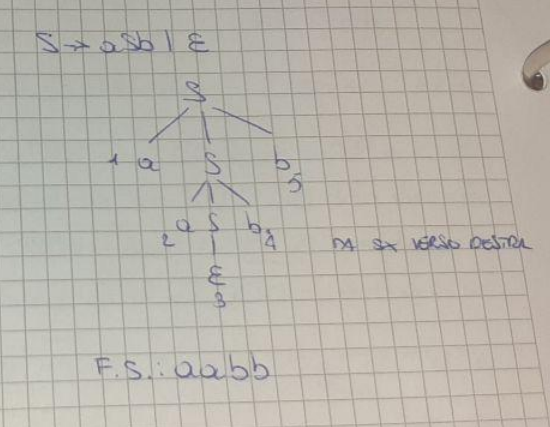
\includegraphics[width=0.75\textwidth]{1}
\end{center}
La computazione di prolog non è altro che una visita di un albero in modo left
most, a seconda di come si visita l'albero infatti cambia ma il prodotto finale
rimane quello.
\\ \\
Dato un albero quindi non c'è un'unica derivazione.
\paragraph{Che rapporto c'è perciò tra alberi e derivazioni?}  
Data una CFG (Grammatica context free) G i seguenti enunciati si equivalgono:
\begin{enumerate}
	\item L'inferenza ricorsiva (quella della tabella in cui in base alla riga
	sapevam dire che valori poteva assumere partendo da quelli precedenti) 
	stabilisce che W (stringa) è nel linguaggio della variabile A
	\item Da A si può derivare in zero o più passi la stringa W
	\item Se esiste una derivazione sinistra di W in 0 o più passi, allora
	esisterà per forza anche una derivazione da destra per W
	\item Esisterà un albero sintattico con radice A e prodotto W
\end{enumerate}
Per esempio: 
\paragraph{fig 5.7 p 175}
\begin{center}
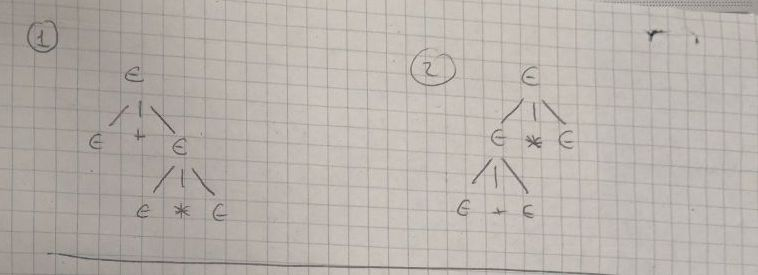
\includegraphics[width=0.75\textwidth]{derivazioneAlbero}
\end{center}
{\color{black} \rule{\linewidth}{0.3mm} }
\\
Nel caso dell'inferenza ricorsiva, si dimostra per induzione ($1 \to 5$) il numero
di passi (righe) dalla inferenza ricorsiva: 
$\begin{cases}
base: ~ A \to w \in P \\
passo~induttivo: ~ Inferenza ~ ricorsiva ~  di ~  n+1  ~ righe, ~  ultima \\ 
~ riga ~  A ~ \underbrace{\to w_{1}, w_{2}, ..., w_{\kappa}}_{w} \leq n ~righe
\end{cases}$
\\
{\color{black} \rule{\linewidth}{0.3mm} }
\begin{center}
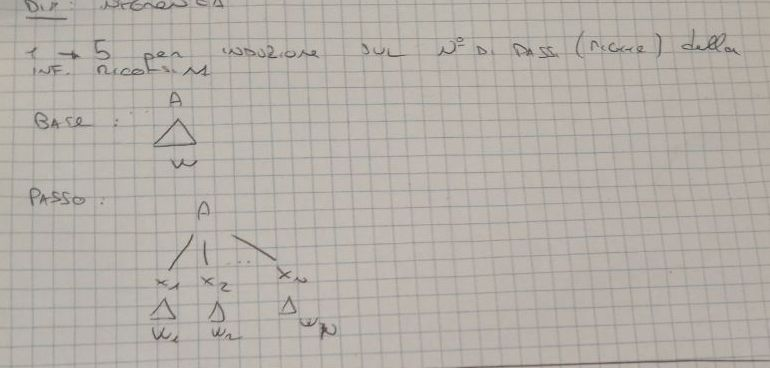
\includegraphics[width=0.75\textwidth]{dimoAlberoInferenza}
\end{center}
{\color{black} \rule{\linewidth}{0.3mm} }
\[E \implies I \implies Ib \implies ab \\
\forall \alpha, \beta \in (V \cup T)^{*} ~vale~ che \\
\alpha E \beta \implies \alpha I \beta \implies \alpha I b \beta \implies
\alpha a ~ b \beta\]
Per induzione sull'altezza dell'albero: 
\begin{center}
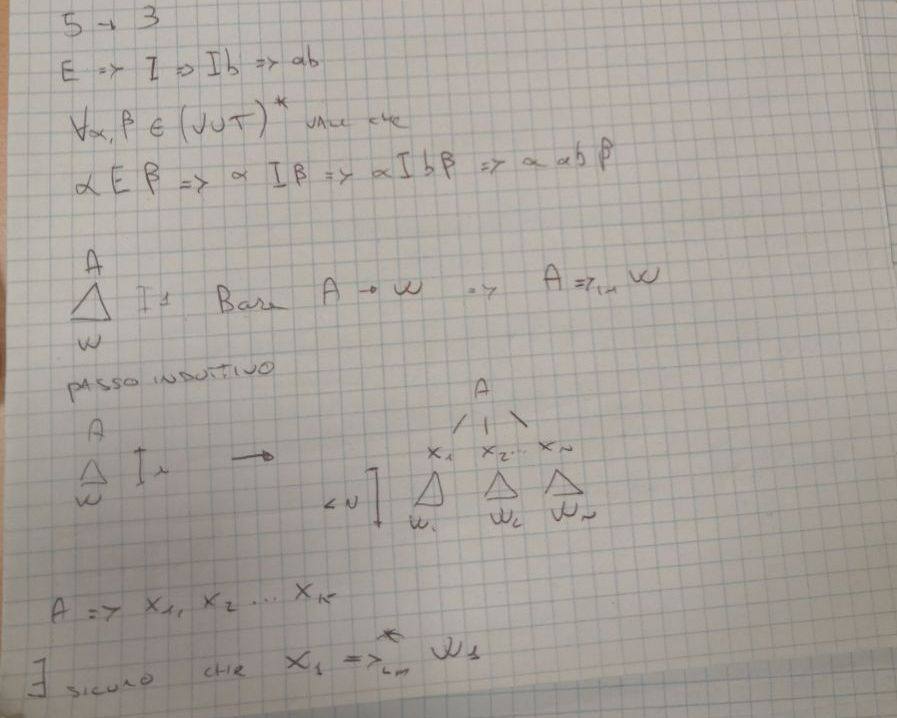
\includegraphics[width=0.75\textwidth]{dimoAltezzaAlbero}
\end{center}
\section{Ambiguità}
E + E * E \\
$E \to E + E | E * E$
1) $E \implies E + E \implies E + E * E$ \\
2) $E \implies E * E \implies E + E * E$
\\
{\color{black} \rule{\linewidth}{0.3mm} }
\begin{center}
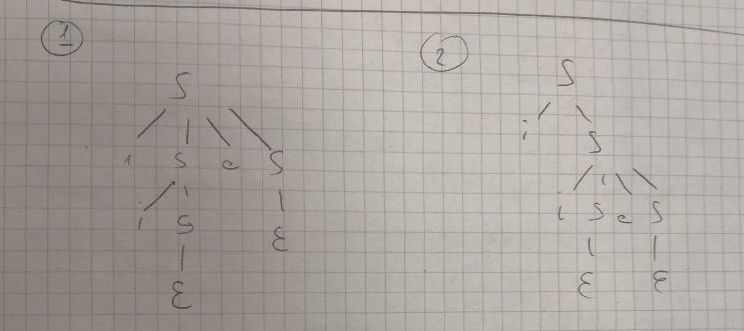
\includegraphics[width=0.75\textwidth]{iSeS}
\end{center}
{\color{black} \rule{\linewidth}{0.3mm} }
\\
\paragraph{Data la seguente CFG: } $S \to \epsilon|SS|iS|iSeS$ \\
Dobbiamo ottenere iie: \\
1) $S \implies iSeS \implies iiSeS \implies iieS \implies iie$ \\
2) $S \implies iS \implies iiSeS \implies iieS \implies iie$
\begin{center}
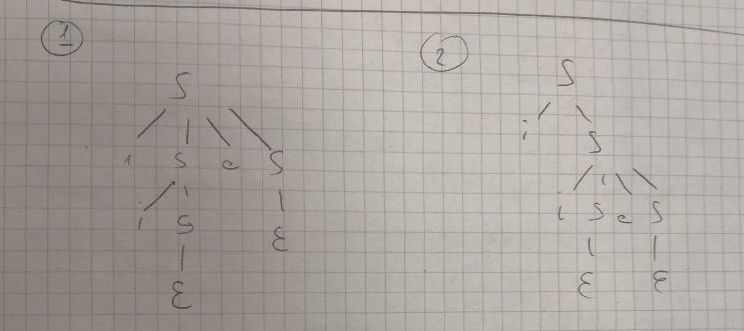
\includegraphics[width=0.75\textwidth]{iSeS}
\end{center}
Se per una stringa ci sono più di un albero sintattico allora essa è ambigua, 
invece non c'è problema se lo stesso albero dia più derivazioni è easy. Ma
perchè è un problema se è ambigua? Perchè non si sa come è cicciata fuori 
fondamentalmente.\\ \\
Non c'è un algoritmo che data una grammatica ti dica se è ambigua o non ambigua,
c'è pure una dimostrazione ma non la vediamo, è uno di quei problemi per cui
non si riesce a trovare una soluzione.\\ \\ Non è detto che una grammatica ambigua
sia trasformabile in una grammatica non ambigua PERO' in realtà in casi tipo 
Linguaggi di Programmazione (la materia dico) o negli XML ci son delle regole
che si sa che funzionino.\\ \\
Ci son linguaggi che sono inerentemente ambigui, ma ora vediamo anche degli esempi.
\paragraph{Riprendiamo gli identificatori: } I $\to$ a|b|Ia|Ib|I0|I1 \\
$F \to I | (E)$ \\
$T \to F | T * F$ \\
$E \to T | E + T$\\
\begin{center}
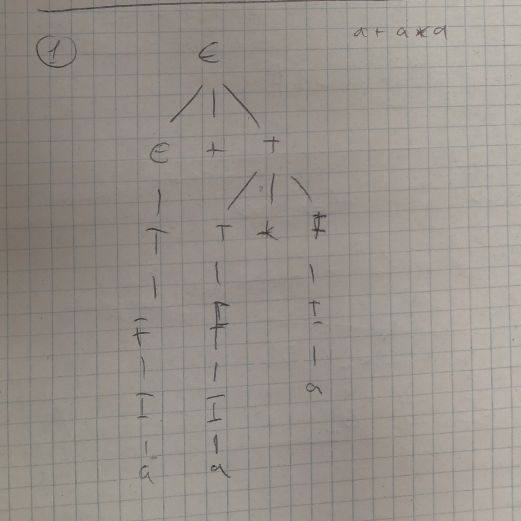
\includegraphics[width=0.75\textwidth]{iSeSB}
\end{center}
\paragraph{Teorema: } $\forall CFG$ \\
G = (V,T,P,S) e $\forall w\in T^{\star}$, w ha due alberi sintattici distinti se e
solo se ha due derivazioni sx distinte. \\
(Solo se): Supponendo due alberi distinti \\
(Se): Supponendo due alberi di derivazioni sx distinte\\ 
C'è un oppure, nel senso che questo è applicabile anche alle derivazioni da dx.
\paragraph{Si ma come fa un albero ad avere due derivazioni sx diverse?}
Esempio:\\
1) $E \to E + E \implies I + E \implies a + E \implies a + E * E \implies A + I * E
\implies a + a * E \implies a + a * I \implies a + a * a $\\
2) $E \implies E * E \implies E + E * E \implies I + E * e \implies a + E * E \implies A + I * E
\implies a + a * E \implies a + a * I \implies a + a * a $ \\ \\ 
Vediamo ora un esempio di linguaggio inerentemente ambiguo: \\
$\nexists$ CFG non ambigua, cioè: \\
L = $\{a^{n} b^{n} c^{m} d^{m} | n, m \geq 1\} \cup 
\{a^{n} b^{n} c^{m} d^{m} | n, m \geq 1\}$ \\
Definiamo le regole di inferenza: \\
\[\begin{cases}
S \to AB|C \\
A \to aAb|ab \\
B \to cBd|cd \\
C \to aCd|aDd \\
D \to bDc|bc 
\end{cases}\]
Ora vediamo come derivare la seguente stringa: "aabbccdd": (n = m - 2) TUTTO LEFT-MOST\\
1) $S \implies AB \implies aAbB \implies aabbB \implies aabbcBd \implies aabbccdd$ \\
2) $S \implies C \implies aCd \implies aaDdd \implies aabDcdd \implies aabbccdd$ \\
\\
Tutti i nodi vanno trasformati in questo, non si può trovare una grammatica 
fondamentalmente. Per non essere inerentemente ambiguo dovrebbe esserci una 
intersezione tra le due, e invece abbiamo ben due derivazioni sinistre diverse.
\\ \\
Per dimostrare davvero che sia inerentemente ambigue bisognerebbe fare una 
dimostrazione vera e propria ma diventa davvero complesso
\section{Grammatiche regolari}
Generano linguaggi di tipo 3 che si chiamano (Regolari) \\
G = (V, T, P, S): Analizziamo le Produzioni (P)\\ \\
Le produzioni hanno i seguenti vincoli:
\begin{enumerate}
	\item $\epsilon$ può comparire solo in $S \to \epsilon$ (S sta per start eh)
	\item Le produzioni sono tutte lineari a dx oppure tutte lineari a sx
	\item \begin{enumerate}
	\item lin a dx: $A \to aB$, oppure A$\to$a con A,B$\in$V e a$\in$T
	\item lin a sx: $A \to Ba$, oppure A$\to$a con A,B$\in$V e a$\in$T
\end{enumerate}
\end{enumerate}
Vediamo subito un esempio:\\
$I \to a|b|Ia|Ib|I0|I1$ lin sx\\
Si vuole rappresentare "b01" da destra verso sinistra\\
$I \implies I1 \implies I01 \implies b01$ \\
In pochi passaggi si è ottenuta subito la nostra stringa \\
Ora invece vediamo il lin dx\\
Ovvero si vuole rappresentare "b01" \\
$I \to a|b|aI|bI|0I|1I$ \\
$I \implies bI \implies b01 \implies b01I ... $ ? \\
Come vediamo non si risolve in questo caso, non esce la stringa, vediamo come fare.
\\ \\
Imponiamoci la regola che:
\[\begin{cases}
I \to aJ|bJ|a|b \\
J \to a|b|aJ|bJ|0J|1J|0|1
\end{cases}\]
Vediamo subito un esempio per capirci meglio: \\
G = (\{S\},\{0,1\},P,S) \\
lin dx: $S \to \epsilon|0|1|0S|1S$ \\
Da qui vediamo che dobbiamo escludere 0 ed 1 poichè
$L(G) = \{0,1\}^{\star}$\\ \\
Ora proviamo a produrre con lin sx 01101: \\
lin sx: $S \implies \epsilon | S0 | S1$
\paragraph{Esercizio} Si forniscano due grammatiche regolari lin dx ed sx per $L
= \{a^{n}b^{n}| n,m \geq 0\}$ \\
\begin{enumerate}
	\item lin dx: G=(\{S,B\}, \{a,b\},P,S)\\
	$S \to \epsilon | aS | bB$\\
	$B \to bB | b$, però così c'è un problema, nel senso che arriva alla B in cui
	può produrre soltando per l'appunto delle b, o comunque arriva che esce con b.
	\\  \\
	Come si risolve questo problema? Aggiungendo la b singola alla prima espressione 
	con S: $S \to \epsilon | aS | bB | \color{red} b \color{black}$
	\item lin sx: G=(\{S,B\}, \{a,b\},P,S)\\
	$S \to \epsilon | Sb | A0| a$ \\
	Con $A \to Aa | a$
\end{enumerate}
\paragraph{Esercizio: } Grammatica lin dx e sx per: \\
L = $\{ab^{n}cd^{m}e | n \geq 0, m \> 0 \}$ \\
\begin{enumerate}
	\item lin dx: \\
	$\begin{cases}
	S \to aA \\
	A \to bA|cB \\
	B \to dB | dE \\
	E \to e 
	\end{cases}$
	\item lin sx: \\
	$\begin{cases}
	S \to Xe\\
	X \to Xd | Yd\\
	Y \to Zc \\
	Z \to Zb | a 
	\end{cases}$
	\item lin dx: (modo equivalente)
	$A \to aB$\\
	$A \to w$\\
	$w\in T^{+}$ \\
	Per esempio: \\
	$A \to ciao \to \begin{cases}
	A \to cB \\
	B \to iC \\
	C \to aD \\
	D \to o
	\end{cases} $
	\item lin sx: \\
	$\begin{cases}
	A \to Bo \\
	B \to Ca \\
	C \to Di \\
	D \to c
	\end{cases}$
\end{enumerate}
\paragraph{Esercizio: } Data G = (\{S,T\},\{0,1\},P,S)\\
$\begin{cases}
S \to \epsilon | 0S | 1T\\
T \to 0T | 1S \\
\end{cases}$
L(G) =$\{w \in {0,1}^{\star} | ~ w ~ contiene~  un~  n ~ pari~  di~  1\}$
\paragraph{Altro esercizio: } Grammatica lin dx ed sx per:\\
L = -$\{w\in \{0,1\}^{\star}-$ | contiene almeno uno 0 oppure almeno un 1\}\\
L = $\{0,1\}^{+}$
\begin{enumerate}
	\item lin dx: G(\{S\},\{0,1\},P,S)\\
	$\begin{cases}
	S \to 0|1|0S|1S
	\end{cases}$
	\item lin sx: G(\{S\},\{0,1\},P,S)\\
	$\begin{cases}
	S \to 0|1|S0|S1
	\end{cases}$
\end{enumerate}
\chapter{Espressioni Regolari}
Esistono linguaggi regolari (Di tipo 3) che possono generare grammatiche regolari(
lin dx oppure lin sx) e rappresentare (\underline{dimostrare}) espressioni 
regolari.\\
Tramite espressioni regolari puoi dimostrare che una stringa fa parte di un 
linguaggio.\\
Inoltre puoi riconoscerle (\underline{accettare}) automi a stati finiti (DFA, 
NFA, $\epsilon$-NFA)
\section{Operazioni sui linguaggi}
\begin{enumerate}
	\item Unione: $L \cup M$ (Unione tra sistemi)\\
	Esempio:\\
	L = \{001,10,111\}
	M =$ \{\epsilon,001\}$
	$L \cup M$ = \{$\epsilon$, 10, 001, 111\}
	\item Concatenazione ($L\cdot M$)\\
	Esempio: \\
	L = \{001,10,111\}
	M = $\{\epsilon,001\}$
	$L \cdot M$ = \{$\epsilon$001, $\epsilon$10, $\epsilon$111, 001001, 10001, 111001\}	 
	\item Chiusura di Kleene: $L^{\star}$ \\
	L =$ \bigcup \limits _{i=1} L^{1} = \bigcup \limits _{i=1}^{\infty} L^{1}$\\
	Dove: $L^{0} = \{\epsilon\}, L^{1} = L$, fino ad arrivare a $L^{i}$ =
	$\underbrace{LLLLL...L}_{i~volte} $	i volte (per i $\geq$ 1)\\
	Esempio: \\
	L = \{0,11\} \\
	$L^{\star} = \{\epsilon\} \cup \{0,11\} \cup \{00,011,110,1111\} \cup 
	\{000,0011,01111,1100,11011,11110,111111\} \cup$ ...
\end{enumerate}
Ci sono dei casi particolari 
\begin{enumerate}
	\item $L = \varnothing $ (Non contiene stringhe)
	\item $L = \{\epsilon\} $(Cotiene solo la stringa vuota)
	\item $\varnothing = {\epsilon}$
	\item$ \varnothing^{i} = \varnothing ~~~ \forall i\geq1$
	\item $\varnothing^{\star} = \varnothing^{0}, \varnothing^{1}, ..., 
	\varnothing^{n}$
	\item $\{\epsilon\}^{\star} = \{\epsilon\}^{1}, \{\epsilon\}^{2}, ...,
	\{\epsilon\}^{n}$  = $\{\epsilon\}$
	\item Qualunque insieme se non vuoto, e non avente solo la stringa vuota,
	è in grado di generare qualsiasi stringa, di lunghezza che può estendersi
	fino ad $\infty$
\end{enumerate}
Tornando alle epsressioni regolari: \\
Si dice che esse denotino linguaggi regolari, dice come sono fatte le stringhe, 
in maniera più esplicita e compatta di una grammatica, e si definiscono 
in modo ricorsivo,(matematicamente per induzione, sempre lì si torna).\\ \\
Ci saranno dei casi base e una serie di passi, vediamo i 3 casi base:
\begin{enumerate}
	\item $\epsilon, \varnothing$ sono espressioni regolari, perciò $\epsilon$ ha 
	già più di un significato, di solito si indica in grassetto, per comodità
	in questo contesto sappiamo che indica un'espressione regolare (\textbf{$\epsilon$})\\
	L($\epsilon)$ = $\{\epsilon\}, L(\varnothing) = \varnothing$
	\item Se a $\in \Sigma$, a è una espressione regolare \\
	L(a) = \{a\}
	\item Variabili che rappresentano linguaggi: (L per esempio) sono espressioni
	regolari
\end{enumerate}
Vediamo ora i seguenti passi induttivi:
\begin{enumerate}
	\item Unione: Se E, F sono ER, allora E+F è una ER (E+F = L(E) $\cup$ L(F))
	\item Concatenazione: Se E, F sono ER, allora EF è una ER (L(EF) = L(E)L(F))
	\\ Ad esempio \\
	$\Sigma^{1} = \{0,1\}$, E = 0, F = 1 EF=01
	\item Chiusura: Se E è una ER, allora $E^{\star}$ è una ER $(E^{\star}=(L(E))^{\star})$
	\item Parentesi: Se E è una ER, allora (E) è una ER (  L((E))=L(E)  ) \\
	Vedrete lisp, a proposito di parentesi..
\end{enumerate}
\section{Precedenza operatori}
\begin{enumerate}
	\item Chiusura di Kleene ($\star$)
	\item Concatenazione A $\circ$ B
	\item Associativa, commutativa (l'unione) 
\end{enumerate}
\section{Esercizi}
\paragraph{Es. 1}
Data la seguente ER = $(0+1)^{\star} 0^{\star} (01)^{\star}$ \\
Dire se 001 è reaizzabile con il suddetto insieme: \\
$(0+1)^{\star}$ = 1 0 1 0\\
$L((0+1)^{\star}) = (L(0+1))^{\star} = (L(0)\cup L(1))^{\star} = (\{0\} \cup \{1\})
= (\{0,1\})^{*}$, quindi è possibile realizzarlo
\paragraph{Es. 2}
Data la seguente ER = $0^{\star} (01)^{\star}$ \\
Dire se 001 è reaizzabile con il suddetto insieme: \\
001 Si'
1001 NO \\
0101 Si' \\
\section{Identità ed annichilatori}
\subsection{L'identità} E' un valore tale per cui la somma con esso (identità +
valore) darà il valore stesso (a+x = x+a $\forall x \in$ ESISTENZA)\\
$\varnothing$ è un'identità per +: $\varnothing + E = E + \varnothing = E$ \\
$\epsilon$ è identità per$ \circ: \epsilon E = E\epsilon = E$ \\
\subsection{Annichilatore}
$\varnothing $è annichilatore per$ \circ: \varnothing E = E \varnothing = \varnothing$
\paragraph{Esercizio tipo esame}
Data ER = $((01)^{\star}10(0+1)^{\star})^{\star}$
E' possibile realizzare 0101? Nope\\
01000? Nemmeno \\
01011 Nemmeno \\
10111 SI PUO' FARE WOOOOO (Perdonatemi, lo svolgimento lo aggiungerò successivamente
quando ci studierò sopra, perchè al momento mi è troppo lungo scriverlo)
\section{Distributività}
Aritmeticamente se ho $x(y+z)$, posso riscriverlo come $xy+xz$.
Consideriamo due tipi di distributività:
\begin{itemize}
	\item Distributività SX della concatenazione rispetto all'unione: \\
	$L(M+N) = LM + LN$
	\item Distributività DX: $(M+N)L = ML + NL$
\end{itemize}
\paragraph{Vediamo subito un esempio: } Data una ER `$0+01^{\star}$`
\[
L(0+01^{\star}) = L(0) + L(01^{\star}) = \{0\} \cup L(0)L(1^{\star}) =
\]
\[
= \{0\} \cup \{0\} (L(1))^{\star}) = \{0\} \cup \{0\} \{1\}^{\star} = 
\]
\[
\{0,01,011,0111, 01111, ...\}
\]
Con:
\[
\begin{cases}
\{1\}^{\star} = \epsilon, 1, 11, 111, 1111, ... \\
\{0\} \{1\}^{\star} = \epsilon, 01, 011, 0111, 01111, ...
\end{cases}
\]
A questo punto passiamo a considerare `$0+01^{\star}$`:
\[
0+01^{\star} = 0\epsilon + 01^{\star} = 0(\epsilon + 1^{\star}) = 01^{\star}
\]
\[
= (0(\epsilon + 1^{*})) = L(0) L(\epsilon + 1^{*}) = 
\]
\[
= \{0\} (\{\epsilon\} \cup L(1))^{*}) ...
\]
\section{Idempotenza}
Dal punto di vista dell'unione si ha che L + L = L, ma se visto aritmeticamente
viene leggermente più chiaro da capire, infatti:
\[x+x\neq x\]
La somma non gode dell'indepotenza
\[x\cdot x\neq x\]
Ed allo stesso modo non ne gode nemmeno il prodotto
\section{Proprietà chiusura}
\[
(L^{\star})^{\star} = L^{\star}
\]
\[
(L^{\star})^{\star} = \bigcup \limits _{i \geq 0} {(L^{\star})^{i}}
\]
Da questo si deriva che $\varnothing^{\star}=\epsilon$ e $\epsilon^{\star}=\epsilon$,
ora passiamo ad $L^{+}$
\[
L^{+} = LL^{*} = L^{*}L = L + LL + LLL + LLL = L\epsilon + LL * LLL =
\]	
\[
L(\epsilon + L + LL + LLL * ....) = LL^{*}
\]	
\paragraph{Esercizio 1: } Data ER = $(00^{*}1^{*})^{*}$\\ 
Fin da subito osserviamo che avremo una serie di blocchi tutti inizianti per
0 di questo tipo: $0xxxx0xxxx0xxxx$, potrebbero capitare blocchi aventi una
serie di 0 ed una serie di 1. 
\begin{itemize}
	\item Posso avere una stringa tutta di 1? No
	\item Una stringa avente uno 0 e tutti 1? Sì
\end{itemize}
Non l'ho specificato ma $\epsilon \in L$ \\
Quello che si nota è che quindi ogni stringa che avrò inizia per 0, perciò potrò
scrivere qualcosa del tipo $0(0+1)^{*} + \epsilon$
\paragraph{Esercizio 2: } Quale linguaggio si denota da questa ER: $a(a+b)^{*}b$?\\
L = $\{w \in \{a,b\}^{*} |$ w inizia con a e termina con b\}, spiegato peggio 
sarebbero tutte le strinche che iniziano con a e b, ed all'interno hanno 
qualsiasi combinazione
\paragraph{Esercizio 3: } Quale linguaggio si denota da questa ER: $(0^{*}1^{*})000(0+1)^{*}$?\\
E' in pratica come dire, qualsiasi insieme di 0 ed 1 (zeri ed uni) che in mezzo
da qualche parte avranno un punto in cui ci sarà una sequenza di 3 zeri
\paragraph{Esercizio 4: } Quale linguaggio si denota da questa ER: $a(a+b)^{*}c(a+b)^{*}c(a+b)^{*}b$?\\
L = \{$w\in \{a,b,c\}$ | w inizia con a, termina con b, e contiene esattamente DUE c\}
\paragraph{Esercizio 5: } Scrivere un'ER per questo linguaggio: 
L = $\{w\in \{0,1\}\}$ | in w, tutte le coppie 11 seguono tutte le coppie 00, 
nel senso:
\[
L = L_{11}L_{00} 
\]
Attenzione, tutte le coppie 11 SEGUONO tutte le coppie 00, quindi da un lato
si hanno tutti gli 00 e dall'altra 11: 0011, 00001111, 0000000011111111 
\subparagraph{Proviamo a scrivere le ER } 
\begin{itemize}
	\item Per $L_{11}$: $(10+0)^{*}(\epsilon + 1)$
	\item Per $L_{00}$: $(01+0)^{*}(\epsilon + 0)$
\end{itemize}
Ed infine proviamo a scrivere l'ER per L:
\[
(10+0)^{*} (\epsilon + 1) (01+1)^{*} (\epsilon + 0)
\]
Si può addirittura elidere $(\epsilon + 1)$ poichè comparirebbe nella parentesi
dopo.
\chapter{Automi a stati finiti deterministici (DFA)}
Sono insiemi di stati legati da una serie di archi di transizione, e sono 
strettamente legati ai linguaggi regolari, perchè sono generati da grammatiche 
regolari, cioè di tipo 3, ed accettati da DFA. \\ \\
O meglio, le stringhe generate dalla grammatica regolare posso darli in pasto
al mio automa in grado di leggere la stringa carattere per carattere, e 
quest'ultimo sarà in grado di dirmi se codesta stringa è generabile. \\ \\
Inoltre sono denotati da espressioni regolari
\section{Come sono fatti}
Ecco un esempio di DFA
\begin{center}
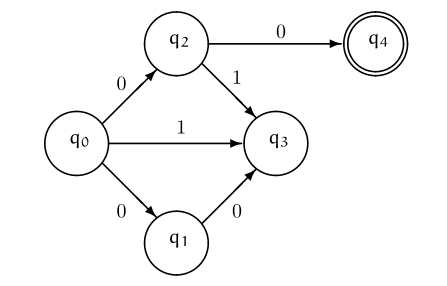
\includegraphics[width=0.75\textwidth]{dfa}
\end{center}
Però bisogna anche adesso includere alcune cose: 
Ogni automa ha una casellina in cui si può inserire un carattere, pertanto avremo
un alfabeto $\Sigma$.\\ \\
Perciò si ha un insieme di stati (\textbf{Q}), un sotto insieme di \textbf{Q} che
son stati finali $F\subseteq Q$ \\
Dato un linguaggio regolare si ha un automa che entra in stato finale SE esaminata
carattere per carattere la stringa si arriva fino alla fine.
\\
{\color{black} \rule{\linewidth}{0.3mm}}
\paragraph{Rappresentazione di Gaia più accurata}
\begin{center}
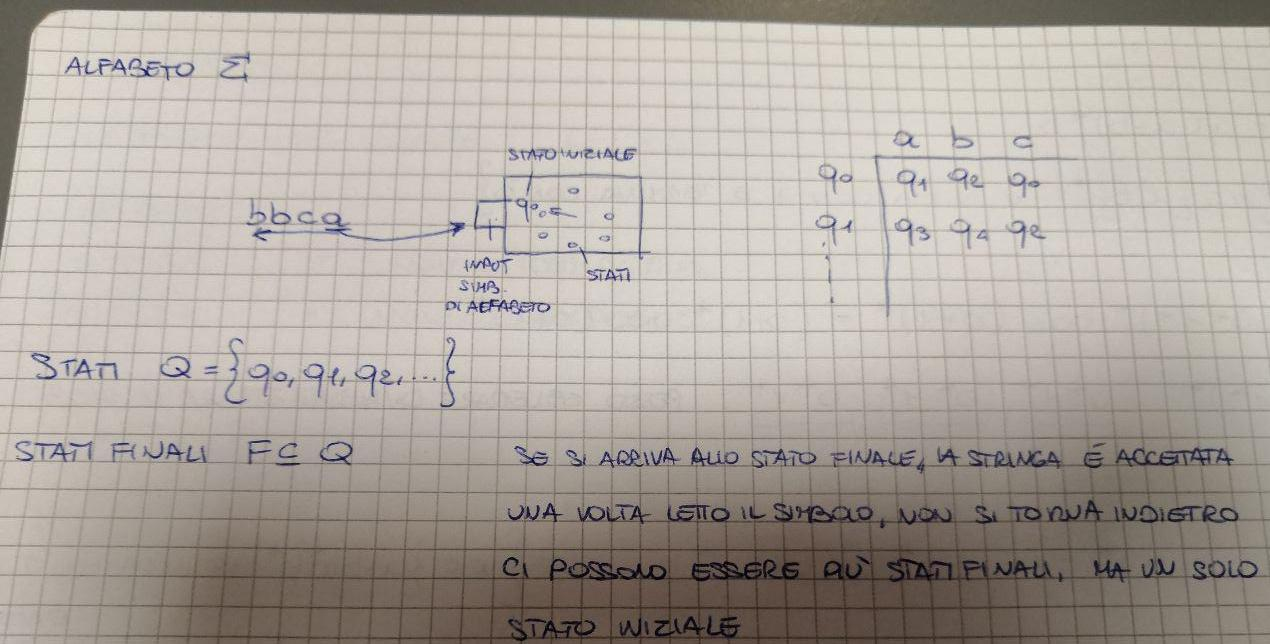
\includegraphics[width=0.75\textwidth]{rappreDFA}
\end{center}
{\color{black} \rule{\linewidth}{0.3mm}}
\\
\paragraph{Osservazione: } Una volta letto un simbolo, viene consumato, essa
sparisce, non viene più ripresa. In aula è stato fatto l'esempio di un mitra, che
spara i colpi uno dopo l'altro ed una volta sparato non c'è modo di recuperare
un colpo.
\section{Definizione formale}
E' una quintupla in cui:
\begin{itemize}
	\item Q è l'insieme finito degli stati
	\item $\Sigma$ è l'alfabeto delle stringhe date in input
	\item $\delta$ è la funzione di transizione degli stati
	\item $q_{0}\in Q$ è lo stato iniziale
	\item $F \subseteq Q$ è l'insieme degli stati finali
\end{itemize}
In pratica $\delta:Qx\Sigma \to Q$ che riassunto vuoldire, prendo uno stato, 
una lettera dell'alfabeto, e rimango nello stato. E $\delta(q,a) = p$
\paragraph{Esercizio 1: } Generare un DFA che accetti w$\in \{0,1\}^{*}$ | w
contiene un numero pari di 1 \\ \\
A = $(\{q_{p}, q_{d}\}, \{0,1\}, \delta, q_{p}, \{q_{p}\}) $(La p sta per pari,
la d per dispari)
\begin{itemize}
	\item $\delta(q_{p}, 0) = q_{p}$
	\item $\delta(q_{d}, 0) = q_{d}$
	\item $\delta(q_{p}, 1) = q_{p}$
	\item $\delta(q_{d}, 1) = q_{d}$
\end{itemize}
A questo punto è necessario fare la nostra tabella 2 x 2 
\begin{center}
\begin{tabular}{ | c | c | c }
/ &  0 & 1 \\ 
$q_{p}$ & $q_{p}$  &  $q_{d}$ \\  
$q_{d}$ &  $q_{d}$ & $q_{p}$     
\end{tabular}
\end{center}
Il disegno dell'automa non l'ho fatto io, ringrazio Gaia (ormai son più suoi
che miei questi magici appunti)
\begin{center}
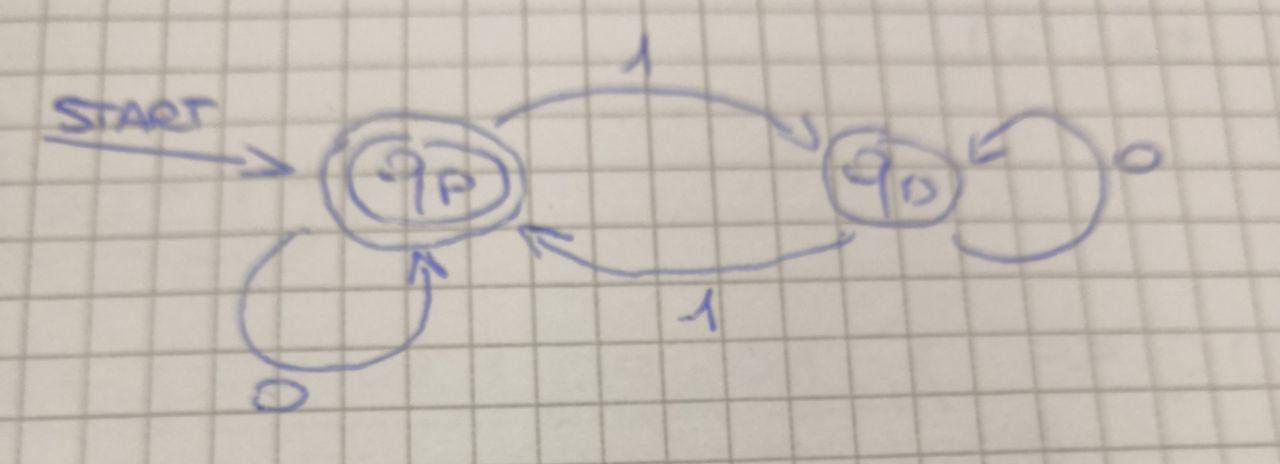
\includegraphics[width=0.75\textwidth]{2}
\end{center}
\paragraph{Esercizio 2: } Definire una ER per L = \{w$\in \{0,1\}^{*}$ | w
contiene un numero pari di 1\} \\ \\
In pratica prima abbiamo generato l'automa, a questo punto proviamo a definire
una ER $\to (0^{*},1,0^{*},1)^{*}0^{*}$
\paragraph{Esercizio 3: } Progettare un DFA che accetti 
L=$\{x01y|x, y\in\{0,1\}^{\star}\}$. Per prima cosa bisogna ragionare su quali
sono le più corte stringhe che il linguaggio accetti, e si verifica che la
stringa più corta sia $01 \in L$\\ \\
Consideriamo che uno stato iniziale si indica con una freccia esterna che si 
chiami start, e lo stato finale invece sia un cerchio dentro l'altro.
Il nostro automa risulterà: A = $(\{q_{0}, q_{1}, q_{2}\},\{0, 1\},\delta,q_{0},\{q_{1}\})$\\
(I successivi automi sono stati fatti da \href{https://github.com/LiaBell47}{Giulia})
\begin{center}
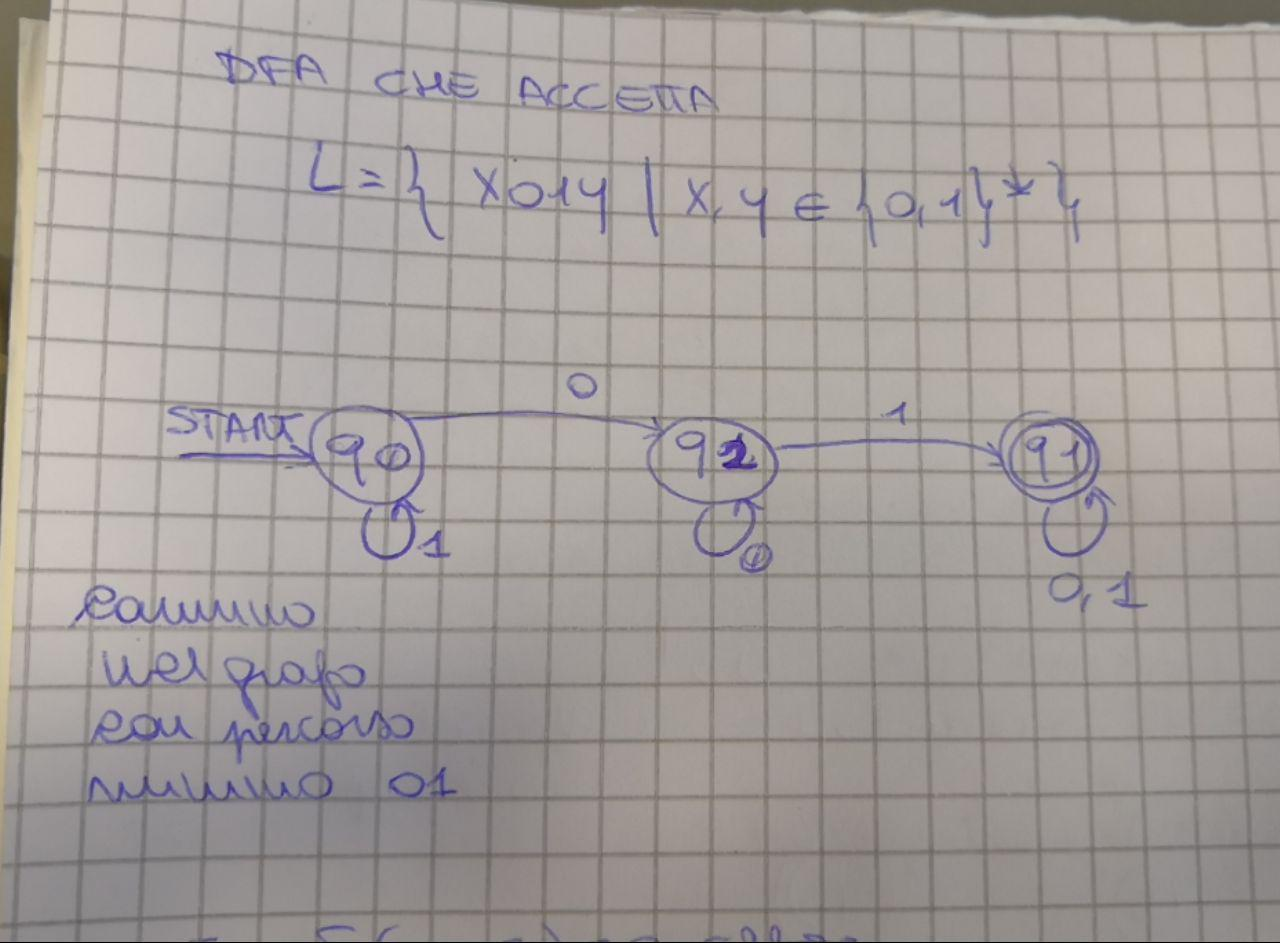
\includegraphics[width=0.75\textwidth]{3}
\end{center}
in cui $\delta(q_{0},0)=q_{2}$
\paragraph{Esercizio 3:} Stabilire ER per L = $\{w \in \{0, 1\}^{\star}\}$ | w
contiene un numero di 0 divisibile per 3\}
\subparagraph{Soluzione: } ER = $(1^{*}01^{*}01^{*}0)^{*}1^{*}$
\paragraph{Osservazione: } Un DFA non è in grado di rappresentare delle CFG, e 
questo perchè un automa a stati finiti ha della memoria finita. Per questa 
ragione, non può appunto rappresentare delle Context Free
\paragraph{Esercizio 4: } Progettare un DFA per L = $\{w\in\{0,1\}^{\star} | w = 0^{n}1^{n}\}$ con:
\begin{itemize}
	\item n,m $\geq$ 0
	\begin{center}
	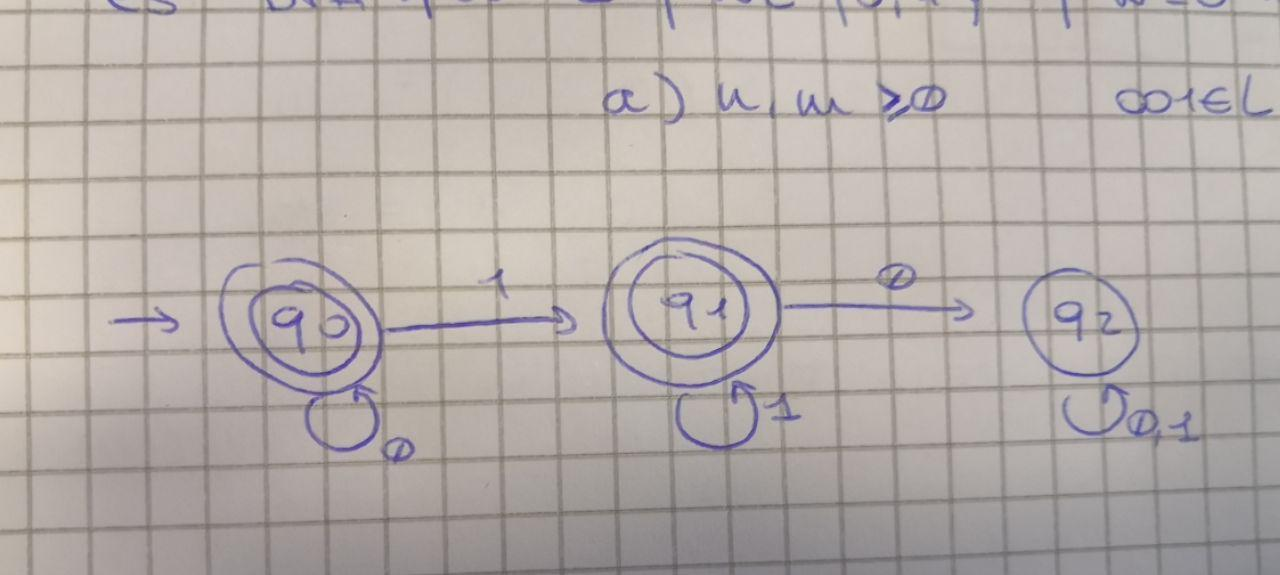
\includegraphics[width=0.75\textwidth]{4}
	\end{center}
	A = $(\{q_{0}, q_{1}, q_{E}\},\{0, 1\},\delta,q_{0},\{q_{1}\})$
	\item n$\geq 0, m>0$
	\begin{center}
	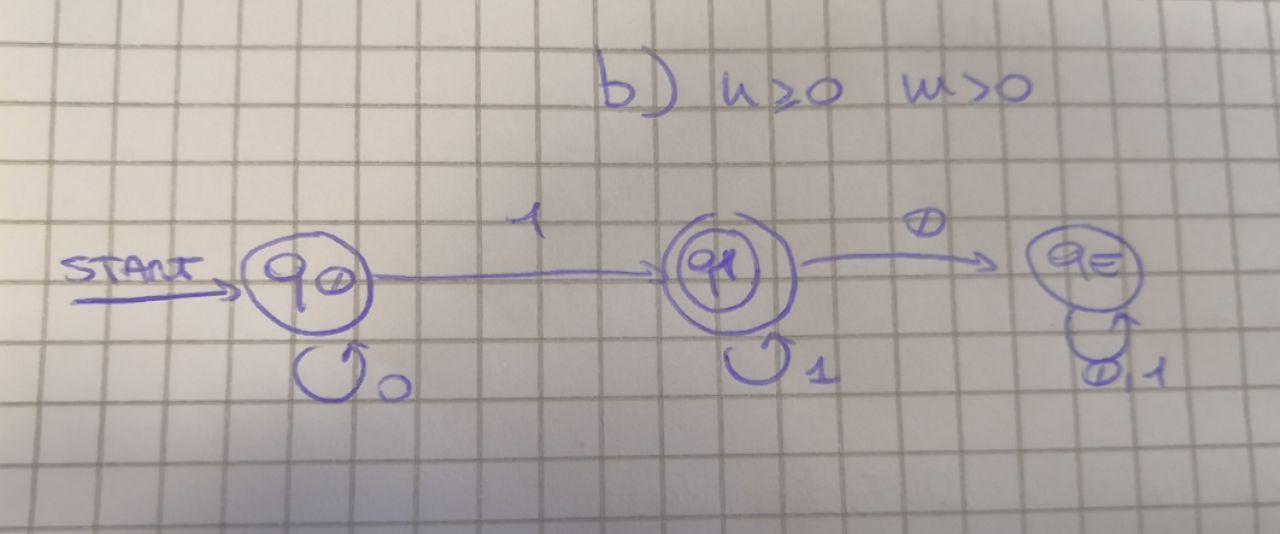
\includegraphics[width=0.75\textwidth]{5}
	\end{center}
	\item n > 0, m$\geq$ 0, $\epsilon \notin L, 0 \in L$
	\begin{center}
	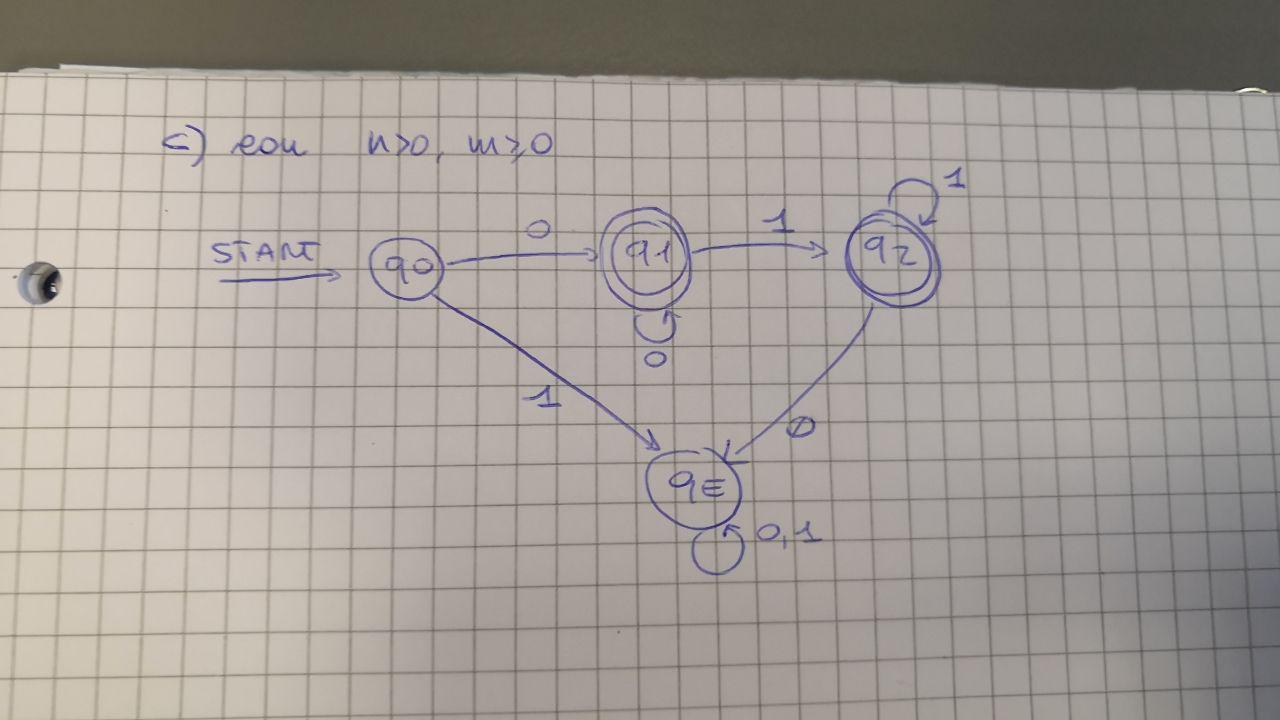
\includegraphics[width=0.75\textwidth]{6}
	\end{center}
	\item n > 0, m > 0
	\begin{center}
	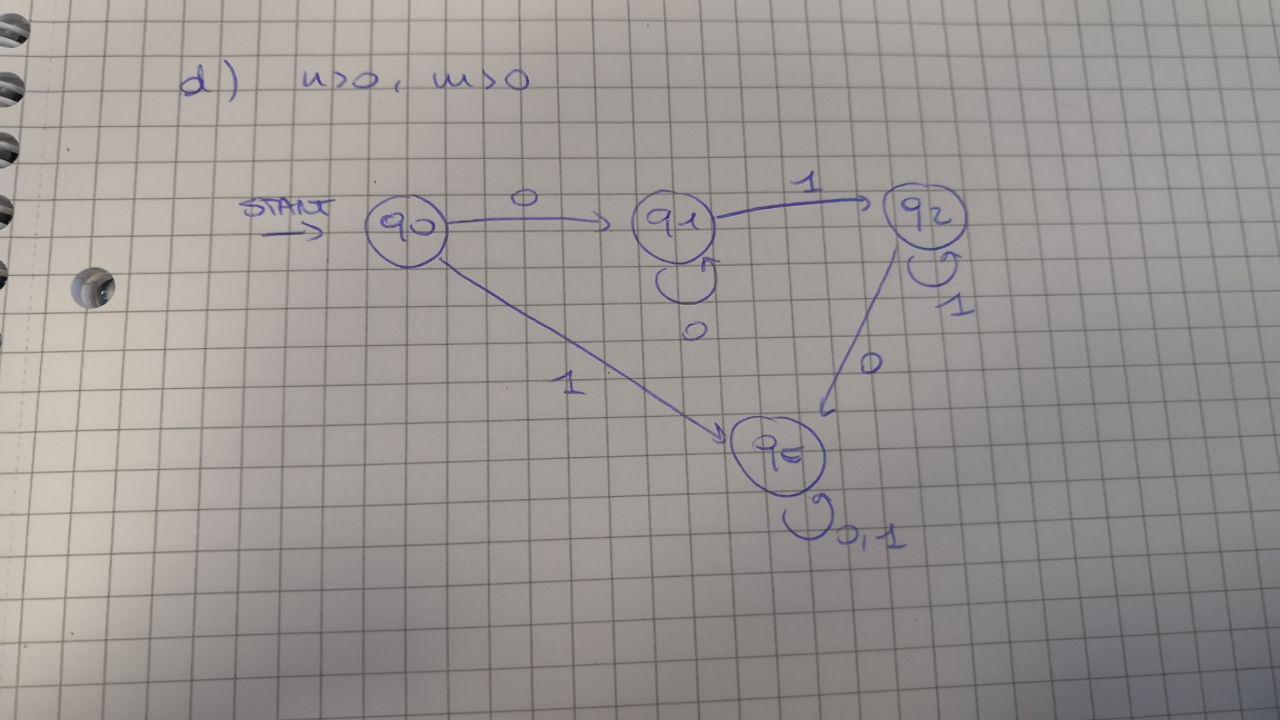
\includegraphics[width=0.75\textwidth]{7}
	\end{center}
\end{itemize}
($q_{E}$ sarebbe lo stato di errore)
\paragraph{Esercizio 5: }Progettare un DFA per L = $\{w\in \{a,b\}^{\star}$|\}
w contiene un numero pari di a ed un numero dispari di b\}
\begin{center}
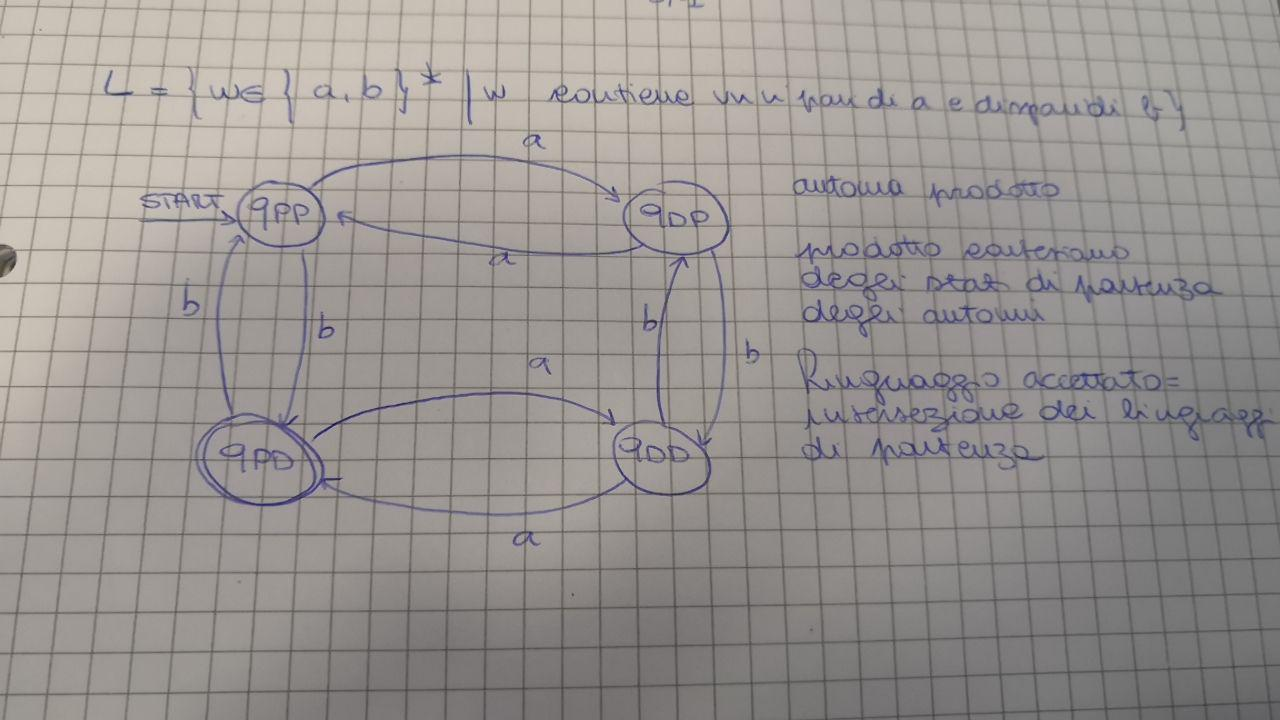
\includegraphics[width=0.75\textwidth]{8}
\end{center}
Come si può osservare è un automa molto regolare, perchè in qualche modo
si prende l'automa che riconosce le a pari, uno che riconosce le b dispari e 
si sono accostati i due tra di loro (Ok, è informale, esiste l'automa prodotto,
Ma lo vedremo in seguito)
\paragraph{Esercizio 6: } Progettare un DFA per L = $\{w\in \{a,b\}^{\star}\}$|
w contiene un numero pari di a \textbf{seguito} da un numero
dispari di b $\implies \{a^{2n}b^{2k+1}\} | n, k \geq 0\}$
\begin{center}
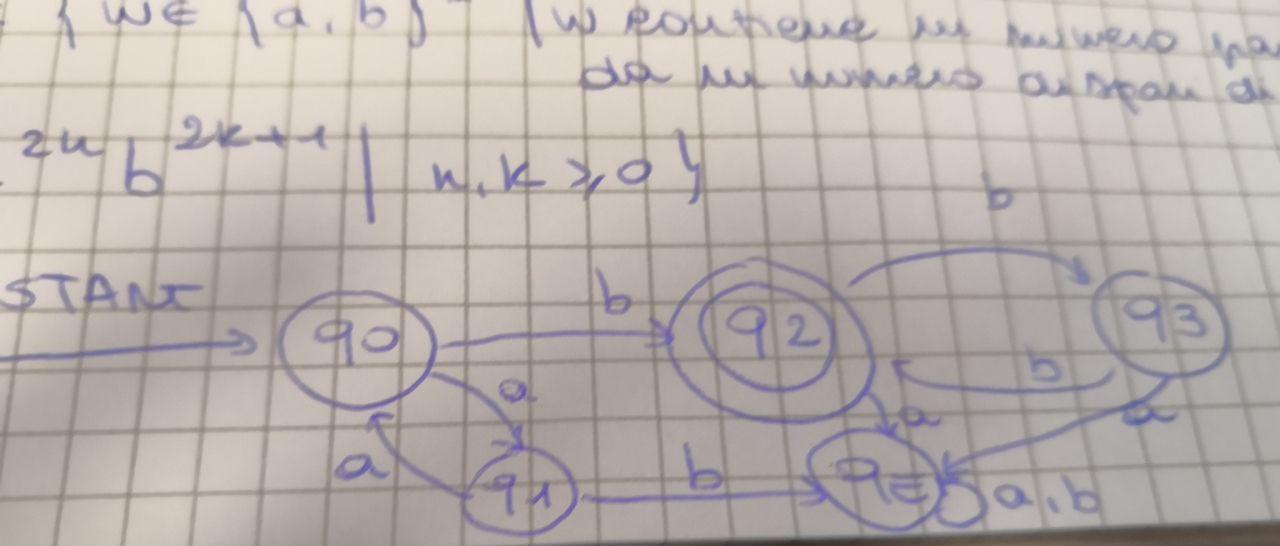
\includegraphics[width=0.75\textwidth]{9}
\end{center}
\section{Estensione di $\delta$}
Finora si è detto che $\delta:Q \times \Sigma \to Q$ e $\delta(q,a) = p$ 
L'estensione $\widehat{\delta}:Q \times \Sigma^{\star}\to Q$ \\ \\
Se $w\in \Sigma^{\star}, \widehat{\delta}(q,w) = p$\\ \\
\paragraph{Torniamo all'esercizio 6} In questo caso quindi, si scriverà:
\begin{center}
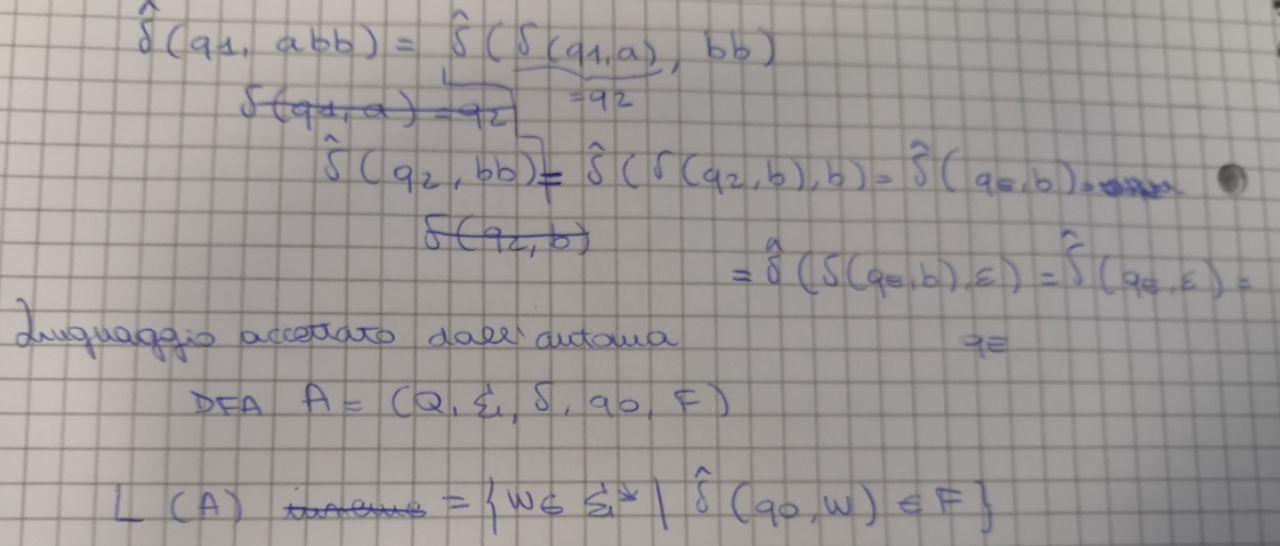
\includegraphics[width=0.75\textwidth]{10}
\end{center}
\paragraph{Esercizio 7: }
\begin{center}
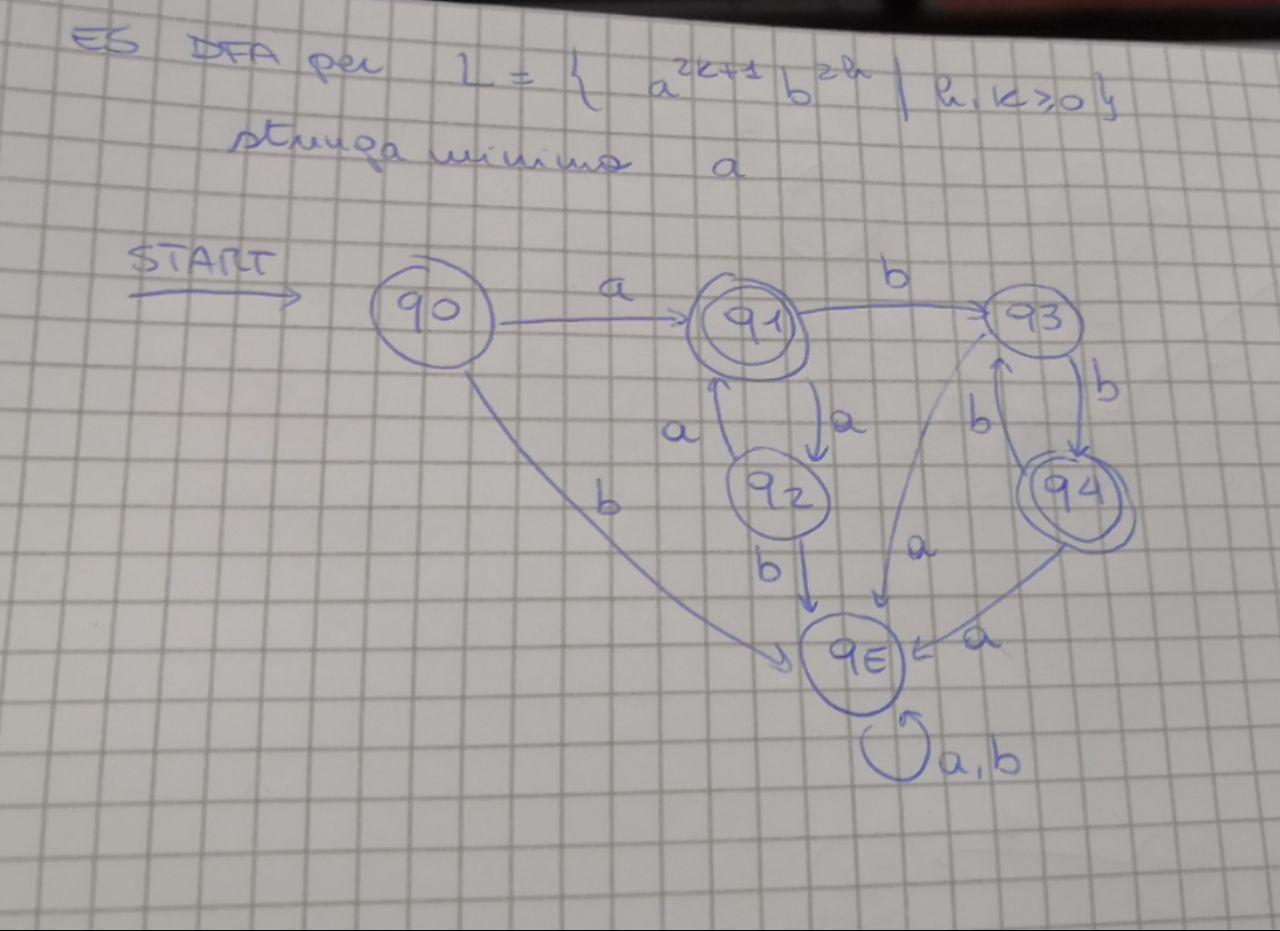
\includegraphics[width=0.75\textwidth]{11}
\end{center}
\paragraph{Esercizio 8: }
\begin{center}
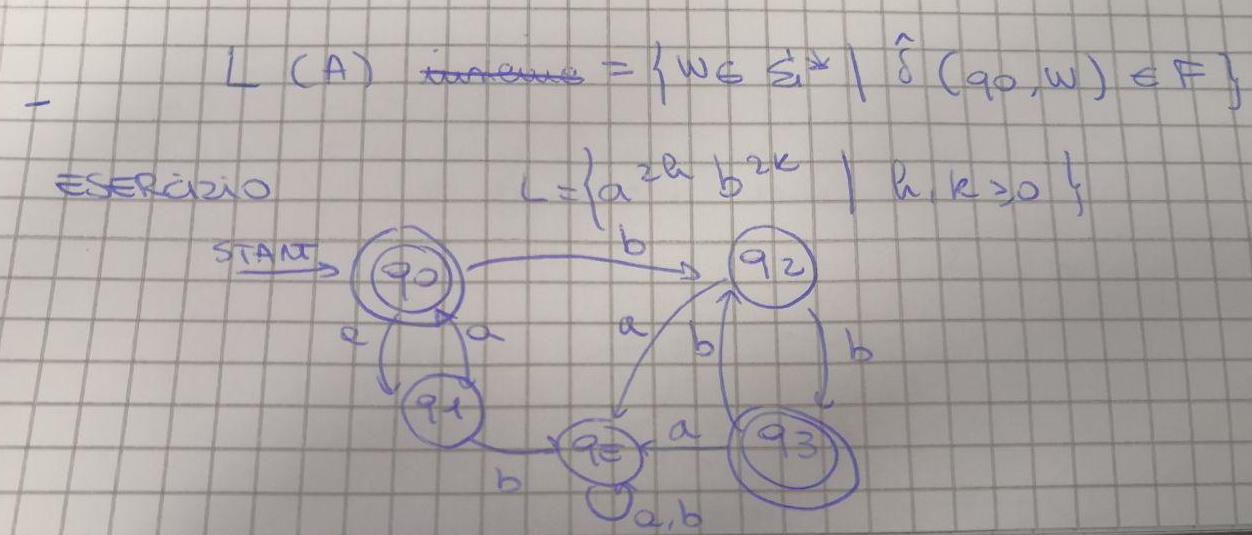
\includegraphics[width=0.75\textwidth]{12}
\end{center}
\paragraph{Esercizio 8: }Produrre una ER per L =$ \{w\in \{0,1\}^{\star} $| 
contiene al più (al massimo) una coppia di 1 consecutivi\}
\[
(10+0)^{*}(11+1+\epsilon)(01+0)^{*}
\]
Il primo blocco non può essere ($1+0^{*}$) perchè altrimenti verrebbero fuori in 
mezzo anche coppie di 11.
\paragraph{Esercizio 9: }
Produrre una ER per L = $\{w \in \{a,b,c\}^{*}$ | w contiene almeno una a e almeno
una b\}
\[
c^{*}(a(a+c)^{*}b+b(b+c)^{*}a)(a+b+c)^{*}
\]
\paragraph{Esercizio 10: }
Progettare un DFA per L = $\{w \in \{0,1\}^{*} | w = x010y, ~con~x,y\in\{0,1\}^{*}\}$ 
\begin{center}
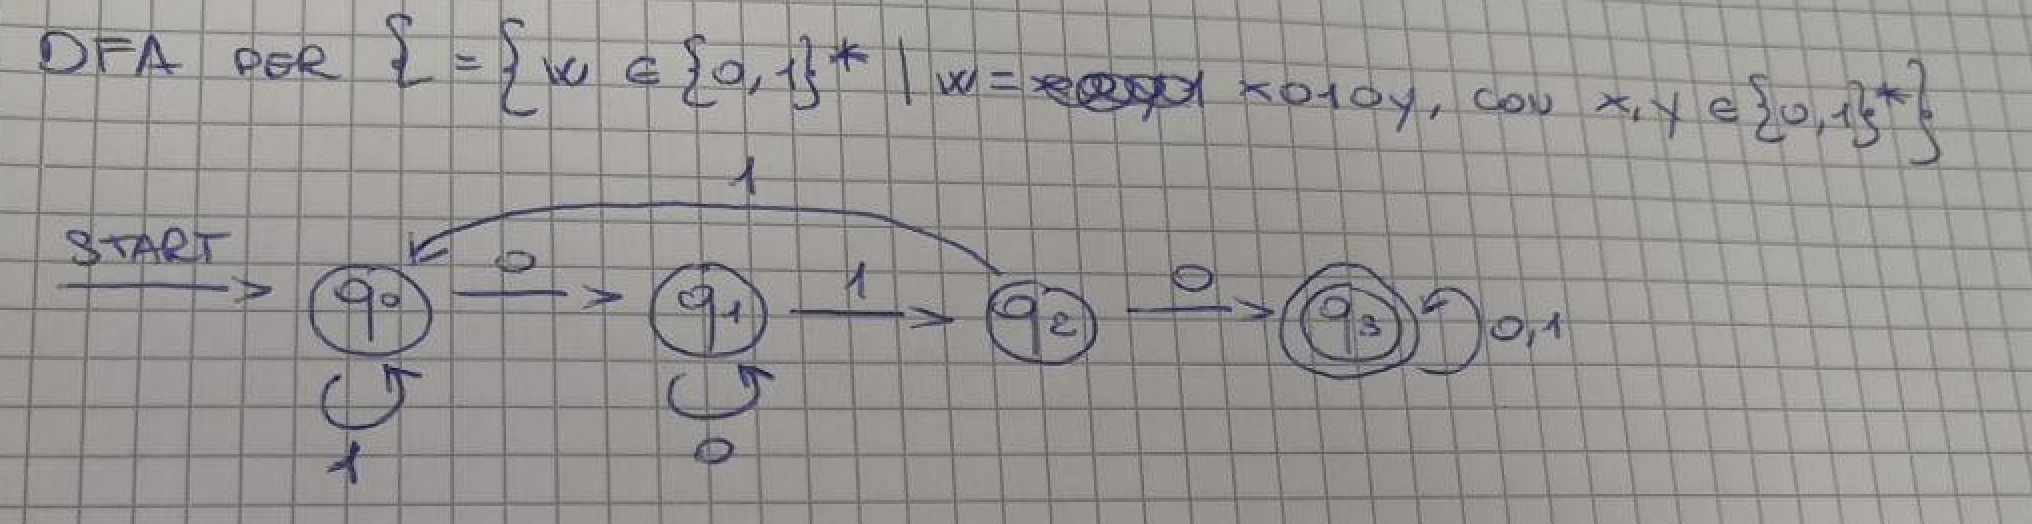
\includegraphics[width=0.75\textwidth]{13}
\end{center}
\paragraph{Esercizio 11:}
Progettare un DFA per L = $\{w \in \{0,1\}^{*}$ | le coppie 00 precedono le 
coppie 11\}
\begin{center}
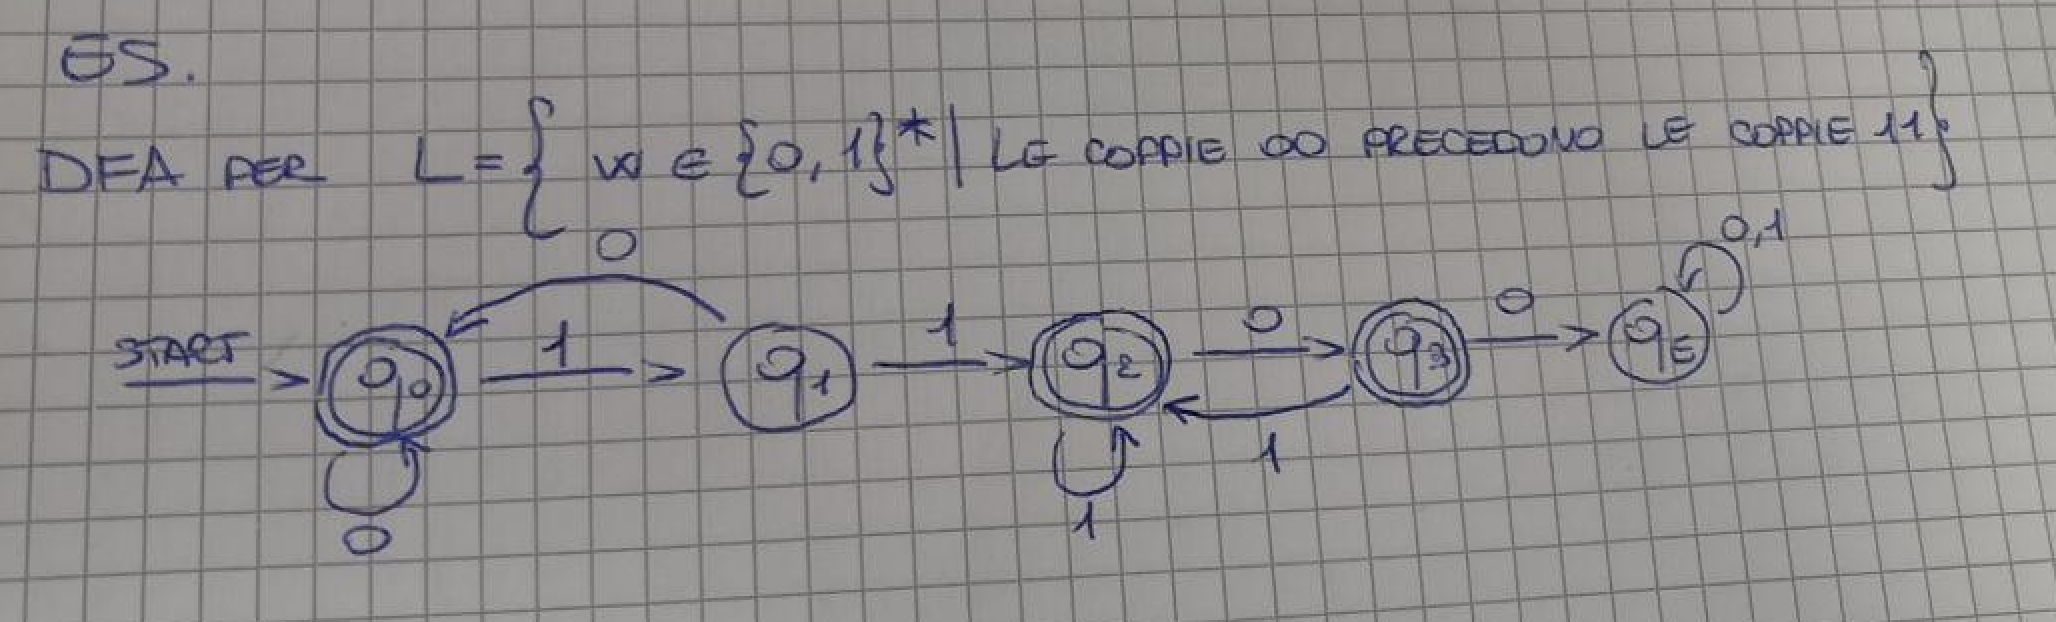
\includegraphics[width=0.75\textwidth]{14}
\end{center}
\paragraph{Esercizio 12:}

Dato il seguente DFA:
\begin{center}
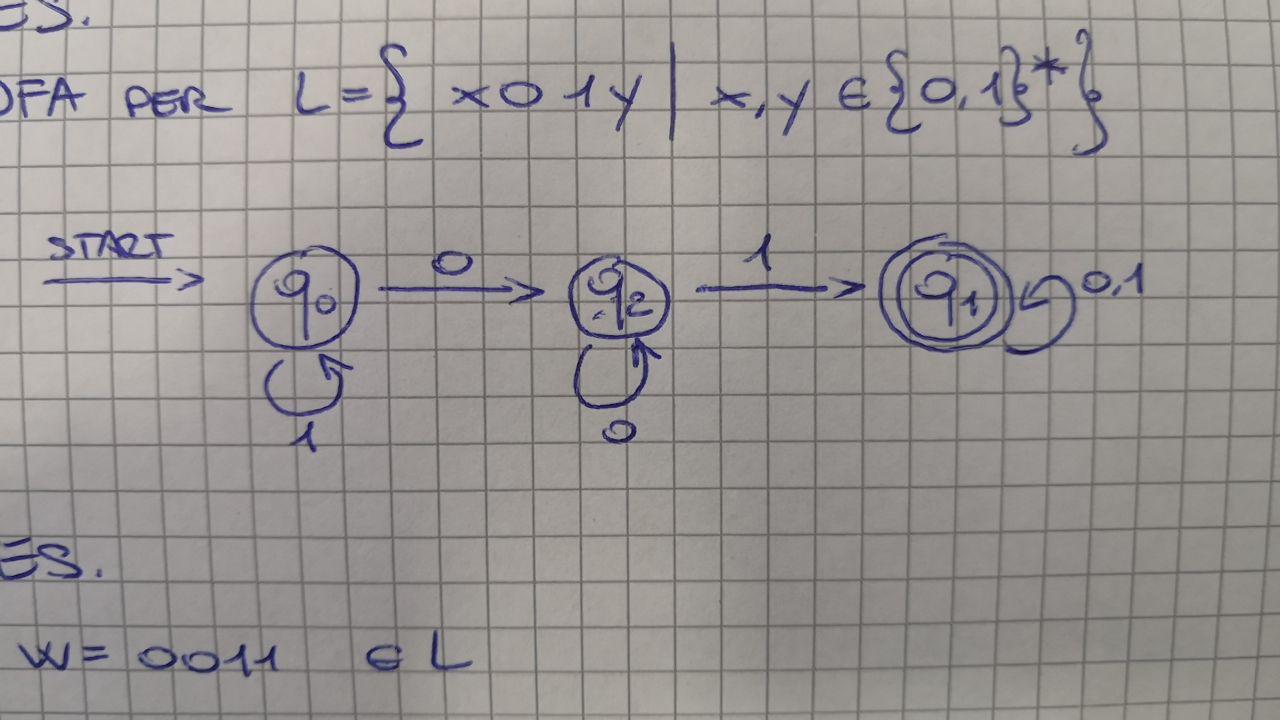
\includegraphics[width=0.75\textwidth]{15}
\end{center}
Consideriamo la stringa w = 0011 $\in$ L
$\widehat{\delta}(q_{0}, 0011$ = $\widehat{\delta}(\delta(q_{0},011))$ =
$\widehat{\delta}(q_{2},011)$ = $\widehat{\delta}(\delta(q_{2},0).11)$ = 
$\widehat{\delta}(q_{2},11)$ = $\widehat{\delta}(\delta(q_{2},q)$ = 
$\widehat{\delta}(q_{1},1)$ = $\widehat{\delta}(\delta(q_{1},1),\epsilon)$ = 
$\widehat{\delta}(q_{1}, \epsilon) = q_{1}\in F \to w = 0011 \in L$
\paragraph{Il libro usa questo metodo: }
$\widehat{\delta}(q,xa)$ = $\delta(\widehat{\delta}(q,x),a)$ 
con xa$\in \Sigma^{*} e a \in \Sigma$
\\ \\ 
Devo capire se 0011 appartiene al linguaggio, quindi: \\ \\
$\widehat{\delta}(q_{0},0011) = \delta(\widehat{\delta}(q_{0},001),1)$ =
$\delta(\delta(\widehat{\delta}(q_{0},00),1),1$ =  
$\delta(\delta(\delta(\delta(\widehat{\delta}(q_{0},00),1),1),1),1)$ con \\ \\
$\delta(\widehat{\delta}, \epsilon) = q_{0}$ e \\ \\
$\delta(\widehat{\delta},0) = \delta(\widehat{\delta}(q_{0},\epsilon),0)$ =
$\delta(q_{0},0 = q_{2}$ =\\ \\
$\delta(\widehat{\delta},00) = \delta(\widehat{\delta}(q_{0},0),0)$ =
$\delta(q_{0},0 = q_{2}$ = \\ \\
$\delta(\widehat{\delta},001) = \delta(\widehat{\delta}(q_{0},00),1)$ =
$\delta(q_{2},3 = q_{1}$ = \\ \\
$\delta(\widehat{\delta},0011) = \delta(\widehat{\delta}(q_{0},001),1)$ =
$\delta(q_{1},1 = q_{1}$
\paragraph{Esercizio 13: }
Progettare un DFA per L = $\{w \in \{0,1\}^{*}$ | w contiene almeno una volta
000\}
\begin{center}
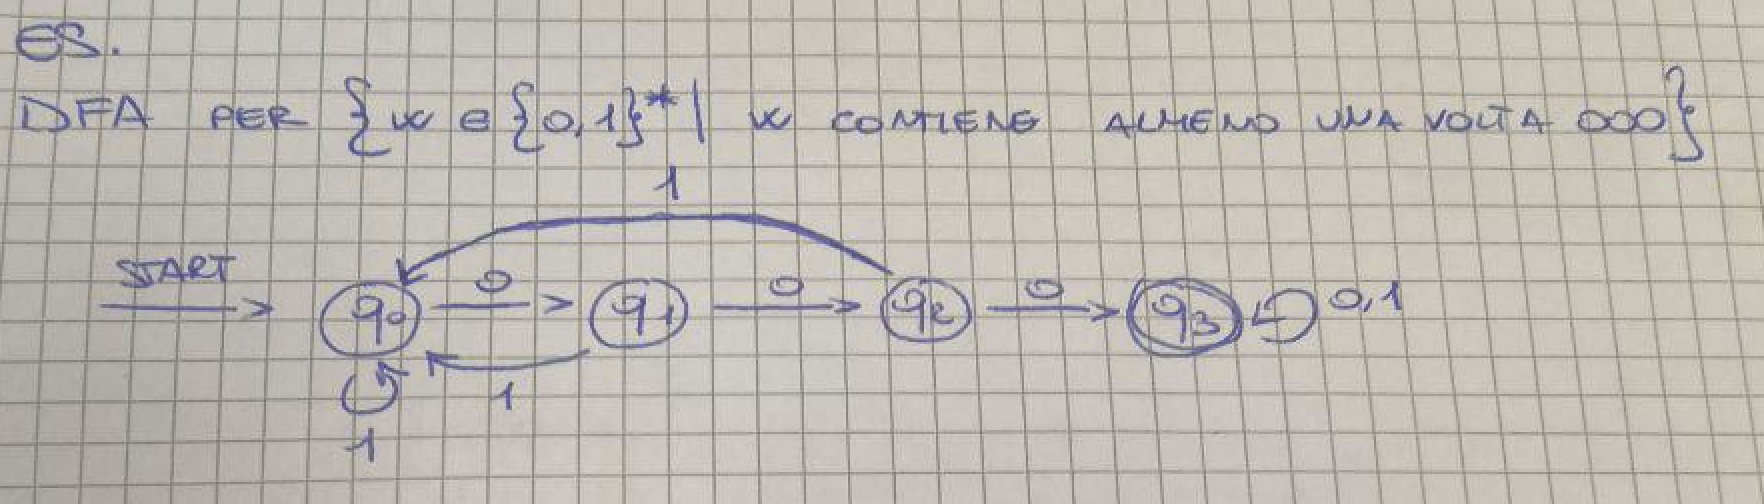
\includegraphics[width=0.75\textwidth]{16}
\end{center}
\paragraph{Esercizio 14: }
Progettare un DFA per L = $\{w \in \{0,1\}^{*}$ | w \textbf{non} contiene
000\}
\begin{center}
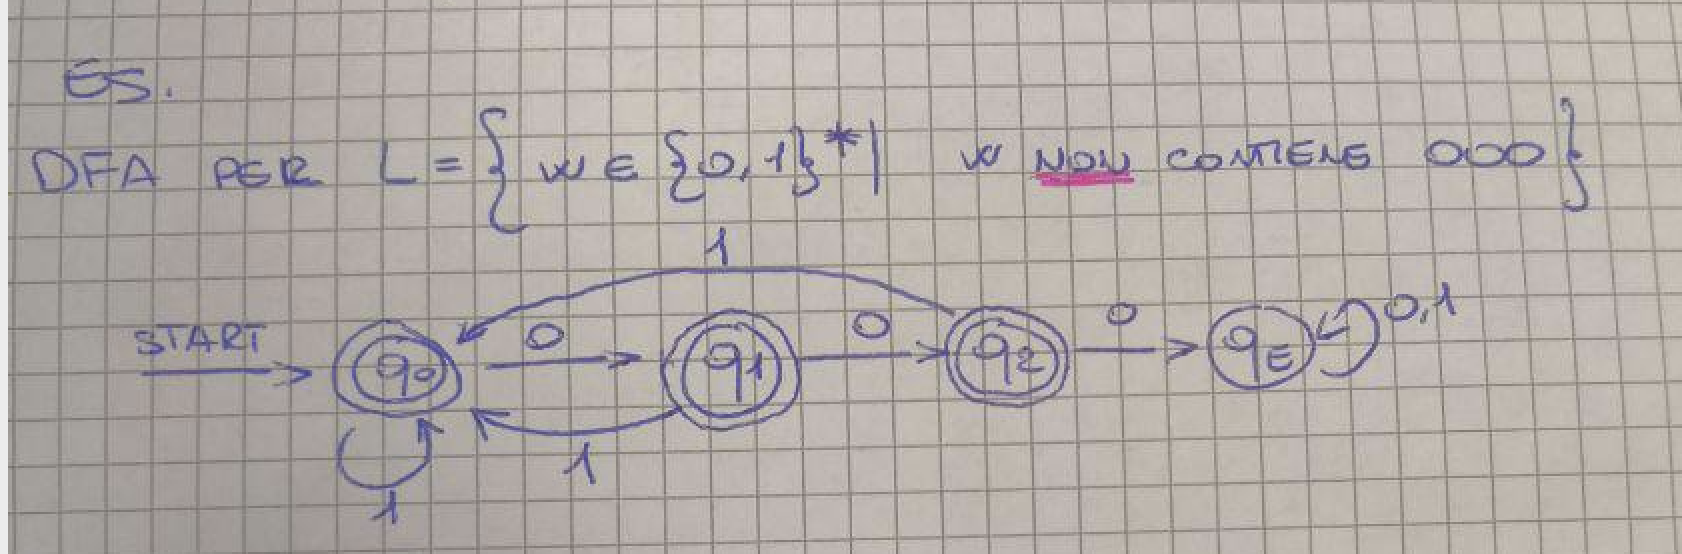
\includegraphics[width=0.75\textwidth]{17}
\end{center}
Dato un linguaggio ed un automa per esso, per capire come fare il complemento (
tutte le stringhe che NON appartengono al linguaggio) osserviamo il modo in cui
differiscono i due esercizi precedenti 
\paragraph{Esercizio 15: }
Progettare un DFA per L = $\{w \in \{0,1\}^{*}$ | w contiene esattamente una volta
000\}
\begin{center}
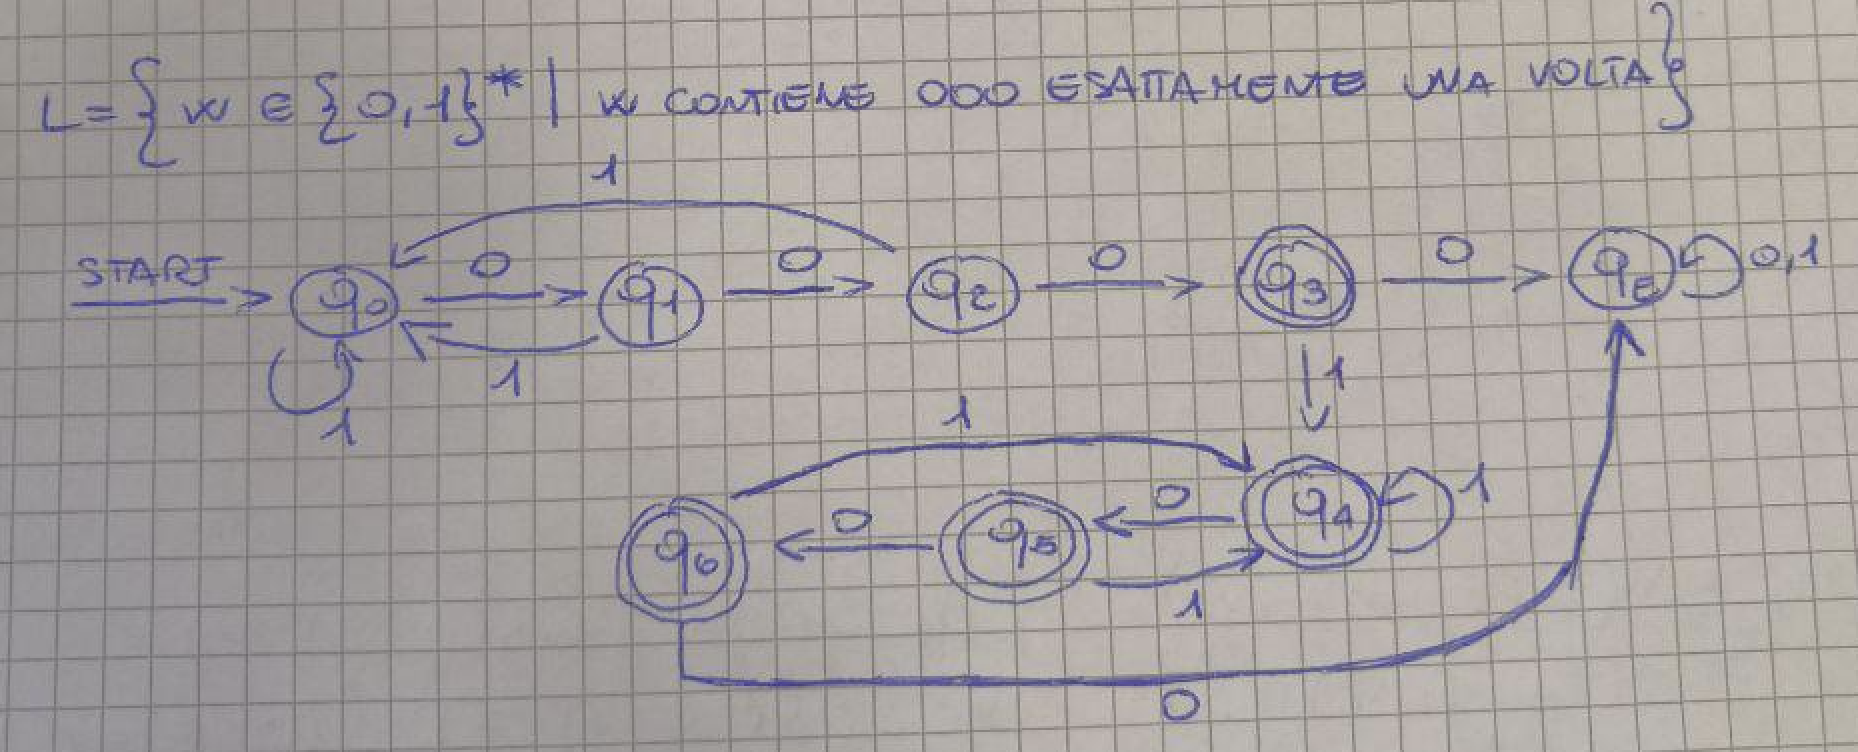
\includegraphics[width=0.75\textwidth]{18}
\end{center}
\paragraph{Esercizio 16: }
Progettare un DFA per L =$ \{w \in \{a,b,c\}^{*}$ | w finisce con b e le occorrenze
di b sono singole o a coppie\}
\begin{center}
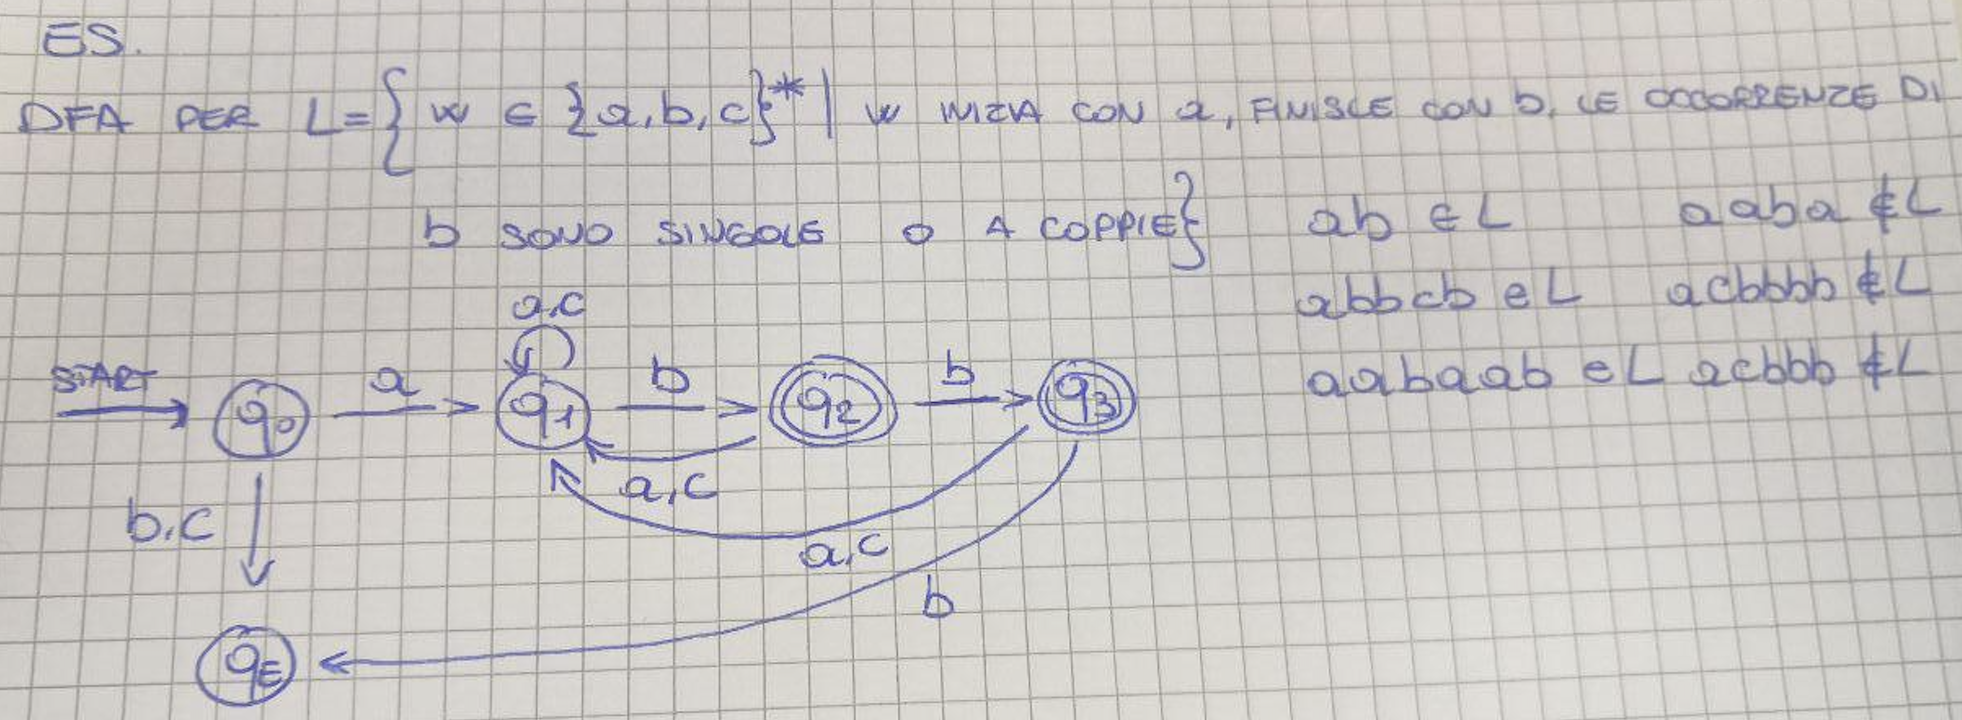
\includegraphics[width=0.75\textwidth]{19}
\end{center}
\section{Automa a stati finiti NON deterministico: NFA}
Per introdurci a questo argomento, vediamo un esercizio:
\paragraph{Esercizio 17: }
Progettare un DFA per L = \{x01 | x$\in\{0,1\}^{*}$\}
\begin{center}
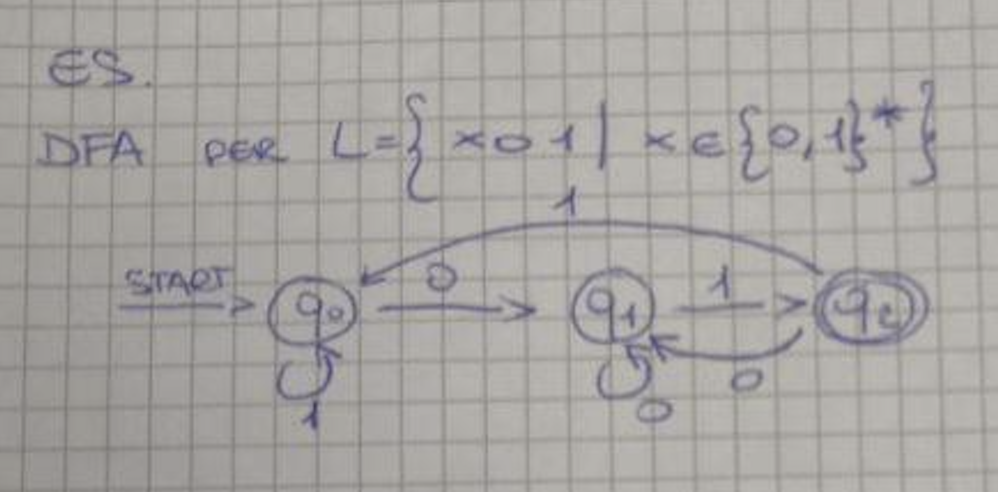
\includegraphics[width=0.75\textwidth]{20}
\end{center}
In caso di automi complicati potrebbero verificarsi sviste, problemi o errori, 
pertanto sono stati inventati gli automi a stati finiti \textbf{NON} deterministici.
\\ \\
Nei DFA $\delta$ prende lo stato in cui si trova l'automa, prende l'input e dice
cosa diventerà quello stato MENTRE nell'NFA $\delta$ guarda cosa entra e poi 
ci indirizza ad un certo insieme di stati:
\[
\delta : Q \times \Sigma \to 2^{Q}
\]
\begin{center}
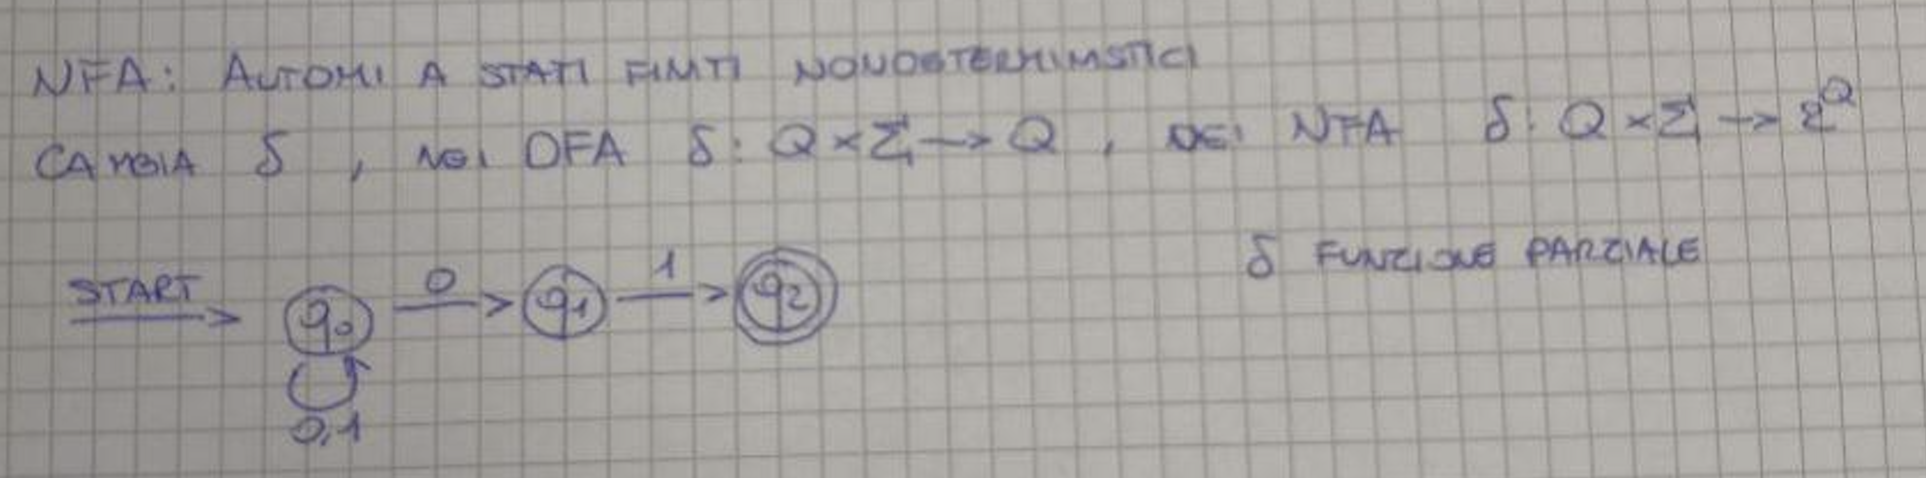
\includegraphics[width=0.75\textwidth]{21}
\end{center}
Come è possibile notare adesso $\delta$ è diventata una funzione parziale, inoltre
il non determinismo è visibile in due modi:
\begin{enumerate}
	\item Trovo tutte le possibilità, cioè l'automa si trova in più stati 
	contemporaneamente, si spezza, si duplica, ed una parte continua con una
	sua computazione, l'altra con la sua. 
	\begin{center}
	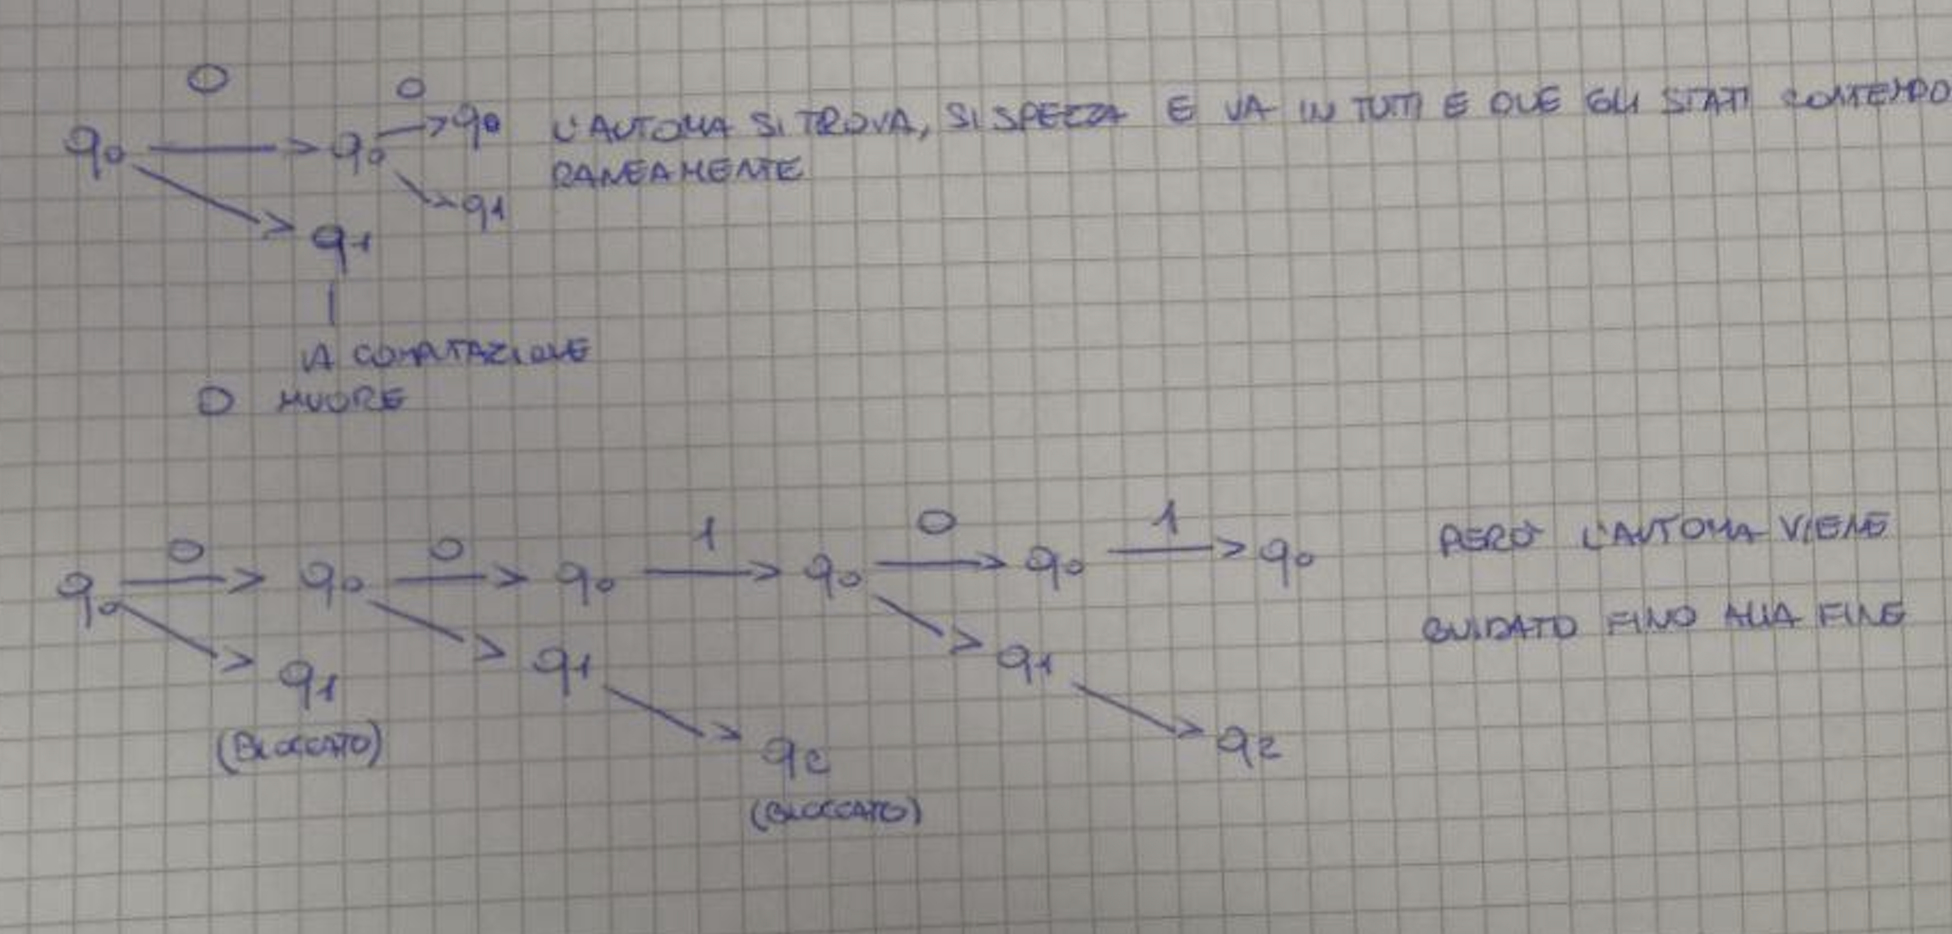
\includegraphics[width=0.75\textwidth]{22}
	\end{center}
	\paragraph{Cosa notiamo? }Uno dei rami farà morire la coputazione, nel senso
	che letteralmente si blocca, non può proseguire, ma gli altri possono continuare.
\end{enumerate}
{\color{black} \rule{\linewidth}{0.3mm}}
\paragraph{Esercizio: }Dato L =\{$x01|x\in\{0,1\}^{\star}$\} 
Il DFA risulterebbe: 
\begin{center}
\begin{tikzpicture}[scale=0.2]
\tikzstyle{every node}+=[inner sep=0pt]
\draw [black] (13.5,-21.5) circle (3);
\draw (13.5,-21.5) node {$q0$};
\draw [black] (37.2,-20.2) circle (3);
\draw (37.2,-20.2) node {$q1$};
\draw [black] (55.5,-19.2) circle (3);
\draw (55.5,-19.2) node {$q2$};
\draw [black] (55.5,-19.2) circle (2.4);
\draw [black] (6.7,-25.8) -- (10.96,-23.1);
\draw (6.07,-27.1) node [left] {$start$};
\fill [black] (10.96,-23.1) -- (10.02,-23.11) -- (10.56,-23.95);
\draw [black] (16.455,-20.98) arc (98.98993:87.28939:87.21);
\fill [black] (34.21,-20.01) -- (33.43,-19.47) -- (33.38,-20.47);
\draw (25.24,-19.49) node [above] {$0$};
\draw [black] (52.843,-20.586) arc (-66.99585:-106.74854:18.926);
\fill [black] (52.84,-20.59) -- (51.91,-20.44) -- (52.3,-21.36);
\draw (46.54,-22.61) node [below] {$1$};
\draw [black] (14.823,-24.18) arc (54:-234:2.25);
\draw (13.5,-28.75) node [below] {$1$};
\fill [black] (12.18,-24.18) -- (11.3,-24.53) -- (12.11,-25.12);
\draw [black] (39.854,-18.807) arc (113.12545:73.13016:18.826);
\fill [black] (39.85,-18.81) -- (40.79,-18.95) -- (40.39,-18.03);
\draw (46.16,-16.77) node [above] {$0$};
\draw [black] (37.971,-23.087) arc (42.69007:-245.30993:2.25);
\draw (35.32,-27.41) node [below] {$0$};
\fill [black] (35.38,-22.57) -- (34.45,-22.74) -- (35.13,-23.48);
\draw [black] (54.072,-21.836) arc (-32.05375:-141.67726:23.813);
\fill [black] (15.21,-23.96) -- (15.31,-24.9) -- (16.1,-24.28);
\draw (35.25,-33.53) node [below] {$1$};
\end{tikzpicture}
\end{center}
Mentre l'NFA: $S:Q\times\Sigma \to 2^{Q}$ con $Q = \{a,b,c\}$ e
$2^{Q} = \{\varnothing, \{a\}, \{b\}, \{c\}, \{a,b\}, \{a,c\, \{b,c\},\{a,b,c\}\}$
\begin{center}
\begin{tikzpicture}[scale=0.2]
\tikzstyle{every node}+=[inner sep=0pt]
\draw [black] (16.8,-20.8) circle (3);
\draw (16.8,-20.8) node {$q0$};
\draw [black] (40.1,-20.9) circle (3);
\draw (40.1,-20.9) node {$q1$};
\draw [black] (64.6,-20.2) circle (3);
\draw (64.6,-20.2) node {$q2$};
\draw [black] (64.6,-20.2) circle (2.4);
\draw [black] (19.8,-20.81) -- (37.1,-20.89);
\fill [black] (37.1,-20.89) -- (36.3,-20.38) -- (36.3,-21.38);
\draw (28.45,-20.35) node [above] {$0$};
\draw [black] (43.045,-20.329) arc (99.68657:83.58658:66.376);
\fill [black] (61.63,-19.8) -- (60.89,-19.21) -- (60.78,-20.21);
\draw (52.3,-18.88) node [above] {$1$};
\draw [black] (8.1,-20.8) -- (13.8,-20.8);
\draw (7.6,-20.8) node [left] {$start$};
\fill [black] (13.8,-20.8) -- (13,-20.3) -- (13,-21.3);
\draw [black] (17.807,-23.614) arc (47.41806:-240.58194:2.25);
\draw (15.6,-28.16) node [below] {$0,1$};
\fill [black] (15.18,-23.31) -- (14.27,-23.56) -- (15.01,-24.24);
\end{tikzpicture}
\end{center}
Ora disegnamo la tabella:
\begin{center}
\begin{tabular}{ |c|c|c| } 
\hline
& 0 & 1 \\ \hline
q0 & \{q0,q1\} & \{q0\} \\ 
\hline
q1 & $\varnothing$ & \{q2\} \\
\hline
q2 & $\varnothing$ & $\varnothing$ \\ 
\hline
\end{tabular}
(Siccome non so come fare questo grafico, ringrazio di nuovo l'esistenza di Gaia)

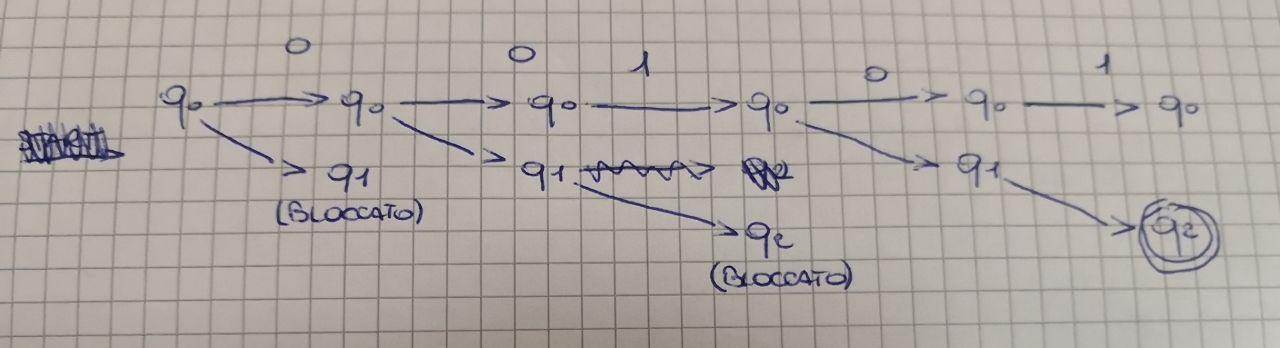
\includegraphics[width=0.75\textwidth]{23}
\end{center}
A questo punto come si sviluppa $\widehat{\delta}(q,w)?$ Che ci dice in quale 
stato si trova l'automa dopo aver consumato w. O meglio, in quale insieme di stati
si va a trovare.
\paragraph{$1^{a}$ definizione induttiva: }
\begin{center}
\begin{itemize}
	\item Base: $\widehat{\delta}(q,w) = \{q\} \forall q \in Q$
	\item Passo induttivo: posto $w = ax$, con $a \in \Sigma$ e $x \in 
	\Sigma^{\star}$ e $\delta(q,a) = \{p_{1}, p_{2}, ..., p_{x}\}$ ALLORA
	$\widehat{\delta} = \bigcup \limits_{i=1}^{k} \widehat{\delta}(p_{i},x) =
	\{r_{1}, r_{2}, ..., r_{m}\}$
\end{itemize}
\end{center}

\paragraph{$2^{a}$ definizione induttiva: }
\begin{center}
\begin{itemize}
	\item Base: $\widehat{\delta}(q,w) = \{q\} \forall q \in Q$
	\item Passo induttivo: posto $w = xa$, con $a \in \Sigma$ e $x \in 
	\Sigma^{\star}$ e $\delta(q,x) = \{p_{1}, p_{2}, ..., p_{x}\}$ ALLORA
	$\widehat{\delta} = \bigcup \limits_{i=1}^{k} \widehat{\delta}(p_{i},a) =
	\{r_{1}, r_{2}, ..., r_{m}\}$
\end{itemize}
\end{center}
(Per farla in breve, è identica MA si invertono la x e la a.)
\paragraph{Esempio: }Data la stringa w = 00101, \\
$\widehat{\delta}(q_{0}, \epsilon) = \{q_{0}\}$, \\
$\widehat{\delta}(q_{0}, 0) = \delta(q_{0},0) = \{q_{0}, q_{1}\}$, \\
$\widehat{\delta}(q_{0}, 00) = \delta(q_{0},0) \cup \delta(q_{1},0) = 
\{q_{0},q_{1}\cup \varnothing\} = \{q_{0},q_{1}\}$\\
$\widehat{\delta}(q_{0}, 001) = \delta(q_{0},1) \cup \delta(q_{1},1) = 
\{q_{0}\} \cup \{q_{2}\} = \{q_{0}, q_{2}\}$ \\
$\widehat{\delta}(q_{0}, 0010) = \delta(q_{0},0) \cup \delta(q_{2},0) =
\{q_{0},q_{1}\}\cup \varnothing = \{q_{0},q_{1}\}$ \\
$\widehat{\delta}(q_{0}, 00101) = \delta(q_{0}, 1) \cup \delta(q_{1},1) =
\{q_{0}\}\cup \{q_{2}\} = \{q_{0}, q_{2}\}$ \\
Dato che $q_{2}$ è stato accettante, ovvero appartiene all'insieme degli stati finali
la stringa w = 00101 è accettata dall'automa (NFA)
\section{Linguaggio accettato}
\paragraph{Definizione: }Sia A = (Q, $\Sigma, \delta, q_{0}$, F) un NFA, il 
linguaggio accettato da A è 
\[
L(A)=\{w\in \Sigma^{\star} | \widehat{\delta}(q_{0},w \cap F \neq \varnothing\}
\]
\section{Trasformazione da NFA a DFA}
Per ogni NFA esiste un DFA in grado di simularlo:
\paragraph{Definizione: }Dato un NFA N = ($Q_{N}, \Sigma, \delta_{N},q_{0}, F_{N}$)
costruiamo un DFA D = ($Q_{D},\Sigma, \delta_{D},\{q_{0}\}, F_{D}$)
Però occhio, la presenza di $q_{0}$ dovrebbe violare la definizione di DFA, 
pertanto possiamo pure chiamarlo Pippo, possiamo rinominarlo come ci pare. 
Questo insieme che vediamo come $q_{0}$, il DFA lo vede come entità/oggetto 
indivisibile TALE CHE L(D) = L(N) (costruzione per sottoinsiemi) %lolololol <3
\subparagraph{Com'è fatto $Q_{D}$?} E' l'insieme della parti di $Q_{N}$, ossia $2^{Q_{N}}$
\subparagraph{Com'è fatto $F_{D}$?} $F_{D}$ = \{$S \subseteq Q_{N}|S\cap F_{n}\neq 
\varnothing$\}	
\subparagraph{Com'è fatta $\delta_{D}$?} $\forall S \subseteq Q_{N}$ e $\forall a \in \Sigma$
$\delta_{D}(S,a) = \bigcup \limits_{p \in S} \delta_{N}(p,a)$	
\paragraph{Riprendiamo l'automa di prima: }
\begin{center}
\begin{tikzpicture}[scale=0.2]
\tikzstyle{every node}+=[inner sep=0pt]
\draw [black] (16.8,-20.8) circle (3);
\draw (16.8,-20.8) node {$q0$};
\draw [black] (40.1,-20.9) circle (3);
\draw (40.1,-20.9) node {$q1$};
\draw [black] (64.6,-20.2) circle (3);
\draw (64.6,-20.2) node {$q2$};
\draw [black] (64.6,-20.2) circle (2.4);
\draw [black] (19.8,-20.81) -- (37.1,-20.89);
\fill [black] (37.1,-20.89) -- (36.3,-20.38) -- (36.3,-21.38);
\draw (28.45,-20.35) node [above] {$0$};
\draw [black] (43.045,-20.329) arc (99.68657:83.58658:66.376);
\fill [black] (61.63,-19.8) -- (60.89,-19.21) -- (60.78,-20.21);
\draw (52.3,-18.88) node [above] {$1$};
\draw [black] (8.1,-20.8) -- (13.8,-20.8);
\draw (7.6,-20.8) node [left] {$start$};
\fill [black] (13.8,-20.8) -- (13,-20.3) -- (13,-21.3);
\draw [black] (17.807,-23.614) arc (47.41806:-240.58194:2.25);
\draw (15.6,-28.16) node [below] {$0,1$};
\fill [black] (15.18,-23.31) -- (14.27,-23.56) -- (15.01,-24.24);
\end{tikzpicture}
\end{center}
\begin{center}
\begin{tabular}{ |c|c|c| } 
\hline
\_ & 0 & 1  \\ 
$\varnothing$ & $\varnothing$ & $\varnothing$\\ 
$ \to{q_{0}}$ & \{$q_{0}, q_{1}$\} &  \{$q_{0}$\}  \\ 
$\{q_{1}\}$ & $\varnothing$  &  \{$q_{2}$\}     \\ 
$\{q_{2}\}$ & $\varnothing $ &   $\varnothing  $  \\ 
$\{q_{0}, q_{1}\}$ & $\{q_{0}, q_{1}\} $ &   $\{q_{0}, q_{2}\}$    \\ 
$\star\{q_{0}, q_{2}\} $& $\{q_{0}, q_{1}\}$ & $ \{q_{0}\}$ \\ 
$\star\{q_{1}, q_{2}\} $& $\varnothing \cup \varnothing $& $ \{q_{2}\} $ \\
$\star\{q_{0}, q_{1}, q_{2}\} $& $\{q_{0}, q_{1}\}$ &  $ \{q_{0}, q_{2}\}$    \\  
\hline
\end{tabular}
\end{center}
\begin{center}
\begin{tabular}{ |c|c|c| } 
\hline
A & A & A \\ 
B & E & B \\ 
C & A & D \\ 
D & A & A \\ 
E & E & F \\ 
F & E & B \\ 
G & A & D \\ 
H & E & F \\
\hline
\end{tabular}
\end{center}
Contiamo che $S_{D}(\{q_{0},q_{1}\}, 0) = \delta_{N}(q_{0},0) \cup \delta_{N}(q_{1},0)
= \{q_{0},q_{1} \cup \varnothing = \{q_{0}, q_{1}\}\}$ 
Ecco il DFA che ne risulterebbe:
\begin{center}
\begin{tikzpicture}[scale=0.2]
\tikzstyle{every node}+=[inner sep=0pt]
\draw [black] (19.9,-22.5) circle (3);
\draw (19.9,-22.5) node {$A$};
\draw [black] (16.7,-32.9) circle (3);
\draw (16.7,-32.9) node {$B$};
\draw [black] (35.5,-33.2) circle (3);
\draw (35.5,-33.2) node {$E$};
\draw [black] (33,-8.7) circle (3);
\draw (33,-8.7) node {$C$};
\draw [black] (55.2,-8.1) circle (3);
\draw (55.2,-8.1) node {$D$};
\draw [black] (55.2,-8.1) circle (2.4);
\draw [black] (58.3,-33.5) circle (3);
\draw (58.3,-33.5) node {$F$};
\draw [black] (58.3,-33.5) circle (2.4);
\draw [black] (51.5,-20.5) circle (3);
\draw (51.5,-20.5) node {$G$};
\draw [black] (46.7,-48.6) circle (3);
\draw (46.7,-48.6) node {$H$};
\draw [black] (46.7,-48.6) circle (2.4);
\draw [black] (20.703,-19.621) arc (192.15438:-95.84562:2.25);
\draw (26.17,-16.98) node [above] {$0,1$};
\fill [black] (22.67,-21.39) -- (23.56,-21.71) -- (23.35,-20.73);
\draw [black] (6.1,-32.9) -- (13.7,-32.9);
\draw (5.6,-32.9) node [left] {$Start$};
\fill [black] (13.7,-32.9) -- (12.9,-32.4) -- (12.9,-33.4);
\draw [black] (17.522,-35.773) arc (43.69515:-244.30485:2.25);
\draw (15,-40.13) node [below] {$1$};
\fill [black] (14.92,-35.3) -- (14,-35.49) -- (14.69,-36.21);
\draw [black] (19.7,-32.95) -- (32.5,-33.15);
\fill [black] (32.5,-33.15) -- (31.71,-32.64) -- (31.69,-33.64);
\draw [black] (19.589,-19.525) arc (-181.60736:-265.41138:11.335);
\fill [black] (19.59,-19.52) -- (20.11,-18.74) -- (19.11,-18.71);
\draw (22.17,-10.57) node [left] {$0$};
\draw [black] (52.998,-10.137) arc (-48.93661:-86.67915:50.253);
\fill [black] (22.9,-22.42) -- (23.73,-22.87) -- (23.67,-21.87);
\draw (40.65,-19.31) node [below] {$0,1$};
\draw [black] (36,-8.62) -- (52.2,-8.18);
\fill [black] (52.2,-8.18) -- (51.39,-7.7) -- (51.41,-8.7);
\draw (44.12,-8.93) node [below] {$1$};
\draw [black] (36.823,-35.88) arc (54:-234:2.25);
\draw (35.5,-40.45) node [below] {$0$};
\fill [black] (34.18,-35.88) -- (33.3,-36.23) -- (34.11,-36.82);
\draw [black] (38.009,-31.561) arc (118.45654:60.03576:18.266);
\fill [black] (55.84,-31.8) -- (55.39,-30.96) -- (54.89,-31.83);
\draw (46.96,-28.84) node [above] {$1$};
\draw [black] (55.436,-34.388) arc (-75.4292:-106.0785:32.346);
\fill [black] (38.34,-34.16) -- (38.97,-34.87) -- (39.25,-33.9);
\draw (46.87,-35.94) node [below] {$0$};
\draw [black] (61.13,-34.46) arc (99:-189:2.25);
\draw (63.6,-39.75) node [right] {$1$};
\fill [black] (59.26,-36.33) -- (58.89,-37.2) -- (59.88,-37.04);
\draw [black] (52.36,-17.63) -- (54.34,-10.97);
\fill [black] (54.34,-10.97) -- (53.63,-11.6) -- (54.59,-11.88);
\draw (54.12,-14.9) node [right] {$1$};
\draw [black] (48.81,-21.827) arc (-66.02561:-106.73142:37.56);
\fill [black] (22.74,-23.48) -- (23.36,-24.19) -- (23.65,-23.23);
\draw (36,-25.55) node [below] {$0$};
\draw [black] (44.94,-46.17) -- (37.26,-35.63);
\fill [black] (37.26,-35.63) -- (37.33,-36.57) -- (38.14,-35.98);
\draw (41.69,-39.52) node [right] {$0$};
\draw [black] (48.53,-46.22) -- (56.47,-35.88);
\fill [black] (56.47,-35.88) -- (55.59,-36.21) -- (56.38,-36.82);
\draw (53.07,-42.46) node [right] {$1$};
\end{tikzpicture}
\end{center}
\paragraph{Come si nota è davvero complesso: }
In realtà avremmo dovuto calcolare solo B E ed F, perchè alcuni stati non sono
nemmeno raggiungibili, quindi non avremmo dovuto iniziare indicando tutti i
possibili sottoinsiemi MA considerare il tutto stato per stato:
\begin{center}
\begin{tabular}{ |c|c|c| } 
\hline
\_ & 0 & 1 \\
\hline
$\to\{q_{0}\} $&$ \{q_{0},q_{1}\}$ & $\{q_{0}\} $\\ 
$\{q_{0},q_{1}\} $&$\{q_{0},q_{1}\}$ & $\{q_{0},q_{2}\}$ \\ 
$\star\{q_{0},q_{2}\}$ &$ \{q_{0},q_{1}\}$ & $\{q_{0}\} $\\
\hline
\end{tabular}
\end{center}
\begin{center}
\begin{tabular}{ |c|c|c| } 
\hline
B & E & B \\
E & E & F \\ 
F & E & B \\ 
\hline
\end{tabular}
\end{center}
\paragraph{Altro esempio: }Dato il seguente NFA:

\begin{center}
\begin{tikzpicture}[scale=0.2]
\tikzstyle{every node}+=[inner sep=0pt]
\draw [black] (16.5,-23.6) circle (3);
\draw (16.5,-23.6) node {$q0$};
\draw [black] (16.5,-23.6) circle (2.4);
\draw [black] (36.6,-14.7) circle (3);
\draw (36.6,-14.7) node {$q1$};
\draw [black] (36.6,-14.7) circle (2.4);
\draw [black] (52.1,-22.9) circle (3);
\draw (52.1,-22.9) node {$q3$};
\draw [black] (36.5,-36) circle (3);
\draw (36.5,-36) node {$q2$};
\draw [black] (9.3,-24.8) -- (13.54,-24.09);
\draw (8.59,-25.03) node [left] {$start$};
\fill [black] (13.54,-24.09) -- (12.67,-23.73) -- (12.83,-24.72);
\draw [black] (19.24,-22.39) -- (33.86,-15.91);
\fill [black] (33.86,-15.91) -- (32.92,-15.78) -- (33.33,-16.7);
\draw (27.47,-19.66) node [below] {$a$};
\draw [black] (19.05,-25.18) -- (33.95,-34.42);
\fill [black] (33.95,-34.42) -- (33.53,-33.57) -- (33.01,-34.42);
\draw (25.56,-30.3) node [below] {$a$};
\draw [black] (35.098,-33.351) arc (-156.43853:-204.09946:19.82);
\fill [black] (35.17,-17.34) -- (34.39,-17.86) -- (35.3,-18.27);
\draw (32.94,-25.34) node [left] {$b$};
\draw [black] (38.118,-17.284) arc (25.76586:-26.30385:18.394);
\fill [black] (38.04,-33.43) -- (38.85,-32.94) -- (37.95,-32.49);
\draw (40.45,-25.37) node [right] {$a$};
\draw [black] (36.552,-11.712) arc (208.65382:-79.34618:2.25);
\draw (40.42,-8.09) node [above] {$a$};
\fill [black] (38.94,-12.84) -- (39.88,-12.9) -- (39.4,-12.02);
\draw [black] (51.094,-25.722) arc (-24.48568:-75.47103:17.658);
\fill [black] (51.09,-25.72) -- (50.31,-26.24) -- (51.22,-26.66);
\draw (47.39,-32.42) node [below] {$b$};
\draw [black] (49.8,-24.83) -- (38.8,-34.07);
\fill [black] (38.8,-34.07) -- (39.73,-33.94) -- (39.09,-33.17);
\draw (43.35,-28.96) node [above] {$a$};
\draw [black] (49.45,-21.5) -- (39.25,-16.1);
\fill [black] (39.25,-16.1) -- (39.73,-16.92) -- (40.19,-16.04);
\draw (45.29,-18.3) node [above] {$a$};
\end{tikzpicture}
\end{center}
\begin{center}
\begin{tabular}{ |c|c|c| } 
\hline
& a & b \\
\hline
$\star \to \{q_{0}\}$& $\{q_{0},q_{2}\}$ & $ \varnothing$\\ 
$\star\{q_{1},q_{2}\} $& $\{q_{1},q_{2}\} $&$ \{q_{1},q_{3}\}$ \\ 
$ \varnothing $& $\varnothing$ & $\varnothing$ \\ 
$\star\{q_{1},q_{3}\} $& $\{q_{1},q_{2}\} $& $\varnothing$\\ 
\hline
\end{tabular}
\end{center}
Ecco il risultato della conversione in DFA: 
\begin{center}
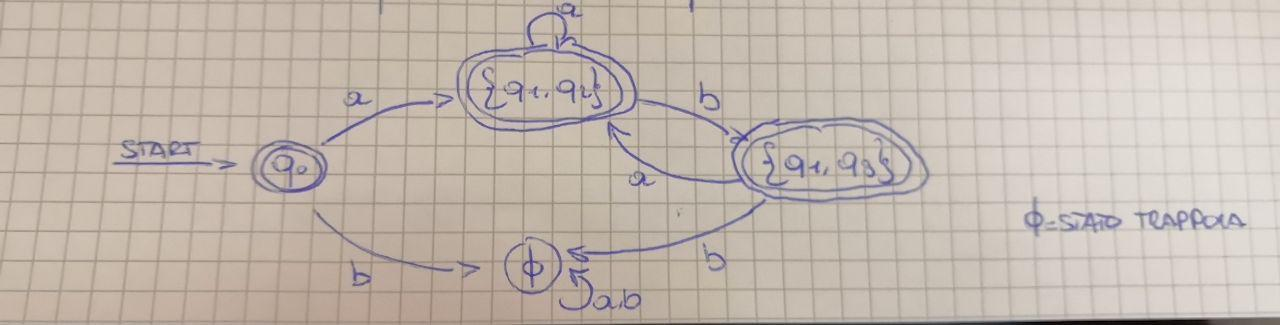
\includegraphics[width=0.75\textwidth]{24}
\end{center}
Come è possibile notare, è stato usato invece delle letterine dell'alfabeto tanto
carine, la dicitura con gli insiemi, che è brutta e cattiva. E non perchè sono
completamente incapace di fare le parentesi graffe, lo giuro.
\subparagraph{Scherzi a parte,}	 Una scrittura, si 
equivale all'altra
\paragraph{Precisazione: }Se l'NFA si trova in uno stato q e se riceve un 
carattere 'a' finisce in due stati p ed r allora il DFA risulta che quando
lo stato \{$q_{0}$\} riceve per l'aoppunto 'a' allora si ottiene lo stato \{p,a\}
\paragraph{Osservazione: }Si nota che $|Q_{N}| = n \implies |Q_{D}| = 2^{N}$,
ad esempio:

\begin{center}
\begin{tikzpicture}[scale=0.2]
\tikzstyle{every node}+=[inner sep=0pt]
\draw [black] (14.4,-31.2) circle (3);
\draw (14.4,-31.2) node {$q0$};
\draw [black] (29.7,-31.2) circle (3);
\draw (29.7,-31.2) node {$q1$};
\draw [black] (42.4,-31.2) circle (3);
\draw (42.4,-31.2) node {$q2$};
\draw [black] (63,-47) circle (3);
\draw (63,-47) node {$q(n-1)$};
\draw [black] (68.3,-29.7) circle (3);
\draw (68.3,-29.7) node {$qn$};
\draw [black] (68.3,-29.7) circle (2.4);
\draw [black] (53.9,-29.8) circle (3);
\draw (53.9,-29.8) node {$...$};
\draw [black] (13.077,-28.52) arc (234:-54:2.25);
\draw (14.4,-23.95) node [above] {$0,1$};
\fill [black] (15.72,-28.52) -- (16.6,-28.17) -- (15.79,-27.58);
\draw [black] (6,-34.4) -- (11.6,-32.27);
\draw (5.25,-35.23) node [left] {$start$};
\fill [black] (11.6,-32.27) -- (10.67,-32.09) -- (11.03,-33.02);
\draw [black] (17.4,-31.2) -- (26.7,-31.2);
\fill [black] (26.7,-31.2) -- (25.9,-30.7) -- (25.9,-31.7);
\draw (22.05,-31.7) node [below] {$1$};
\draw [black] (32.7,-31.2) -- (39.4,-31.2);
\fill [black] (39.4,-31.2) -- (38.6,-30.7) -- (38.6,-31.7);
\draw (36.05,-31.7) node [below] {$0,1$};
\draw [black] (63.88,-44.13) -- (67.42,-32.57);
\fill [black] (67.42,-32.57) -- (66.71,-33.19) -- (67.66,-33.48);
\draw (66.42,-38.97) node [right] {$0,1$};
\draw [black] (45.38,-30.84) -- (50.92,-30.16);
\fill [black] (50.92,-30.16) -- (50.07,-29.76) -- (50.19,-30.76);
\draw (48.62,-31.16) node [below] {$0,1$};
\draw [black] (55.3,-32.45) -- (61.6,-44.35);
\fill [black] (61.6,-44.35) -- (61.66,-43.41) -- (60.78,-43.87);
\draw (57.77,-39.56) node [left] {$0,1$};
\end{tikzpicture}
\end{center}
L = \{$w\in \{0,1\}^{\star}|$ è l'n-esimo simbolo di w dalla fine è 1\}
\begin{center}
\begin{tikzpicture}[scale=0.2]
\tikzstyle{every node}+=[inner sep=0pt]
\draw [black] (10.7,-25.5) circle (3);
\draw (10.7,-25.5) node {$1$};
\draw [black] (19.9,-19.5) circle (3);
\draw (19.9,-19.5) node {$2$};
\draw [black] (31.4,-19.1) circle (3);
\draw (31.4,-19.1) node {$3$};
\draw [black] (43,-18.9) circle (3);
\draw (43,-18.9) node {$4$};
\draw [black] (43,-18.9) circle (2.4);
\draw [black] (20.7,-32.3) circle (3);
\draw (20.7,-32.3) node {$5$};
\draw [black] (34.8,-32.3) circle (3);
\draw (34.8,-32.3) node {$6$};
\draw [black] (48.2,-31.4) circle (3);
\draw (48.2,-31.4) node {$7$};
\draw [black] (60,-31.3) circle (3);
\draw (60,-31.3) node {$8$};
\draw [black] (60,-31.3) circle (2.4);
\draw [black] (6.5,-33.9) -- (9.36,-28.18);
\draw (4.3,-34.41) node [below] {$start$};
\fill [black] (9.36,-28.18) -- (8.55,-28.68) -- (9.45,-29.12);
\draw [black] (13.21,-23.86) -- (17.39,-21.14);
\fill [black] (17.39,-21.14) -- (16.44,-21.16) -- (16.99,-21.99);
\draw (16.52,-23) node [below] {$w$};
\draw [black] (22.9,-19.4) -- (28.4,-19.2);
\fill [black] (28.4,-19.2) -- (27.58,-18.73) -- (27.62,-19.73);
\draw (25.67,-19.83) node [below] {$e$};
\draw [black] (34.4,-19.05) -- (40,-18.95);
\fill [black] (40,-18.95) -- (39.19,-18.47) -- (39.21,-19.47);
\draw (37.21,-19.52) node [below] {$b$};
\draw [black] (13.18,-27.19) -- (18.22,-30.61);
\fill [black] (18.22,-30.61) -- (17.84,-29.75) -- (17.28,-30.58);
\draw (14.75,-29.4) node [below] {$e$};
\draw [black] (23.7,-32.3) -- (31.8,-32.3);
\fill [black] (31.8,-32.3) -- (31,-31.8) -- (31,-32.8);
\draw (27.75,-32.8) node [below] {$b$};
\draw [black] (37.79,-32.1) -- (45.21,-31.6);
\fill [black] (45.21,-31.6) -- (44.38,-31.16) -- (44.44,-32.15);
\draw (41.59,-32.41) node [below] {$a$};
\draw [black] (51.2,-31.37) -- (57,-31.33);
\fill [black] (57,-31.33) -- (56.2,-30.83) -- (56.2,-31.83);
\draw (54.1,-31.86) node [below] {$y$};
\draw [black] (8.376,-23.621) arc (258.77514:-29.22486:2.25);
\draw (6.78,-18.86) node [above] {$\Sigma$};
\fill [black] (10.78,-22.51) -- (11.42,-21.83) -- (10.44,-21.63);
\end{tikzpicture}
\end{center}
Da questo automa si può notare che esista una corrispondenza tra "web" ed "ebay"
E $\Sigma = {a,b,c,....,z}$. Se avessimo provato a fare questo da un DFA sarebbe
stato davvero più complesso
\chapter{$\epsilon$ NFA}
Sono un'estensione dell'NFA in cui si includono le $\epsilon$-transizioni e le
$\epsilon$-mosse

\section{$\epsilon$-mossa}
E' una trasmissione spontanea in cui l'automa cambia stato senza consumare il 
simbolo di input ricevuto.
\paragraph{Più precisamente: }$\epsilon-$NFA = ($Q,\Sigma,\delta, q_{2},F$),
$S:Q\times(\Sigma\cup\{\epsilon\})\to 2^{Q}$
\paragraph{Esercizio 1: }  Dato il seguente NFA:
\begin{center}
\begin{tikzpicture}[scale=0.2]
\tikzstyle{every node}+=[inner sep=0pt]
\draw [black] (16.8,-20.9) circle (3);
\draw (16.8,-20.9) node {$p$};
\draw [black] (40,-15.8) circle (3);
\draw (40,-15.8) node {$q$};
\draw [black] (29.4,-34.7) circle (3);
\draw (29.4,-34.7) node {$r$};
\draw [black] (6.4,-22.3) -- (13.83,-21.3);
\draw (5.72,-22.45) node [left] {$start$};
\fill [black] (13.83,-21.3) -- (12.97,-20.91) -- (13.1,-21.9);
\draw [black] (14.287,-19.283) arc (264.96376:-23.03624:2.25);
\draw (12.38,-14.61) node [above] {$a$};
\fill [black] (16.56,-17.92) -- (17.12,-17.17) -- (16.13,-17.08);
\draw [black] (26.448,-34.202) arc (-106.01528:-169.18984:13.336);
\fill [black] (26.45,-34.2) -- (25.82,-33.5) -- (25.54,-34.46);
\draw (19.74,-31.84) node [left] {$c$};
\draw [black] (19.241,-19.159) arc (122.29791:82.49808:26.791);
\fill [black] (37.05,-15.24) -- (36.33,-14.64) -- (36.2,-15.63);
\draw (27.18,-15.06) node [above] {$b$};
\draw [black] (37.209,-16.899) arc (-69.82177:-85.38224:65.854);
\fill [black] (19.79,-20.73) -- (20.63,-21.16) -- (20.55,-20.16);
\draw (29.23,-19.98) node [below] {$\epsilon$};
\draw [black] (40.223,-18.788) arc (-0.66181:-57.90967:17.405);
\fill [black] (32.07,-33.33) -- (33.01,-33.33) -- (32.48,-32.48);
\draw (38.66,-28.31) node [right] {$b$};
\draw [black] (30.87,-32.08) -- (38.53,-18.42);
\fill [black] (38.53,-18.42) -- (37.71,-18.87) -- (38.58,-19.36);
\draw (35.36,-26.46) node [right] {$\epsilon$};
\draw [black] (40.029,-12.812) arc (207.17419:-80.82581:2.25);
\draw (43.98,-9.27) node [above] {$a$};
\fill [black] (42.39,-14.01) -- (43.33,-14.08) -- (42.87,-13.2);
\draw [black] (30.435,-37.503) arc (47.99099:-240.00901:2.25);
\draw (28.5,-41.99) node [below] {$a$};
\fill [black] (27.8,-37.23) -- (26.9,-37.49) -- (27.64,-38.16);
\draw [black] (19.393,-22.405) arc (56.61574:28.17913:26.396);
\fill [black] (28.14,-31.98) -- (28.2,-31.04) -- (27.32,-31.51);
\draw (24.9,-25.19) node [right] {$c$};
\end{tikzpicture}
\end{center}
$\Sigma$ = \{a,b,c\}, se w = abac allora: \\
Partiamo dalla p e cerchiamo di capire dove si va a finire, ma in questo caso
c'è l'$\epsilon$-mossa, ti consente di o consumare un carattere per poi passare
ad un altro stato.
\subparagraph{All'atto pratico: }Da q posso andare in r consumando la 'b' oppure
con $\epsilon$-mossa posso andare in p senza consumare il carattere 	  
\paragraph{Esercizio 2: }
Riprendendo l'esempio dell'automa di E-Bay, questo è ciò che ne verrebbe fuori 
SE si aggiungono le mosse $\epsilon$:

\begin{center}
\begin{tikzpicture}[scale=0.2]
\tikzstyle{every node}+=[inner sep=0pt]
\draw [black] (18.3,-23.7) circle (3);
\draw (18.3,-23.7) node {$9$};
\draw [black] (30.2,-13) circle (3);
\draw (30.2,-13) node {$1$};
\draw [black] (45.4,-13.3) circle (3);
\draw (45.4,-13.3) node {$2$};
\draw [black] (59.2,-12.9) circle (3);
\draw (59.2,-12.9) node {$3$};
\draw [black] (71.6,-12.9) circle (3);
\draw (71.6,-12.9) node {$4$};
\draw [black] (71.6,-12.9) circle (2.4);
\draw [black] (30.2,-30.9) circle (3);
\draw (30.2,-30.9) node {$0$};
\draw [black] (42.5,-30.9) circle (3);
\draw (42.5,-30.9) node {$5$};
\draw [black] (55.3,-30.9) circle (3);
\draw (55.3,-30.9) node {$6$};
\draw [black] (65.2,-30.9) circle (3);
\draw (65.2,-30.9) node {$7$};
\draw [black] (74.8,-30.9) circle (3);
\draw (74.8,-30.9) node {$8$};
\draw [black] (74.8,-30.9) circle (2.4);
\draw [black] (7.5,-23.7) -- (15.3,-23.7);
\draw (7,-23.7) node [left] {$start$};
\fill [black] (15.3,-23.7) -- (14.5,-23.2) -- (14.5,-24.2);
\draw [black] (15.877,-21.95) arc (261.89727:-26.10273:2.25);
\draw (14.04,-17.23) node [above] {$\Sigma$};
\fill [black] (18.22,-20.71) -- (18.82,-19.99) -- (17.83,-19.85);
\draw [black] (15.877,-21.95) arc (261.89727:-26.10273:2.25);
\fill [black] (18.22,-20.71) -- (18.82,-19.99) -- (17.83,-19.85);
\draw [black] (20.53,-21.69) -- (27.97,-15.01);
\fill [black] (27.97,-15.01) -- (27.04,-15.17) -- (27.71,-15.91);
\draw (25.21,-18.84) node [below] {$\epsilon$};
\draw [black] (33.2,-13.06) -- (42.4,-13.24);
\fill [black] (42.4,-13.24) -- (41.61,-12.73) -- (41.59,-13.72);
\draw (37.79,-13.67) node [below] {$w$};
\draw [black] (48.4,-13.21) -- (56.2,-12.99);
\fill [black] (56.2,-12.99) -- (55.39,-12.51) -- (55.42,-13.51);
\draw (52.32,-13.63) node [below] {$e$};
\draw [black] (62.2,-12.9) -- (68.6,-12.9);
\fill [black] (68.6,-12.9) -- (67.8,-12.4) -- (67.8,-13.4);
\draw (65.4,-13.4) node [below] {$b$};
\draw [black] (20.87,-25.25) -- (27.63,-29.35);
\fill [black] (27.63,-29.35) -- (27.21,-28.51) -- (26.69,-29.36);
\draw (23.31,-27.8) node [below] {$\epsilon$};
\draw [black] (33.2,-30.9) -- (39.5,-30.9);
\fill [black] (39.5,-30.9) -- (38.7,-30.4) -- (38.7,-31.4);
\draw (36.35,-31.4) node [below] {$e$};
\draw [black] (45.5,-30.9) -- (52.3,-30.9);
\fill [black] (52.3,-30.9) -- (51.5,-30.4) -- (51.5,-31.4);
\draw (48.9,-31.4) node [below] {$b$};
\draw [black] (58.3,-30.9) -- (62.2,-30.9);
\fill [black] (62.2,-30.9) -- (61.4,-30.4) -- (61.4,-31.4);
\draw (60.25,-31.4) node [below] {$a$};
\draw [black] (68.2,-30.9) -- (71.8,-30.9);
\fill [black] (71.8,-30.9) -- (71,-30.4) -- (71,-31.4);
\draw (70,-31.4) node [below] {$y$};
\end{tikzpicture}
\end{center}
\paragraph{Esercizio 3: }Data ER = $a^{\star}b^{\star}c^{\star}$ e l'$\epsilon$-NFA:
\begin{center}
\begin{tikzpicture}[scale=0.2]
\tikzstyle{every node}+=[inner sep=0pt]
\draw [black] (11.3,-20.2) circle (3);
\draw (11.3,-20.2) node {$q0$};
\draw [black] (34.3,-19.9) circle (3);
\draw (34.3,-19.9) node {$q1$};
\draw [black] (57,-19.8) circle (3);
\draw (57,-19.8) node {$q2$};
\draw [black] (57,-19.8) circle (2.4);
\draw [black] (9.648,-17.71) arc (241.29521:-46.70479:2.25);
\draw (10.17,-12.92) node [above] {$a$};
\fill [black] (12.27,-17.37) -- (13.09,-16.91) -- (12.22,-16.43);
\draw [black] (14.3,-20.16) -- (31.3,-19.94);
\fill [black] (31.3,-19.94) -- (30.49,-19.45) -- (30.51,-20.45);
\draw (22.8,-20.56) node [below] {$\epsilon$};
\draw [black] (37.3,-19.89) -- (54,-19.81);
\fill [black] (54,-19.81) -- (53.2,-19.32) -- (53.2,-20.32);
\draw (45.65,-20.35) node [below] {$\epsilon$};
\draw [black] (32.478,-17.532) arc (245.30993:-42.69007:2.25);
\draw (32.42,-12.69) node [above] {$b$};
\fill [black] (35.07,-17.01) -- (35.86,-16.49) -- (34.95,-16.08);
\draw [black] (57.641,-16.881) arc (195.34019:-92.65981:2.25);
\draw (62.17,-14.03) node [above] {$c$};
\fill [black] (59.71,-18.53) -- (60.61,-18.8) -- (60.35,-17.84);
\draw [black] (5.5,-27.6) -- (9.45,-22.56);
\draw (3.27,-28.1) node [below] {$start$};
\fill [black] (9.45,-22.56) -- (8.56,-22.88) -- (9.35,-23.5);
\end{tikzpicture}
\end{center}
Andiamo a definire la $\epsilon$ chiusura, che per semplificare chiameremo 
ECLOSE(q) = insieme (ECLOSE Q $\to 2^{Q}$) degli stati raggiungibili da q 
tramite $\epsilon$-transizioni:
\subparagraph{Esempio: }	
\begin{center}
\begin{tikzpicture}[scale=0.2]
\tikzstyle{every node}+=[inner sep=0pt]
\draw [black] (12.5,-25.5) circle (3);
\draw (12.5,-25.5) node {$1$};
\draw [black] (24.2,-16.8) circle (3);
\draw (24.2,-16.8) node {$2$};
\draw [black] (35.2,-16.5) circle (3);
\draw (35.2,-16.5) node {$3$};
\draw [black] (46.6,-16.5) circle (3);
\draw (46.6,-16.5) node {$6$};
\draw [black] (24.9,-30.9) circle (3);
\draw (24.9,-30.9) node {$4$};
\draw [black] (39.1,-31.7) circle (3);
\draw (39.1,-31.7) node {$5$};
\draw [black] (54.6,-30.9) circle (3);
\draw (54.6,-30.9) node {$7$};
\draw [black] (15.25,-26.7) -- (22.15,-29.7);
\fill [black] (22.15,-29.7) -- (21.62,-28.92) -- (21.22,-29.84);
\draw (17.78,-28.71) node [below] {$\epsilon$};
\draw [black] (27.9,-31.07) -- (36.1,-31.53);
\fill [black] (36.1,-31.53) -- (35.33,-30.99) -- (35.28,-31.99);
\draw (31.94,-31.85) node [below] {$a$};
\draw [black] (42.1,-31.55) -- (51.6,-31.05);
\fill [black] (51.6,-31.05) -- (50.78,-30.6) -- (50.83,-31.6);
\draw (46.9,-31.85) node [below] {$\epsilon$};
\draw [black] (14.91,-23.71) -- (21.79,-18.59);
\fill [black] (21.79,-18.59) -- (20.85,-18.67) -- (21.45,-19.47);
\draw (19.3,-21.65) node [below] {$\epsilon$};
\draw [black] (27.2,-16.72) -- (32.2,-16.58);
\fill [black] (32.2,-16.58) -- (31.39,-16.1) -- (31.42,-17.1);
\draw (29.71,-17.18) node [below] {$\epsilon$};
\draw [black] (38.2,-16.5) -- (43.6,-16.5);
\fill [black] (43.6,-16.5) -- (42.8,-16) -- (42.8,-17);
\draw (40.9,-17) node [below] {$\epsilon$};
\draw [black] (40.43,-29.01) -- (45.27,-19.19);
\fill [black] (45.27,-19.19) -- (44.47,-19.69) -- (45.37,-20.13);
\draw (43.55,-25.19) node [right] {$b$};
\end{tikzpicture}
\end{center}
In questo caso ECLOSE(1) sarebbe \{1,2,4,3,6\}. Come già detto è letteralmente
l'insieme degli stati in cui si può andare passando per una $\epsilon$
\paragraph{Definizione induttiva: }
\begin{itemize}
	\item Base: q $\in$ ECLOSE(q)
	\item Passo: Se p $\in$ ECLOSE(q), ed $\exists ~ ~ \epsilon$-transizione p $\to$ sm
	allora s $\in$ ECLOSE(q). Infine si definisce Estensione ECLOSE $2^{Q}\to 2^{Q}$
\end{itemize}
Essendo che l'ECLOSE è un insieme, per esso varranno TUTTE le proprietà degli 
insiemi come unione intersezione etc. 
\begin{itemize}
	\item ECLOSE(S) = $\bigcup \limits_{q\in s}$ ECLOSE(q) dove S $\subseteq$ Q
	\item ECLOSE($\varnothing$) = $\varnothing$
\end{itemize}
\section{Trasformazione $\epsilon$-NFA $\to$ DFA}
Dato un $\epsilon$ NFA E = ($Q_{E}$, $\Sigma, \delta_{E}$, $q_{0},F_{E}$), pertanto
costruiamo un DFA D=($Q_{D}, \Sigma, \delta_{D}, q_{D}, F_{D}$) tale che
L(E) = L(D)
$Q_{b}$ = $2^{Q_{E}}$, \\
$Q_{D}$ = ECLOSE($q_{0}$), \\
$F_{D}$ = \{S $\in Q_{D}$ | $S \cap F_{E}$ $\neq \varnothing$\}, \\
$\forall a \in \Sigma$, e $\forall S = \{p_{1}, p_{2}, ..., p_{k}\}$ $\in Q_{D}$ e
$\delta_{D}(S,a)$ si calcola come segue: \\
$\bigcup \limits_{i = 1}^{k}$ $\delta_{E}(p,a) $= $\{r_{1}, r_{2}, ..., r_{m}\}$\\
Si pone $\delta_{D}(S,a)=ECLOSE(\{r_{1}, r_{2}, ..., r_{m}\})$
\begin{center}
\begin{tikzpicture}[scale=0.2]
\tikzstyle{every node}+=[inner sep=0pt]
\draw [black] (15.2,-20.3) circle (3);
\draw (15.2,-20.3) node {$q0$};
\draw [black] (37,-19.9) circle (3);
\draw (37,-19.9) node {$q1$};
\draw [black] (56.7,-19.9) circle (3);
\draw (56.7,-19.9) node {$q2$};
\draw [black] (4.6,-26.2) -- (12.58,-21.76);
\draw (3.93,-27.4) node [left] {$start$};
\fill [black] (12.58,-21.76) -- (11.64,-21.71) -- (12.12,-22.58);
\draw [black] (18.2,-20.24) -- (34,-19.96);
\fill [black] (34,-19.96) -- (33.19,-19.47) -- (33.21,-20.47);
\draw (26.11,-20.62) node [below] {$\epsilon$};
\draw [black] (40,-19.9) -- (53.7,-19.9);
\fill [black] (53.7,-19.9) -- (52.9,-19.4) -- (52.9,-20.4);
\draw (46.85,-20.4) node [below] {$\epsilon$};
\draw [black] (14.27,-17.46) arc (225.8699:-62.1301:2.25);
\draw (16.48,-13.03) node [above] {$a$};
\fill [black] (16.89,-17.83) -- (17.8,-17.61) -- (17.09,-16.91);
\draw [black] (38.323,-22.58) arc (54:-234:2.25);
\draw (37,-27.15) node [below] {$b$};
\fill [black] (35.68,-22.58) -- (34.8,-22.93) -- (35.61,-23.52);
\draw [black] (55.377,-17.22) arc (234:-54:2.25);
\draw (56.7,-12.65) node [above] {$c$};
\fill [black] (58.02,-17.22) -- (58.9,-16.87) -- (58.09,-16.28);
\end{tikzpicture}
\end{center}
con w = a, ER = $a^{\star}b^{\star}c^{\star}$\\
ECLOSE($q_{0}$) = \{$q_{0}, q_{1}, q_{2}$\} \\
ECLOSE($q_{1}$) = \{$q_{1}, q_{2}$\} \\
ECLOSE($q_{2}$) = \{$q_{2}$\} \\
\begin{center}
\begin{tabular}{ |c|c|c|c| } 
\hline
\_ & a & b & c \\ 
$\to^{*}\{q_{0},q_{1},q_{2}\}$ & $\{q_{0},q_{1},q_{2}\}$ & \{$q_{1}, q_{2}$\} 
& \{$q_{2}$\} \\ 
*\{$q_{1}, q_{2}$\} & $\varnothing$ & \{$q_{1}, q_{2}$\} & \{$q_{2}$\}\\ 
*\{$q_{2}$\} & $\varnothing$ & $\varnothing$ & \{$_{2}$\} \\ 
$\varnothing$ & $\varnothing$ & $\varnothing$ & $\varnothing$ \\ 
\hline
\end{tabular}
\end{center}
(D'ora in avanti scrivo solo EC per indicare ECLOSE)
Calcolo di $\delta(\{q_{0},q_{1},q_{2}\}$,a) =  $EC(\delta_{E}(q_{0},a) \cup
\delta_{E}(q_{1},a)) \cup \delta_{E}(q_{2},a) = EC(\{q_{0}\} \cup \varnothing
\cup \varnothing) = EC (\{q_{0}\}) = EC(q_{0}) = \{q_{0}, q_{1}, q_{2}\}$\\
A questo punto riscriviamo la tabella però usando le lettere invece che gli 
insiemi le lettere:
\begin{center}
\begin{tabular}{ |c|c|c|c| } 
\hline
\_ & a & b & c \\ 
\hline
A & A & B & C \\
B & D & B & C \\
C & D & D & C \\
D & D & D & D \\
\hline
\end{tabular}
\end{center}
\begin{center}
\begin{tikzpicture}[scale=0.2]
\tikzstyle{every node}+=[inner sep=0pt]
\draw [black] (13.7,-16.1) circle (3);
\draw (13.7,-16.1) node {$A$};
\draw [black] (13.7,-16.1) circle (2.4);
\draw [black] (42.7,-16.1) circle (3);
\draw (42.7,-16.1) node {$B$};
\draw [black] (42.7,-16.1) circle (2.4);
\draw [black] (14.3,-39.3) circle (3);
\draw (14.3,-39.3) node {$C$};
\draw [black] (14.3,-39.3) circle (2.4);
\draw [black] (42.7,-39.3) circle (3);
\draw (42.7,-39.3) node {$D$};
\draw [black] (42.594,-13.114) arc (209.77225:-78.22775:2.25);
\draw (46.45,-9.44) node [above] {$b$};
\fill [black] (45.01,-14.2) -- (45.95,-14.24) -- (45.45,-13.37);
\draw [black] (16.7,-16.1) -- (39.7,-16.1);
\fill [black] (39.7,-16.1) -- (38.9,-15.6) -- (38.9,-16.6);
\draw (28.2,-16.6) node [below] {$b$};
\draw [black] (11.867,-13.74) arc (245.57895:-42.42105:2.25);
\draw (11.8,-8.91) node [above] {$a$};
\fill [black] (14.46,-13.21) -- (15.24,-12.69) -- (14.33,-12.27);
\draw [black] (13.78,-19.1) -- (14.22,-36.3);
\fill [black] (14.22,-36.3) -- (14.7,-35.49) -- (13.7,-35.51);
\draw (13.46,-27.71) node [left] {$c$};
\draw [black] (14.707,-42.26) arc (35.56505:-252.43495:2.25);
\draw (11.33,-46.24) node [below] {$c$};
\fill [black] (12.2,-41.42) -- (11.26,-41.48) -- (11.84,-42.3);
\draw [black] (17.3,-39.3) -- (39.7,-39.3);
\fill [black] (39.7,-39.3) -- (38.9,-38.8) -- (38.9,-39.8);
\draw (28.5,-39.8) node [below] {$a,b$};
\draw [black] (40.38,-18) -- (16.62,-37.4);
\fill [black] (16.62,-37.4) -- (17.56,-37.28) -- (16.93,-36.51);
\draw (27.55,-27.21) node [above] {$c$};
\draw [black] (42.7,-19.1) -- (42.7,-36.3);
\fill [black] (42.7,-36.3) -- (43.2,-35.5) -- (42.2,-35.5);
\draw (42.2,-27.7) node [left] {$a$};
\draw [black] (45.334,-40.712) arc (89.53768:-198.46232:2.25);
\draw (49.01,-45.29) node [below] {$a,b,c$};
\fill [black] (43.18,-42.25) -- (42.67,-43.05) -- (43.67,-43.05);
\end{tikzpicture}
\end{center}
\section{Trasformazione $\epsilon - NFA \to DFA$}
\paragraph{Diamo il seguent $\epsilon - NFA$}:
\begin{center}
\begin{tikzpicture}[scale=0.2]
\tikzstyle{every node}+=[inner sep=0pt]
\draw [black] (23.6,-22.2) circle (3);
\draw (23.6,-22.2) node {$p$};
\draw [black] (48.4,-22.2) circle (3);
\draw (48.4,-22.2) node {$q$};
\draw [black] (35.1,-39.5) circle (3);
\draw (35.1,-39.5) node {$r$};
\draw [black] (35.1,-39.5) circle (2.4);
\draw [black] (46.57,-24.58) -- (36.93,-37.12);
\fill [black] (36.93,-37.12) -- (37.81,-36.79) -- (37.02,-36.18);
\draw (41.18,-29.44) node [left] {$b$};
\draw [black] (26.017,-20.429) arc (121.70963:58.29037:18.992);
\fill [black] (45.98,-20.43) -- (45.56,-19.58) -- (45.04,-20.43);
\draw (36,-17.09) node [above] {$\epsilon,\mbox{ }b$};
\draw [black] (25.26,-24.7) -- (33.44,-37);
\fill [black] (33.44,-37) -- (33.41,-36.06) -- (32.58,-36.61);
\draw (28.74,-32.18) node [left] {$\epsilon,\mbox{ }c$};
\draw [black] (49.003,-19.273) arc (196.09853:-91.90147:2.25);
\draw (53.5,-16.38) node [above] {$c$};
\fill [black] (51.09,-20.9) -- (52,-21.16) -- (51.72,-20.2);
\draw [black] (9.7,-18.3) -- (20.71,-21.39);
\draw (8.93,-17.75) node [left] {$start$};
\fill [black] (20.71,-21.39) -- (20.08,-20.69) -- (19.81,-21.65);
\draw [black] (45.4,-22.2) -- (26.6,-22.2);
\fill [black] (26.6,-22.2) -- (27.4,-22.7) -- (27.4,-21.7);
\draw (36,-21.7) node [above] {$a,\mbox{ }c$};
\end{tikzpicture}
\end{center}
Bisogna calcolarsi:
\begin{itemize}
	\item ECLOSE(p) = \{p, q, r\}
	\item ECLOSE(q) = \{q\}
	\item ECLOSE(r) = \{r\}
\end{itemize}

\begin{center}
\begin{tabular}{ |c|c|c|c| } 
\hline
~ & a & b & c \\ 
\hline
$\star \to \{p, q, r\}$ & \{p, q, r\} &  \{q, r\} & \{p, q, r\}\\ 
$\star \{q,r\}$ & \{p, q, r\} & \{r\} & \{p, q, r\}\\ 
$\star \{r\}$ & $\varnothing$ & $\varnothing$ & $\varnothing$ \\
$\varnothing$ & $\varnothing$ & $\varnothing$ & $\varnothing$ \\
\hline
\end{tabular}
\end{center}
\begin{center}
\begin{tabular}{ |c|c|c|c| } 
\hline
~ & a & b & c\\
\hline 
A & A & B & A\\ 
B & A & C & A\\
C & D & D & D\\ 
D & D & D & D\\ 
\hline
\end{tabular}
\end{center}
\paragraph{PRECISAZIONE: }Anche in questo caso per calcolare le varie tabelle ed
i valori in esse contenuti ho usato le ECLOSE.
\paragraph{Ecco il risultante:}

\begin{center}
\begin{tikzpicture}[scale=0.2]
\tikzstyle{every node}+=[inner sep=0pt]
\draw [black] (17.9,-24.5) circle (3);
\draw (17.9,-24.5) node {$A$};
\draw [black] (17.9,-24.5) circle (2.4);
\draw [black] (38.7,-24.5) circle (3);
\draw (38.7,-24.5) node {$B$};
\draw [black] (38.7,-24.5) circle (2.4);
\draw [black] (58.6,-24.5) circle (3);
\draw (58.6,-24.5) node {$C$};
\draw [black] (58.6,-24.5) circle (2.4);
\draw [black] (58.6,-42.1) circle (3);
\draw (58.6,-42.1) node {$D$};
\draw [black] (6.4,-21.7) -- (14.99,-23.79);
\draw (5.64,-21.26) node [left] {$start$};
\fill [black] (14.99,-23.79) -- (14.33,-23.12) -- (14.09,-24.09);
\draw [black] (20.671,-23.356) arc (108.80689:71.19311:23.665);
\fill [black] (35.93,-23.36) -- (35.33,-22.62) -- (35.01,-23.57);
\draw (28.3,-21.59) node [above] {$b$};
\draw [black] (36.272,-26.255) arc (-59.59875:-120.40125:15.754);
\fill [black] (20.33,-26.25) -- (20.76,-27.09) -- (21.27,-26.23);
\draw (28.3,-28.92) node [below] {$a,c$};
\draw [black] (61.52,-41.467) arc (129.96376:-158.03624:2.25);
\draw (65.91,-44.19) node [right] {$a,\mbox{ }b,\mbox{ }c$};
\fill [black] (60.88,-44.03) -- (61.01,-44.97) -- (61.78,-44.32);
\draw [black] (58.6,-27.5) -- (58.6,-39.1);
\fill [black] (58.6,-39.1) -- (59.1,-38.3) -- (58.1,-38.3);
\draw (58.1,-33.3) node [left] {$a,\mbox{ }b,\mbox{ }c$};
\draw [black] (41.7,-24.5) -- (55.6,-24.5);
\fill [black] (55.6,-24.5) -- (54.8,-24) -- (54.8,-25);
\draw (48.65,-25) node [below] {$b$};
\draw [black] (17.74,-21.516) arc (210.80141:-77.19859:2.25);
\draw (22.39,-17.77) node [above] {$a,\mbox{ }c$};
\fill [black] (20.17,-22.56) -- (21.11,-22.58) -- (20.6,-21.72);
\end{tikzpicture}
\end{center}
\chapter{Correzione di un esame}
\section{Esercizio 1}
Regolare, tipo 3, lineare a sx 
\begin{itemize}
	\item $\Sigma = \{a, b, c ,d\}$
	\begin{itemize}
		\item S $\to$ Sd | Ac
		\item A $\to$ Bb | Cc
		\item B $\to$ a 
		\item C $\to$ Cb | a
	\end{itemize}
\end{itemize}
\section*{Data la stringa w = 'abcdd'}
S $\implies$ Sd $\implies$ Sdd $\implies$ Acdd $\implies$ Bbcdd $\implies$ abcdd
\section*{Data la stringa w = 'abcc'}
S $\implies$ Ac $\implies$ Ccc $\implies$ Cbcc $\implies$ abcc
Ne consegue che la grammatica sia: $(ab^{\star}c + ab) cd^{\star}= a(b^{\star}c+b)cd^{\star}$
\section{Esercizio 2}
Dato il linguaggio L =$ \{w \in \{a, b, c\}^{\star} | w = a^{m}cb^{n}ac^{m+n} m\geq 0,  n>0 $\}
\\ $a^{m}cb^{n}ac^{n}c^{m}, m\geq 0, n>0$\\
\begin{itemize}
	\item S $\to$ aSc | cX 
	\item X $\to$ bXc | bac
\end{itemize} 
Data la stringa w = acbacc\\
S $\implies$ aSc $\implies$ acXc $\implies$ acbacc
\paragraph{Gaia ci regala anche l'albero di derivazione per la stringa w=acbacc}
\begin{center}
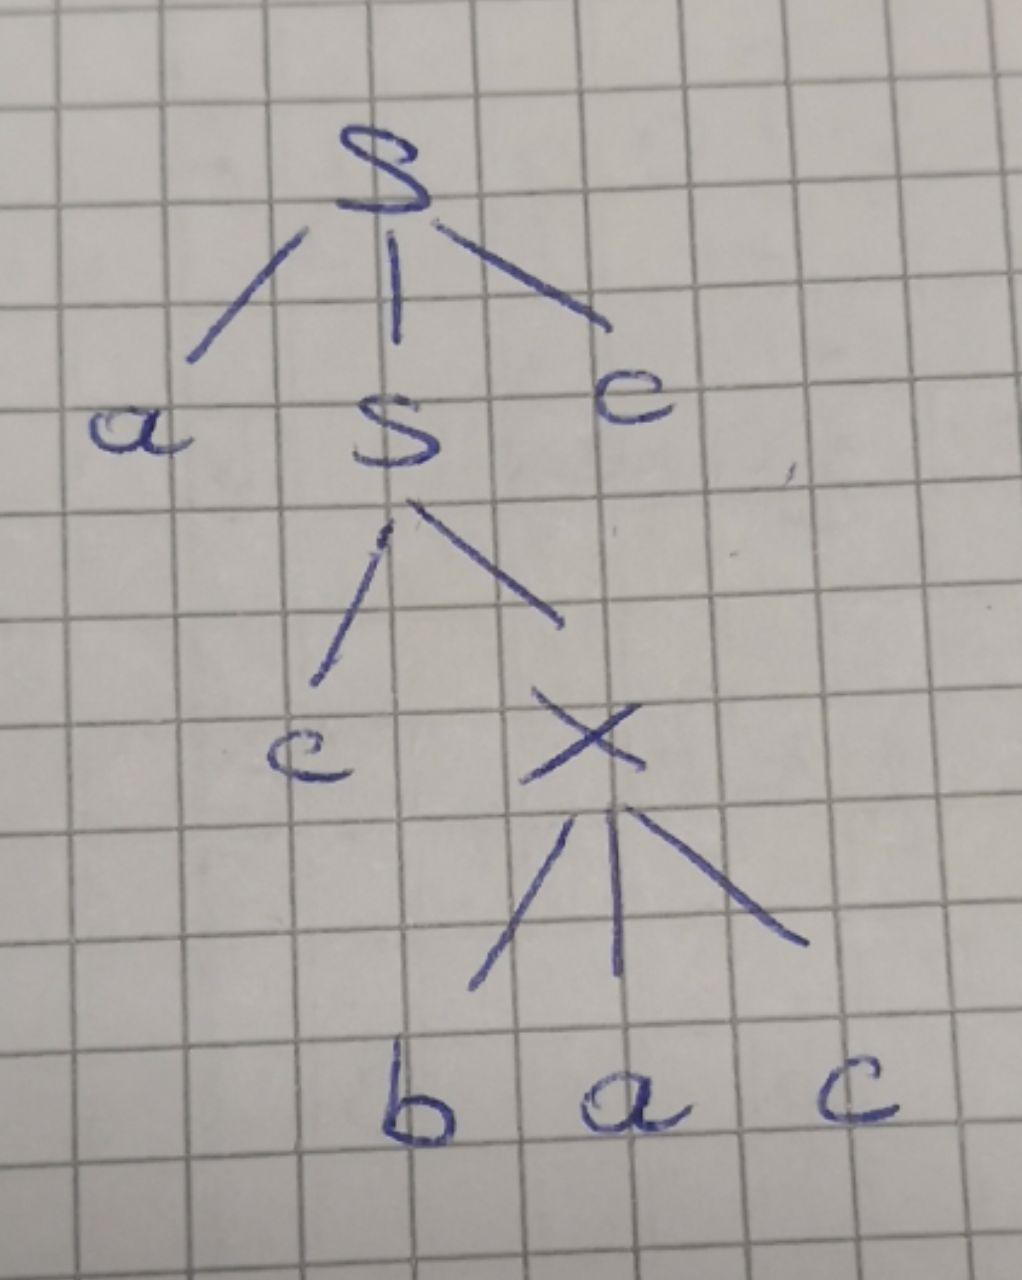
\includegraphics[width=0.75\textwidth]{deriva1}
\end{center}
\section{Esercizio 3}
Progettare un DFA per L = \{$w \in \{a, b, c, d\}^{\star}$ | w inizia con a oppure
c, e termina con d, ed è contenente un numero pari di b\} 
\paragraph{Esempio: } 
\begin{itemize}
	\item abcbd, cd, cbbdbabad $\in$ L \\
	\item bbd, cbdbbd $\notin$ L
\end{itemize}
\begin{center}
\begin{tikzpicture}[scale=0.2]
\tikzstyle{every node}+=[inner sep=0pt]
\draw [black] (13.6,-21.2) circle (3);
\draw (13.6,-21.2) node {$q_0$};
\draw [black] (34.7,-21.2) circle (3);
\draw (34.7,-21.2) node {$q_1$};
\draw [black] (55.5,-22.2) circle (3);
\draw (55.5,-22.2) node {$q_2$};
\draw [black] (55.5,-22.2) circle (2.4);
\draw [black] (16.3,-37.5) circle (3);
\draw (16.3,-37.5) node {$qe$};
\draw [black] (35.6,-37.8) circle (3);
\draw (35.6,-37.8) node {$q_3$};
\draw [black] (7.9,-21.2) -- (10.6,-21.2);
\draw (7.4,-21.2) node [left] {$start$};
\fill [black] (10.6,-21.2) -- (9.8,-20.7) -- (9.8,-21.7);
\draw [black] (16.6,-21.2) -- (31.7,-21.2);
\fill [black] (31.7,-21.2) -- (30.9,-20.7) -- (30.9,-21.7);
\draw (24.15,-21.7) node [below] {$a,c$};
\draw [black] (33.377,-18.52) arc (234:-54:2.25);
\draw (34.7,-13.95) node [above] {$a,c$};
\fill [black] (36.02,-18.52) -- (36.9,-18.17) -- (36.09,-17.58);
\draw [black] (37.346,-19.793) arc (113.19962:61.29541:17.908);
\fill [black] (53,-20.55) -- (52.54,-19.72) -- (52.06,-20.6);
\draw (45.31,-17.82) node [above] {$d$};
\draw [black] (58.406,-21.504) arc (131.19573:-156.80427:2.25);
\draw (62.83,-24.09) node [right] {$d$};
\fill [black] (57.82,-24.08) -- (57.97,-25.01) -- (58.72,-24.36);
\draw [black] (14.09,-24.16) -- (15.81,-34.54);
\fill [black] (15.81,-34.54) -- (16.17,-33.67) -- (15.19,-33.83);
\draw (14.24,-29.57) node [left] {$b,\mbox{ }d$};
\draw [black] (33.925,-35.318) arc (-152.22764:-201.56564:13.761);
\fill [black] (33.92,-35.32) -- (33.99,-34.38) -- (33.11,-34.84);
\draw (31.78,-29.68) node [left] {$b$};
\draw [black] (36.015,-23.893) arc (21.21787:-15.01115:17.858);
\fill [black] (36.01,-23.89) -- (35.84,-24.82) -- (36.77,-24.46);
\draw (37.78,-29.36) node [right] {$b$};
\draw [black] (52.581,-22.889) arc (-79.35459:-106.15038:32.497);
\fill [black] (37.54,-22.17) -- (38.17,-22.87) -- (38.45,-21.91);
\draw (44.93,-24) node [below] {$a,\mbox{ }c$};
\draw [black] (53.14,-24.05) -- (37.96,-35.95);
\fill [black] (37.96,-35.95) -- (38.9,-35.85) -- (38.28,-35.06);
\draw (44.54,-29.5) node [above] {$b$};
\draw [black] (34.984,-40.724) arc (15.84277:-272.15723:2.25);
\draw (28.54,-43.6) node [below] {$a,\mbox{ }c,\mbox{ }d$};
\fill [black] (32.9,-39.09) -- (32,-38.83) -- (32.27,-39.79);
\draw [black] (16.479,-40.483) arc (31.16635:-256.83365:2.25);
\draw (10.16,-44.27) node [below] {$a,\mbox{ }b,\mbox{ }c\mbox{ }d$};
\fill [black] (14.04,-39.46) -- (13.1,-39.44) -- (13.62,-40.3);
\end{tikzpicture}
\end{center}
\section{Esercizio 4}
Data la seguente ER =$aa^{\star}(bb+c)^{\star}(b+a)$
\begin{itemize}
	\item La stringa abbca appartiene? Sì
	\item La stringa bbcb? No
	\item aab? Sì
	\paragraph{Precisazione: }Bisogna dare un occhio alla stringa basandosi sulla 
	ER che ci vien fornita, quindi non è così istantanea la risposta
	\item abbba? 
\end{itemize}
\section{Esercizio 5}
Trasformazione di un $\epsilon$-NFA $\to$ DFA
\begin{center}
\begin{tikzpicture}[scale=0.2]
\tikzstyle{every node}+=[inner sep=0pt]
\draw [black] (26.9,-12.5) circle (3);
\draw (26.9,-12.5) node {$q_0$};
\draw [black] (45.2,-11.4) circle (3);
\draw (45.2,-11.4) node {$q_1$};
\draw [black] (60,-12.7) circle (3);
\draw (60,-12.7) node {$q_2$};
\draw [black] (48.6,-28.1) circle (3);
\draw (48.6,-28.1) node {$q_3$};
\draw [black] (36.2,-28.6) circle (3);
\draw (36.2,-28.6) node {$q_4$};
\draw [black] (12.4,-14.5) -- (23.93,-12.91);
\draw (11.72,-14.66) node [left] {$start$};
\fill [black] (23.93,-12.91) -- (23.07,-12.52) -- (23.2,-13.51);
\draw [black] (29.89,-12.32) -- (42.21,-11.58);
\fill [black] (42.21,-11.58) -- (41.38,-11.13) -- (41.44,-12.13);
\draw (36.12,-12.51) node [below] {$b$};
\draw [black] (48.19,-11.66) -- (57.01,-12.44);
\fill [black] (57.01,-12.44) -- (56.26,-11.87) -- (56.17,-12.87);
\draw (52.46,-12.62) node [below] {$\epsilon$};
\draw [black] (62.68,-11.377) arc (144:-144:2.25);
\draw (67.25,-12.7) node [right] {$a$};
\fill [black] (62.68,-14.02) -- (63.03,-14.9) -- (63.62,-14.09);
\draw [black] (45.8,-14.34) -- (48,-25.16);
\fill [black] (48,-25.16) -- (48.33,-24.28) -- (47.35,-24.48);
\draw (46.16,-20.07) node [left] {$a$};
\draw [black] (58.22,-15.11) -- (50.38,-25.69);
\fill [black] (50.38,-25.69) -- (51.26,-25.34) -- (50.46,-24.75);
\draw (53.72,-19.01) node [left] {$\epsilon$};
\draw [black] (45.6,-28.22) -- (39.2,-28.48);
\fill [black] (39.2,-28.48) -- (40.02,-28.95) -- (39.98,-27.95);
\draw (42.37,-27.81) node [above] {$b$};
\draw [black] (34.7,-26) -- (28.4,-15.1);
\fill [black] (28.4,-15.1) -- (28.37,-16.04) -- (29.23,-15.54);
\draw (32.2,-19.32) node [right] {$\epsilon$};
\end{tikzpicture}
\end{center}
A questo punto bisogna calcolarsi gli ECLOSE
\begin{itemize}
	\item ECLOSE($q_{0}$) = \{$q_{0}$\}
	\item ECLOSE($q_{1}$) = \{$q_{1}$, $q_{2}$, $q_{3}$\}
	\item ECLOSE($q_{2}$) = \{$q_{2}$, $q_{3}$\}
	\item ECLOSE($q_{3}$) = \{$q_{3}$\}
	\item ECLOSE($q_{4}$) = \{$q_{0}$, $q_{4}$\}
\end{itemize}
\begin{center}
\begin{tabular}{ |c|c|c| } 
\hline
~ & a & b \\ 
\hline
$\to {q_{0}}$ & $\varnothing$ & ${q_{1}, q_{2}, q_{3}}$ \\ 
$\varnothing$ & $\varnothing$ & $\varnothing$ \\
$\star {q_{1}, q_{2}, q_{3}}$ & ${q_{2}, q_{3}}$ & ${q_{0}, q_{4}}$\\  
$\star {q_{2}, q_{3}}$ & \{${q_{2}, q_{3}}$\} & \{$q_{0}, q_{4}$\} \\
$\star {q_{0}, q_{4}}$ & $\varnothing$ & \{$q_{1}, q_{2}, q_{3}$\} \\
\hline
\end{tabular}
\end{center}  

\begin{center}
\begin{tabular}{ |c|c|c| } 
\hline
~ & a & b \\ 
\hline
A & B & C \\ 
B & B & B \\ 
C & D & E \\ 
D & D & E \\ 
E & B & C \\ 
\hline
\end{tabular}
\end{center} 
\begin{center}
\begin{tikzpicture}[scale=0.2]
\tikzstyle{every node}+=[inner sep=0pt]
\draw [black] (20.1,-13.5) circle (3);
\draw (20.1,-13.5) node {$A$};
\draw [black] (43,-13.4) circle (3);
\draw (43,-13.4) node {$C$};
\draw [black] (43,-13.4) circle (2.4);
\draw [black] (65.1,-14.5) circle (3);
\draw (65.1,-14.5) node {$E$};
\draw [black] (50,-30.5) circle (3);
\draw (50,-30.5) node {$D$};
\draw [black] (50,-30.5) circle (2.4);
\draw [black] (30,-29.5) circle (3);
\draw (30,-29.5) node {$B$};
\draw [black] (13.4,-8) -- (17.78,-11.6);
\draw (12.84,-6.57) node [left] {$start$};
\fill [black] (17.78,-11.6) -- (17.48,-10.7) -- (16.85,-11.48);
\draw [black] (23.1,-13.49) -- (40,-13.41);
\fill [black] (40,-13.41) -- (39.2,-12.92) -- (39.2,-13.92);
\draw (31.55,-13.95) node [below] {$b$};
\draw [black] (45.67,-12.038) arc (112.65476:61.64629:19.659);
\fill [black] (62.58,-12.88) -- (62.11,-12.06) -- (61.64,-12.94);
\draw (54.27,-10) node [above] {$b$};
\draw [black] (62.289,-15.543) arc (-73.14077:-112.55817:24.635);
\fill [black] (45.69,-14.72) -- (46.24,-15.49) -- (46.62,-14.56);
\draw (53.87,-17.12) node [below] {$b$};
\draw [black] (62.34,-15.68) -- (32.76,-28.32);
\fill [black] (32.76,-28.32) -- (33.69,-28.47) -- (33.3,-27.55);
\draw (46.63,-21.49) node [above] {$a$};
\draw [black] (63.04,-16.68) -- (52.06,-28.32);
\fill [black] (52.06,-28.32) -- (52.97,-28.08) -- (52.24,-27.39);
\draw (57.02,-21.03) node [left] {$b$};
\draw [black] (47.152,-29.586) arc (-115.66482:-199.81104:10.915);
\fill [black] (47.15,-29.59) -- (46.65,-28.79) -- (46.21,-29.69);
\draw (41.04,-24.79) node [left] {$a$};
\draw [black] (21.68,-16.05) -- (28.42,-26.95);
\fill [black] (28.42,-26.95) -- (28.43,-26.01) -- (27.58,-26.53);
\draw (24.42,-22.79) node [left] {$a$};
\draw [black] (30.327,-32.47) arc (34.01689:-253.98311:2.25);
\draw (25.89,-36.4) node [below] {$a,\mbox{ }b$};
\fill [black] (27.84,-31.57) -- (26.9,-31.6) -- (27.46,-32.43);
\draw [black] (52.381,-32.305) arc (80.56505:-207.43495:2.25);
\draw (54.01,-37.04) node [below] {$d$};
\fill [black] (50.02,-33.49) -- (49.39,-34.2) -- (50.38,-34.36);
\end{tikzpicture}
\end{center}
\paragraph{Questo è lo schema dei passaggi fattibili nei vari schemi}
\begin{center}
\begin{tikzpicture}[scale=0.2]
\tikzstyle{every node}+=[inner sep=0pt]
\draw [black] (18.6,-12.6) circle (3);
\draw (18.6,-12.6) node {$DFA$};
\draw [black] (48.4,-12.6) circle (3);
\draw (48.4,-12.6) node {$NFA$};
\draw [black] (18.6,-30.9) circle (3);
\draw (18.6,-30.9) node {$ER$};
\draw [black] (48.4,-30.9) circle (3);
\draw (48.4,-30.9) node {$\epsilon-NFA$};
\draw [black] (21.143,-11.012) arc (118.64976:61.35024:25.773);
\fill [black] (45.86,-11.01) -- (45.39,-10.19) -- (44.92,-11.07);
\draw [black] (48.4,-15.6) -- (48.4,-27.9);
\fill [black] (48.4,-27.9) -- (48.9,-27.1) -- (47.9,-27.1);
\draw [black] (21.524,-13.268) arc (75.42073:41.4716:50.159);
\fill [black] (46.48,-28.59) -- (46.33,-27.66) -- (45.58,-28.33);
\draw [black] (45.528,-30.034) arc (-108.14405:-134.96361:62.888);
\fill [black] (20.67,-14.77) -- (20.88,-15.69) -- (21.59,-14.98);
\draw [black] (21.6,-30.9) -- (45.4,-30.9);
\fill [black] (45.4,-30.9) -- (44.6,-30.4) -- (44.6,-31.4);
\draw [black] (18.6,-15.6) -- (18.6,-27.9);
\fill [black] (18.6,-27.9) -- (19.1,-27.1) -- (18.1,-27.1);
\end{tikzpicture}
\end{center}
\section{Passaggio da ER a $\epsilon$ -NFA}
\begin{enumerate}
	\item Esattamente uno stato finale
	\item Nessun arco entrante nello stato iniziale
	\item Nessun arco uscente dallo stato finale
\end{enumerate}
\begin{itemize}
	\item 
	\begin{enumerate}
		\item \textbf{BASE: } Se R = $\epsilon$ (L(R) = \{$\epsilon$\}), allora
		\begin{center}
		\begin{tikzpicture}[scale=0.2]
		\tikzstyle{every node}+=[inner sep=0pt]
		\draw [black] (18.9,-11.8) circle (3);
		\draw [black] (47.7,-11.9) circle (3);
		\draw [black] (47.7,-11.9) circle (2.4);
		\draw [black] (21.9,-11.81) -- (44.7,-11.89);
		\fill [black] (44.7,-11.89) -- (43.9,-11.39) -- (43.9,-12.39);
		\draw (33.3,-12.35) node [below] {$\epsilon$};
		\end{tikzpicture}
		\end{center}
		\item se R = $\varnothing$ (L(R) = $\varnothing$), allora
		\begin{center}
		\begin{tikzpicture}[scale=0.2]
		\tikzstyle{every node}+=[inner sep=0pt]
		\draw [black] (18.9,-11.8) circle (3);
		\draw [black] (47.7,-11.9) circle (3);
		\draw [black] (47.7,-11.9) circle (2.4);
		\end{tikzpicture}
		\end{center}
		\item Se R = a (L(R) = \{a\}), allora 
		\begin{center}
		\begin{tikzpicture}[scale=0.2]
		\tikzstyle{every node}+=[inner sep=0pt]
		\draw [black] (18.9,-11.8) circle (3);
		\draw [black] (47.7,-11.9) circle (3);
		\draw [black] (47.7,-11.9) circle (2.4);
		\draw [black] (21.9,-11.81) -- (44.7,-11.89);
		\fill [black] (44.7,-11.89) -- (43.9,-11.39) -- (43.9,-12.39);
		\draw (33.3,-12.35) node [below] {$a$};
		\end{tikzpicture}
		\end{center}
	\end{enumerate}
	\item \textbf{PASSO INDUTTIVO: }
	\begin{enumerate}
		\item Se R = S + T (L(R) = L(S)$\cup$ L(T)), allora
		\begin{center}
		\begin{tikzpicture}[scale=0.2]
		\tikzstyle{every node}+=[inner sep=0pt]
		\draw [black] (12.9,-28.2) circle (3);
		\draw [black] (30.8,-15.7) circle (3);
		\draw [black] (50.1,-15.1) circle (3);
		\draw [black] (64.7,-28.2) circle (3);
		\draw [black] (64.7,-28.2) circle (2.4);
		\draw [black] (52.7,-37.9) circle (3);
		\draw [black] (29.1,-38.5) circle (3);
		\draw [black] (15.36,-26.48) -- (28.34,-17.42);
		\fill [black] (28.34,-17.42) -- (27.4,-17.47) -- (27.97,-18.29);
		\draw (22.8,-22.45) node [below] {$\epsilon$};
		\draw [black] (15.43,-29.81) -- (26.57,-36.89);
		\fill [black] (26.57,-36.89) -- (26.16,-36.04) -- (25.63,-36.88);
		\draw (20.06,-33.85) node [below] {$\epsilon$};
		\draw [black] (52.33,-17.1) -- (62.47,-26.2);
		\fill [black] (62.47,-26.2) -- (62.21,-25.29) -- (61.54,-26.03);
		\draw (56.44,-22.14) node [below] {$\epsilon$};
		\draw [black] (55.03,-36.01) -- (62.37,-30.09);
		\fill [black] (62.37,-30.09) -- (61.43,-30.2) -- (62.06,-30.98);
		\draw (59.65,-33.54) node [below] {$\epsilon$};
		\end{tikzpicture}
		\end{center}
		\item Se R = ST (L(R) = L(S)L(T)), allora		
		\begin{center}
		\begin{tikzpicture}[scale=0.2]
		\tikzstyle{every node}+=[inner sep=0pt]
		\draw [black] (14.4,-28.6) circle (3);
		\draw [black] (32.6,-28.8) circle (3);
		\draw [black] (49.1,-28.2) circle (3);
		\draw [black] (65.3,-27.4) circle (3);
		\draw [black] (65.3,-27.4) circle (2.4);
		\draw [black] (35.6,-28.69) -- (46.1,-28.31);
		\fill [black] (46.1,-28.31) -- (45.28,-27.84) -- (45.32,-28.84);
		\draw (40.88,-29.03) node [below] {$\epsilon$};
		\end{tikzpicture}
		\end{center}
		\item Se R = $S^{\star}$ (L(R)= ($L(S))^{\star}$), allora
		\begin{center}
		\begin{tikzpicture}[scale=0.2]
		\tikzstyle{every node}+=[inner sep=0pt]
		\draw [black] (12.5,-23.6) circle (3);
		\draw [black] (29.1,-23.7) circle (3);
		\draw [black] (46.6,-24) circle (3);
		\draw [black] (60.5,-25.5) circle (3);
		\draw [black] (60.5,-25.5) circle (2.4);
		\draw [black] (15.5,-23.62) -- (26.1,-23.68);
		\fill [black] (26.1,-23.68) -- (25.3,-23.18) -- (25.3,-24.18);
		\draw (20.8,-24.16) node [below] {$\epsilon$};
		\draw [black] (58.05,-27.229) arc (-57.07682:-127.45673:37.548);
		\fill [black] (58.05,-27.23) -- (57.11,-27.24) -- (57.65,-28.08);
		\draw (36.13,-33.77) node [below] {$\epsilon$};
		\draw [black] (28.806,-20.728) arc (-183.78208:-358.18215:9.107);
		\fill [black] (28.81,-20.73) -- (29.36,-19.96) -- (28.36,-19.9);
		\draw (38.06,-11.71) node [above] {$\epsilon$};
		\draw [black] (49.58,-24.32) -- (57.52,-25.18);
		\fill [black] (57.52,-25.18) -- (56.78,-24.6) -- (56.67,-25.59);
		\draw (53.35,-25.33) node [below] {$\epsilon$};
		\end{tikzpicture}
		\end{center}
		\item Se R = (S) (L(R)=L(S)), allora 
		$\epsilon$-NFA per R = $\epsilon$-NFA per S
	\end{enumerate}
\end{itemize}
\paragraph{Altra trasformazione di un $\epsilon$-NFA $\to$ DFA}
\begin{center}
\begin{tikzpicture}[scale=0.2]
\tikzstyle{every node}+=[inner sep=0pt]
\draw [black] (18.6,-26.6) circle (3);
\draw (18.6,-26.6) node {$q_0$};
\draw [black] (41.1,-15.5) circle (3);
\draw (41.1,-15.5) node {$q_1$};
\draw [black] (41.1,-15.5) circle (2.4);
\draw [black] (62.7,-26.6) circle (3);
\draw (62.7,-26.6) node {$q_2$};
\draw [black] (41.1,-39.4) circle (3);
\draw (41.1,-39.4) node {$q_3$};
\draw [black] (5.9,-23) -- (15.71,-25.78);
\draw (5.13,-22.44) node [left] {$start$};
\fill [black] (15.71,-25.78) -- (15.08,-25.08) -- (14.81,-26.04);
\draw [black] (38.255,-38.449) arc (-109.92665:-129.34348:59.3);
\fill [black] (38.25,-38.45) -- (37.67,-37.71) -- (37.33,-38.65);
\draw (28.2,-34.74) node [below] {$a$};
\draw [black] (43.68,-37.87) -- (60.12,-28.13);
\fill [black] (60.12,-28.13) -- (59.18,-28.11) -- (59.69,-28.97);
\draw (52.9,-33.5) node [below] {$b$};
\draw [black] (59.813,-25.787) arc (-107.31838:-127.07788:53.637);
\fill [black] (43.44,-17.37) -- (43.78,-18.26) -- (44.38,-17.46);
\draw (50.33,-22.79) node [below] {$a$};
\draw [black] (44.042,-16.082) arc (76.60338:49.00036:38.815);
\fill [black] (60.51,-24.55) -- (60.24,-23.64) -- (59.58,-24.4);
\draw (53.73,-18.81) node [above] {$\epsilon$};
\draw [black] (21.29,-25.27) -- (38.41,-16.83);
\fill [black] (38.41,-16.83) -- (37.47,-16.73) -- (37.91,-17.63);
\draw (30.78,-21.55) node [below] {$\epsilon$};
\end{tikzpicture}
\end{center}
\begin{itemize}
	\item ECLOSE($q_{0}$) = \{$q_{0}, q_{1}, q_{2}$\}
	\item ECLOSE($q_{1}$) = \{$q_{1}, q_{2}$\}
	\item ECLOSE($q_{2}$) = \{$q_{2}$\}
	\item ECLOSE($q_{3}$) = \{$q_{2}$\}
\end{itemize}
\begin{center}
\begin{tabular}{ |c|c|c| } 
\hline
~ & a & b \\
\hline 
$\star \to$ \{$q_{0}, q_{1}, q_{2}$\} & \{$q_{1}, q_{2}$\} & \{$q_{3}$\} \\ 
$\star$ \{$q_{1}, q_{2}$\} & \{$q_{1}, q_{2}$\} & \{$q_{3}$\} \\ 
\{$q_{3}$\} & \{$q_{0}, q_{1}, q_{2}$\} & {$q_{2}$} \\ 
\{$q_{2}$\} & \{$q_{1}, q_{2}$\} & $\varnothing$ \\
$\varnothing$ & $\varnothing$ & $\varnothing$ \\
\hline
\end{tabular}
\end{center}
\subparagraph{Sorry: }Non ho fatto la tabella con le lettere prima di fare 
diretto l'automa nuovo, però son facilmente ricavabili.	
\begin{center}
\begin{tikzpicture}[scale=0.2]
\tikzstyle{every node}+=[inner sep=0pt]
\draw [black] (15.7,-14.7) circle (3);
\draw (15.7,-14.7) node {$A$};
\draw [black] (15.7,-14.7) circle (2.4);
\draw [black] (45,-14.7) circle (3);
\draw (45,-14.7) node {$B$};
\draw [black] (45,-14.7) circle (2.4);
\draw [black] (16.3,-37) circle (3);
\draw (16.3,-37) node {$C$};
\draw [black] (45,-37) circle (3);
\draw (45,-37) node {$D$};
\draw [black] (65,-38) circle (3);
\draw (65,-38) node {$E$};
\draw [black] (4.3,-14.7) -- (12.7,-14.7);
\draw (3.8,-14.7) node [left] {$start$};
\fill [black] (12.7,-14.7) -- (11.9,-14.2) -- (11.9,-15.2);
\draw [black] (18.7,-14.7) -- (42,-14.7);
\fill [black] (42,-14.7) -- (41.2,-14.2) -- (41.2,-15.2);
\draw (30.35,-15.2) node [below] {$a$};
\draw [black] (46.687,-12.234) arc (173.35775:-114.64225:2.25);
\draw (51.55,-10.18) node [right] {$a$};
\fill [black] (47.98,-14.54) -- (48.72,-15.13) -- (48.84,-14.13);
\draw [black] (45,-34) -- (45,-17.7);
\fill [black] (45,-17.7) -- (44.5,-18.5) -- (45.5,-18.5);
\draw (45.5,-25.85) node [right] {$a$};
\draw [black] (42.63,-16.54) -- (18.67,-35.16);
\fill [black] (18.67,-35.16) -- (19.61,-35.06) -- (18.99,-34.27);
\draw (29.64,-25.35) node [above] {$b$};
\draw [black] (14.392,-34.691) arc (-145.72015:-211.19742:16.261);
\fill [black] (14.39,-34.69) -- (14.35,-33.75) -- (13.53,-34.31);
\draw (11.03,-25.98) node [left] {$b$};
\draw [black] (16.22,-34) -- (15.78,-17.7);
\fill [black] (15.78,-17.7) -- (15.3,-18.51) -- (16.3,-18.49);
\draw (16.54,-25.84) node [right] {$a$};
\draw [black] (19.3,-37) -- (42,-37);
\fill [black] (42,-37) -- (41.2,-36.5) -- (41.2,-37.5);
\draw (30.65,-37.5) node [below] {$b$};
\draw [black] (48,-37.15) -- (62,-37.85);
\fill [black] (62,-37.85) -- (61.23,-37.31) -- (61.18,-38.31);
\draw (54.95,-38.05) node [below] {$b$};
\draw [black] (67.045,-35.821) arc (164.55605:-123.44395:2.25);
\draw (72.08,-34.81) node [right] {$a,b$};
\fill [black] (67.97,-38.3) -- (68.61,-38.99) -- (68.88,-38.03);
\end{tikzpicture}
\end{center}
\section{$\widehat{\delta}$ per $\epsilon$-NFA}
\paragraph{$\widehat{\delta} Q \times \Sigma^{\star} \to 2^{Q}$}: 
$\widehat{\delta}(q,w) = \{p_{1}, ..., p_{\kappa}\}$
\subsection{$1^{a}$ definizione:}
(w = ax)
\begin{itemize}
	\item \textbf{BASE: } $\widehat{\delta}$(q,$\epsilon$) = ECLOSE(q)
	\item \textbf{PASSO: } $\widehat{\delta}(q, ax) = $\\
	Posto ECLOSE(q) = \{$p_{0}, ..., p_{\kappa}$\} e \{$r_{1}, ..., r_{m}$\} = 
	$\bigcup \limits_{i = 1}^{\kappa} \delta (p_{i}, a)$
\end{itemize}

ECLOSE(S) = $\bigcup \limits_{q \in S}$ ECLOSE(q)\\ 
$\delta$(S,a) = $\bigcup \limits_{q \in S} ~ \delta$(q, a)\\
$\widehat{\delta}(S, w)$ = $\bigcup \limits_{q \in S} \widehat{\delta}$(q, w)\\

\paragraph{}ECLOSE($\varnothing$) = $\varnothing$\\
$\delta$($\varnothing$, a) = $\varnothing ~ \forall a$\\
$\widehat{\delta}(\varnothing, w)$ = $\varnothing ~ \forall w$

\begin{itemize}
	\item \textbf{BASE: }$\widehat{\delta}(q,\epsilon) =$ ECLOSE(q)
	\item \textbf{PASSO: }$\widehat{\delta}(q, ax) = \widehat{\delta}(R, x)$\\
	posto P = ECLOSE(q)\\
	S = $\delta(P,a)$\\
	R = ECLOSE(S)\\
	$\widehat{\delta}(q, ax) = \widehat{\delta}($ECLOSE($\delta$ECLOSE(q),a),x) 
\end{itemize}
\paragraph{Ulteriore estensione: }
$\widehat{\delta} : Q \times \Sigma^{\star} \to 2^{Q} \to \widehat{\delta} 
: 2^{Q} \times \Sigma^{\star} \to 2^{Q}, \widehat{\delta}(T, w)...$

\begin{itemize}
	\item \textbf{BASE: }$\widehat{\delta}(T, \epsilon) = $ ECLOSE(T)
	\item \textbf{PASSO: }$\widehat{\delta}(T, ax) = \widehat{\delta}(R, x)$\\
	posto P = ECLOSE(T)\\
	S = $\delta$(P, a) ed R = ECLOSE(S)
\end{itemize}
\paragraph{Esempio: }
\begin{center}
\begin{tikzpicture}[scale=0.2]
\tikzstyle{every node}+=[inner sep=0pt]
\draw [black] (20.9,-20.1) circle (3);
\draw (20.9,-20.1) node {$q_0$};
\draw [black] (42.4,-20.1) circle (3);
\draw (42.4,-20.1) node {$q_1$};
\draw [black] (63.3,-20.1) circle (3);
\draw (63.3,-20.1) node {$q_2$};
\draw [black] (63.3,-20.1) circle (2.4);
\draw [black] (19.942,-17.269) arc (226.43416:-61.56584:2.25);
\draw (22.08,-12.82) node [above] {$a$};
\fill [black] (22.56,-17.62) -- (23.48,-17.38) -- (22.75,-16.69);
\draw [black] (40.694,-17.646) arc (242.53789:-45.46211:2.25);
\draw (41.02,-12.83) node [above] {$b$};
\fill [black] (43.31,-17.25) -- (44.12,-16.77) -- (43.24,-16.31);
\draw [black] (7.2,-22.4) -- (17.94,-20.6);
\draw (6.49,-22.63) node [left] {$start$};
\fill [black] (17.94,-20.6) -- (17.07,-20.24) -- (17.24,-21.22);
\draw [black] (23.9,-20.1) -- (39.4,-20.1);
\fill [black] (39.4,-20.1) -- (38.6,-19.6) -- (38.6,-20.6);
\draw (31.65,-20.6) node [below] {$\epsilon$};
\draw [black] (45.4,-20.1) -- (60.3,-20.1);
\fill [black] (60.3,-20.1) -- (59.5,-19.6) -- (59.5,-20.6);
\draw (52.85,-20.6) node [below] {$\epsilon$};
\draw [black] (63.121,-17.117) arc (211.16635:-76.83365:2.25);
\draw (66.83,-13.37) node [above] {$c$};
\fill [black] (65.56,-18.14) -- (66.5,-18.16) -- (65.98,-17.3);
\end{tikzpicture}
\end{center}
\paragraph{Considerando la stringa w = aabc: }
\subparagraph{*Incompleto, finitelo voi please*}	
$\widehat{\delta}$($q_{0}$, aabc) x=abc
\\ P = ECLOSE($q_{0}$) = \{$q_{0}, q_{1}, q_{2}$\}\\
S = $\delta$(P, a) = \{$q_{0}$\}\\
R = ECLOSE(S) = ECLOSE($q_{0}$) \{$q_{0}, q_{1}, q_{2}$\}\\
$\widehat{\delta}(q_{0}, aabc) = \widehat{\delta}(\underbrace{\{q_{0}, q_{1},
q_{2}\}}_{P}, \underbrace{abc}_{x})$
\section{Trasformazione da automa a ER}
Questo algoritmo funziona per eliminazione degli stati, quindi l'idea è che
io parta da un automa complesso in cui ho uno stato iniziale, alcuni stati finali,
e degli stai che non sono nè iniziali nè finali. \\ 
Come casi particolari ho la situazione in cui lo stato iniziale è anche finale.
In seguito ci sono stati che non sono nè iniziali nè finali, e son quelli che 
andremo ad elidere.
\paragraph{Alla fine }si ottiene un automa semplificato avente uno stato iniziale
ed uno o più finali. 
\begin{center}
\begin{tikzpicture}[scale=0.2]
\tikzstyle{every node}+=[inner sep=0pt]
\draw [black] (20.8,-30.8) circle (3);
\draw [black] (36.2,-19.7) circle (3);
\draw [black] (36.2,-19.7) circle (2.4);
\draw [black] (36.2,-30.8) circle (3);
\draw [black] (36.2,-30.8) circle (2.4);
\draw [black] (36.2,-41.7) circle (3);
\draw [black] (36.2,-41.7) circle (2.4);
\draw [black] (10.3,-30.8) -- (17.8,-30.8);
\fill [black] (17.8,-30.8) -- (17,-30.3) -- (17,-31.3);
\draw [black] (23.23,-29.05) -- (33.77,-21.45);
\fill [black] (33.77,-21.45) -- (32.82,-21.52) -- (33.41,-22.33);
\draw [black] (23.25,-32.53) -- (33.75,-39.97);
\fill [black] (33.75,-39.97) -- (33.39,-39.1) -- (32.81,-39.91);
\draw [black] (23.8,-30.8) -- (33.2,-30.8);
\fill [black] (33.2,-30.8) -- (32.4,-30.3) -- (32.4,-31.3);
\draw [black] (36.2,-27.8) -- (36.2,-22.7);
\fill [black] (36.2,-22.7) -- (35.7,-23.5) -- (36.7,-23.5);
\draw [black] (36.2,-22.7) -- (36.2,-27.8);
\fill [black] (36.2,-27.8) -- (36.7,-27) -- (35.7,-27);
\draw [black] (36.2,-33.8) -- (36.2,-38.7);
\fill [black] (36.2,-38.7) -- (36.7,-37.9) -- (35.7,-37.9);
\draw [black] (36.2,-38.7) -- (36.2,-33.8);
\fill [black] (36.2,-33.8) -- (35.7,-34.6) -- (36.7,-34.6);
\end{tikzpicture}
\end{center}
ER = $ER_{1} + ER_{2} + ER_{3} = 
\begin{cases}
L_{1} \to ER_{1}\\
L_{2} \to ER_{2}\\
L_{3} \to ER_{3}\\
\end{cases}$
\paragraph{Esempio fig 3.7 p 92}
\begin{center}
\begin{tikzpicture}[scale=0.2]
\tikzstyle{every node}+=[inner sep=0pt]
\draw [black] (18.5,-15.6) circle (3);
\draw (18.5,-15.6) node {$q_1$};
\draw [black] (45.6,-29) circle (3);
\draw (45.6,-29) node {$S$};
\draw [black] (22.4,-41.9) circle (3);
\draw (22.4,-41.9) node {$q_\kappa$};
\draw [black] (62.6,-13.1) circle (3);
\draw (62.6,-13.1) node {$p_1$};
\draw [black] (62.6,-40.2) circle (3);
\draw (62.6,-40.2) node {$pm$};
\draw [black] (21.19,-16.93) -- (42.91,-27.67);
\fill [black] (42.91,-27.67) -- (42.42,-26.87) -- (41.97,-27.76);
\draw (33.68,-21.79) node [above] {$Q_1$};
\draw [black] (25.02,-40.44) -- (42.98,-30.46);
\fill [black] (42.98,-30.46) -- (42.04,-30.41) -- (42.52,-31.28);
\draw (36.27,-35.95) node [below] {$Q_\kappa$};
\draw [black] (43.623,-26.759) arc (249.14944:-38.85056:2.25);
\draw (43.02,-21.92) node [above] {$S$};
\fill [black] (46.18,-26.07) -- (46.93,-25.5) -- (45.99,-25.14);
\draw [black] (47.79,-26.95) -- (60.41,-15.15);
\fill [black] (60.41,-15.15) -- (59.48,-15.33) -- (60.17,-16.06);
\draw (55.76,-21.53) node [below] {$Q_1$};
\draw [black] (62.6,-16.1) -- (62.6,-37.2);
\fill [black] (62.6,-37.2) -- (63.1,-36.4) -- (62.1,-36.4);
\draw [black] (48.11,-30.65) -- (60.09,-38.55);
\fill [black] (60.09,-38.55) -- (59.7,-37.69) -- (59.15,-38.53);
\draw (51.76,-35.1) node [below] {$P_m$};
\draw [black] (61.597,-43.025) arc (-22.86995:-215.43763:25.904);
\fill [black] (61.6,-43.03) -- (60.82,-43.57) -- (61.75,-43.96);
\draw (22.67,-56.08) node [below] {$R1m$};
\draw [black] (21.5,-15.43) -- (59.6,-13.27);
\fill [black] (59.6,-13.27) -- (58.78,-12.82) -- (58.83,-13.81);
\draw (40.68,-14.96) node [below] {$R_{11}$};
\draw [black] (25.4,-41.77) -- (59.6,-40.33);
\fill [black] (59.6,-40.33) -- (58.78,-39.86) -- (58.82,-40.86);
\draw (42.39,-40.43) node [above] {$R_{\kappa m}$};
\draw [black] (18.94,-18.57) -- (21.96,-38.93);
\fill [black] (21.96,-38.93) -- (22.34,-38.07) -- (21.35,-38.21);
\draw [black] (64.708,-15.232) arc (41.27166:-150.03468:25.321);
\fill [black] (64.71,-15.23) -- (64.86,-16.16) -- (65.61,-15.5);
\draw (63.15,-53.02) node [below] {$R_{\kappa 1}$};
\end{tikzpicture}
\end{center}
$q_{1}, ..., q_{\kappa}$ sono predecessori di S \\
$p_{1}, ..., p_{m}$ sono successori di S\\
$Q_{1}, ..., Q_{\kappa}, p_{1}, ..., p_{m}, S$ sono ER \\
$R_{1j} \forall i \forall j$ sono ER, Se $\nexists$ arco da $q_{1}$ a $p_{j}$, 
allora $R_{1j}$ = $\varnothing$, stessa cosa invece per S
\begin{center}
\begin{tikzpicture}[scale=0.2]
\tikzstyle{every node}+=[inner sep=0pt]
\draw [black] (19.1,-13.4) circle (3);
\draw (19.1,-13.4) node {$q_1$};
\draw [black] (49.9,-13.4) circle (3);
\draw (49.9,-13.4) node {$p_1$};
\draw [black] (49.9,-34.7) circle (3);
\draw (49.9,-34.7) node {$p_m$};
\draw [black] (19.1,-34.7) circle (3);
\draw (19.1,-34.7) node {$q_\kappa$};
\draw [black] (22.1,-13.4) -- (46.9,-13.4);
\fill [black] (46.9,-13.4) -- (46.1,-12.9) -- (46.1,-13.9);
\draw (34.5,-12.9) node [above] {$R_11\mbox{ }+\mbox{ }Q_1\mbox{ }S^\star\mbox{ }P_1$};
\draw [black] (19.1,-16.4) -- (19.1,-31.7);
\fill [black] (19.1,-31.7) -- (19.6,-30.9) -- (18.6,-30.9);
\draw (18.6,-24.05) node [left] {$R_\kappa1\mbox{ }+\mbox{ }Q_\kappa\mbox{ }S^\star\mbox{ }P_1$};
\draw [black] (49.9,-16.4) -- (49.9,-31.7);
\fill [black] (49.9,-31.7) -- (50.4,-30.9) -- (49.4,-30.9);
\draw [black] (22.1,-34.7) -- (46.9,-34.7);
\fill [black] (46.9,-34.7) -- (46.1,-34.2) -- (46.1,-35.2);
\draw (34.5,-35.2) node [below] {$R_\kappa\mbox{ }m\mbox{ }+\mbox{ }Q_\kappa\mbox{ }S^\star\mbox{ }P_m$};
\draw [black] (21.749,-14.808) arc (61.43212:49.23563:148.204);
\fill [black] (47.65,-32.72) -- (47.37,-31.82) -- (46.72,-32.57);
\draw (45.08,-22.57) node [above] {$R_1\mbox{ }m\mbox{ }+\mbox{ }Q_0\mbox{ }S^\star\mbox{ }P_m$};
\draw [black] (20.515,-32.056) arc (149.58966:99.74259:38.1);
\fill [black] (20.52,-32.06) -- (21.35,-31.62) -- (20.49,-31.11);
\end{tikzpicture}
\end{center}
Se per esempio avessi
\begin{itemize}
	\item Stato iniziale $q_{0}$
	\item Stati finali $q_{1}, ..., q_{m}$
\end{itemize}

\begin{center}
\begin{tikzpicture}[scale=0.2]
\tikzstyle{every node}+=[inner sep=0pt]
\draw [black] (25.5,-24.7) circle (3);
\draw (25.5,-24.7) node {$q_0$};
\draw [black] (49.3,-24.7) circle (3);
\draw (49.3,-24.7) node {$q_1$};
\draw [black] (49.3,-24.7) circle (2.4);
\draw [black] (11.3,-24.7) -- (22.5,-24.7);
\draw (10.8,-24.7) node [left] {$start$};
\fill [black] (22.5,-24.7) -- (21.7,-24.2) -- (21.7,-25.2);
\draw [black] (27.204,-22.239) arc (138.94194:41.05806:13.521);
\fill [black] (47.6,-22.24) -- (47.45,-21.31) -- (46.69,-21.96);
\draw (37.4,-17.1) node [above] {$S$};
\draw [black] (52.06,-25.846) arc (95.18593:-192.81407:2.25);
\draw (54.98,-30.27) node [below] {$U$};
\fill [black] (50.07,-27.59) -- (49.64,-28.43) -- (50.64,-28.34);
\draw [black] (47.416,-27.028) arc (-45.0462:-134.9538:14.177);
\fill [black] (27.38,-27.03) -- (27.6,-27.95) -- (28.3,-27.24);
\draw (37.4,-31.67) node [below] {$T$};
\draw [black] (25.829,-27.67) arc (34.05477:-253.94523:2.25);
\draw (22.12,-31.58) node [below] {$R$};
\fill [black] (23.34,-26.77) -- (22.4,-26.8) -- (22.96,-27.63);
\end{tikzpicture}
\end{center}
$E_{i}$ = $(R+SU^{\star}T)^{\star}SU^{\star}$\\
$q_{0} $ NON E' STATO FINALE

\begin{center}
\begin{tikzpicture}[scale=0.2]
\tikzstyle{every node}+=[inner sep=0pt]
\draw [black] (43,-27.4) circle (3);
\draw (43,-27.4) node {$q_0$};
\draw [black] (43,-27.4) circle (2.4);
\draw [black] (45.286,-29.325) arc (77.62938:-210.37062:2.25);
\draw (46.84,-34.1) node [below] {$R$};
\fill [black] (42.86,-30.39) -- (42.2,-31.06) -- (43.18,-31.27);
\draw [black] (29.6,-25.8) -- (40.02,-27.04);
\draw (28.94,-25.68) node [left] {$start$};
\fill [black] (40.02,-27.04) -- (39.29,-26.45) -- (39.17,-27.45);
\end{tikzpicture}
\end{center}
$E_{i} = R^{\star}$
\begin{center}
\begin{tikzpicture}[scale=0.2]
\tikzstyle{every node}+=[inner sep=0pt]
\draw [black] (17.6,-23.2) circle (3);
\draw (17.6,-23.2) node {$q_0$};
\draw [black] (37.5,-23.2) circle (3);
\draw (37.5,-23.2) node {$q_1$};
\draw [black] (57.6,-23.2) circle (3);
\draw (57.6,-23.2) node {$q_2$};
\draw [black] (57.6,-23.2) circle (2.4);
\draw [black] (10.2,-23.2) -- (14.6,-23.2);
\draw (9.7,-23.2) node [left] {$start$};
\fill [black] (14.6,-23.2) -- (13.8,-22.7) -- (13.8,-23.7);
\draw [black] (20.6,-23.2) -- (34.5,-23.2);
\fill [black] (34.5,-23.2) -- (33.7,-22.7) -- (33.7,-23.7);
\draw (27.55,-23.7) node [below] {$1$};
\draw [black] (39.905,-21.416) arc (120.80831:59.19169:14.926);
\fill [black] (55.19,-21.42) -- (54.76,-20.58) -- (54.25,-21.44);
\draw (47.55,-18.81) node [above] {$0+1$};
\draw [black] (55.043,-24.762) arc (-63.67449:-116.32551:16.896);
\fill [black] (40.06,-24.76) -- (40.55,-25.56) -- (41,-24.67);
\draw (47.55,-27.01) node [below] {$0,\mbox{ }1$};
\draw [black] (16.277,-20.52) arc (234:-54:2.25);
\draw (17.6,-15.95) node [above] {$0$};
\fill [black] (18.92,-20.52) -- (19.8,-20.17) -- (18.99,-19.58);
\end{tikzpicture}
\end{center}
Eliminiamo $q_{1}$:
pred: $q_{0}, q_{2},~~~ ER q_{0} \xrightarrow{1} q_{1}$, $q_{2} \to^{0+1} q_{1}$\\
succ: $q_{2}$, ~~~ ER $q_{1} \xrightarrow{0+1} q_{2}$\\
no Self-Loop, ER $\varnothing$ con $R_{02}$ = $R_{22} = \varnothing$
\begin{center}
\begin{tikzpicture}[scale=0.2]
\tikzstyle{every node}+=[inner sep=0pt]
\draw [black] (23.8,-22.1) circle (3);
\draw (23.8,-22.1) node {$q_0$};
\draw [black] (50.9,-22.1) circle (3);
\draw (50.9,-22.1) node {$q_2$};
\draw [black] (50.9,-22.1) circle (2.4);
\draw [black] (10.1,-20.8) -- (20.81,-21.82);
\draw (9.47,-20.72) node [left] {$start$};
\fill [black] (20.81,-21.82) -- (20.06,-21.24) -- (19.97,-22.24);
\draw [black] (22.477,-19.42) arc (234:-54:2.25);
\draw (23.8,-14.85) node [above] {$0$};
\fill [black] (25.12,-19.42) -- (26,-19.07) -- (25.19,-18.48);
\draw [black] (26.8,-22.1) -- (47.9,-22.1);
\fill [black] (47.9,-22.1) -- (47.1,-21.6) -- (47.1,-22.6);
\draw (37.35,-22.6) node [below] {$1(0+1)$};
\end{tikzpicture}
\end{center}
\begin{itemize}
	\item $R_{02}$ = $\varnothing$ + 1$\varnothing^{\star}(0+1)$ = 1(0+1)
	\item $R_{22}$ = $\varnothing$ + (0+1)$\varnothing^{\star}(0+1)$ = (0+1)(0+1)
\end{itemize}
(Applico $E_{i}$ = $(R+SU^{\star}T)^{\star}SU^{\star}$)
E = (0 + 1(0+1) $((0+1)(0+1))^{\star}\varnothing)^{\star}$ 1(0+1) \\
$((0+1)(0+1))^{\star} = 0^{\star}1(0+1)((0+1)(0+1))^{\star}$. \\
Volendo si può specificare che: 00+01+10+11
\chapter{Altre operazioni sui Linguaggi Regolari}
\section{Unione}
Se L, M $\in$ REG su $\Sigma$ allora L $\cup$ M $\in$ REG
\paragraph{Dimostrazione 1: }
L, M $\in$ REG $\implies \exists$ espressione regolare R, S t.c L = L(S) e M = L(R)
ALLORA L $\cup$ M = L(S+R)
\paragraph{Dimostrazione 2: }
L, M $\in$ REG $\implies \exists$ due ASF R ed S che li accettano. Costruiamo un
$\epsilon - NFA$ che accetti L $\cup$ M
\subparagraph{Siccome} non ho ancora capito una bega di come si fa a fare questo
tipo di grafico, di nuovo, grazie Gaia $\to$
\begin{center}
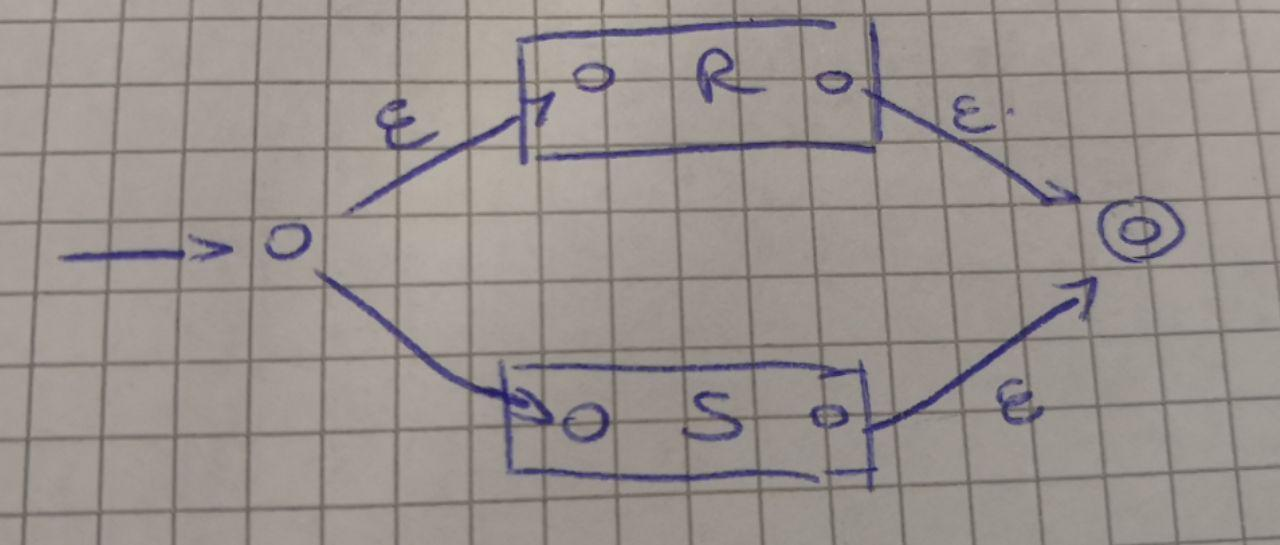
\includegraphics[width=0.75\textwidth]{25}
\end{center}	
\paragraph{Proposizione 1: }Se L, M $\in$ REG, allora LM $\in$ REG 
\paragraph{Proposizione 2: }Se L $\in$ REG, allora $L^{\star} \in$ REG
\paragraph{proposizione 3: }Se L $\in$ REG ($\Sigma$), allora $\overline{L}$
= $\Sigma^{\star}\setminus$L \\
$\in$ REG 
\subparagraph{Dimostrazione: }Se L $\in$ REG $\implies \exists$ DFA, 
A=(Q, $\Sigma, \delta, q_{0}$, F) t.c. L = L(A). Allora $\overline{L} = L(B)$ dove
B è il DFA B = (Q, $\Sigma$, $\delta$, $q_{0}$, Q $\setminus$ F) 	
$\Sigma^{'}$ t.c. $\Sigma \subseteq \Sigma^{'}$\\
L $\subseteq \Sigma^{'~\star}$\\
$\overline{L} = \Sigma^{'~\star} \setminus $L\\
\paragraph{Proposizione 4: }Se L, M $\in$ REG, allora L$\cap$M $\in$ REG
\subparagraph{Dimostrazione: }L$\cap$ M = $\overline{\overline{L} \cup \overline{M}}$	\\
Se L, M $\in$ REG, allora: $\overline{L} \in$ REG, $\overline{M} \in$ REG, 
$\overline{L} \cup \overline{M} \in$ REG, $\overline{\overline{L}\cup\overline{M}} \in$ REG 
\subparagraph{Dimostrazione: }Se L, M $\in$ REG, $\exists$ DFA $A_{L}=(Q_{L}, 
\Sigma, \delta_{L},q_{L}, F_{L}) e A_{M} = (Q_{M}, \Sigma, \delta_{M}, q_{M}, F_{M})$
\begin{center}
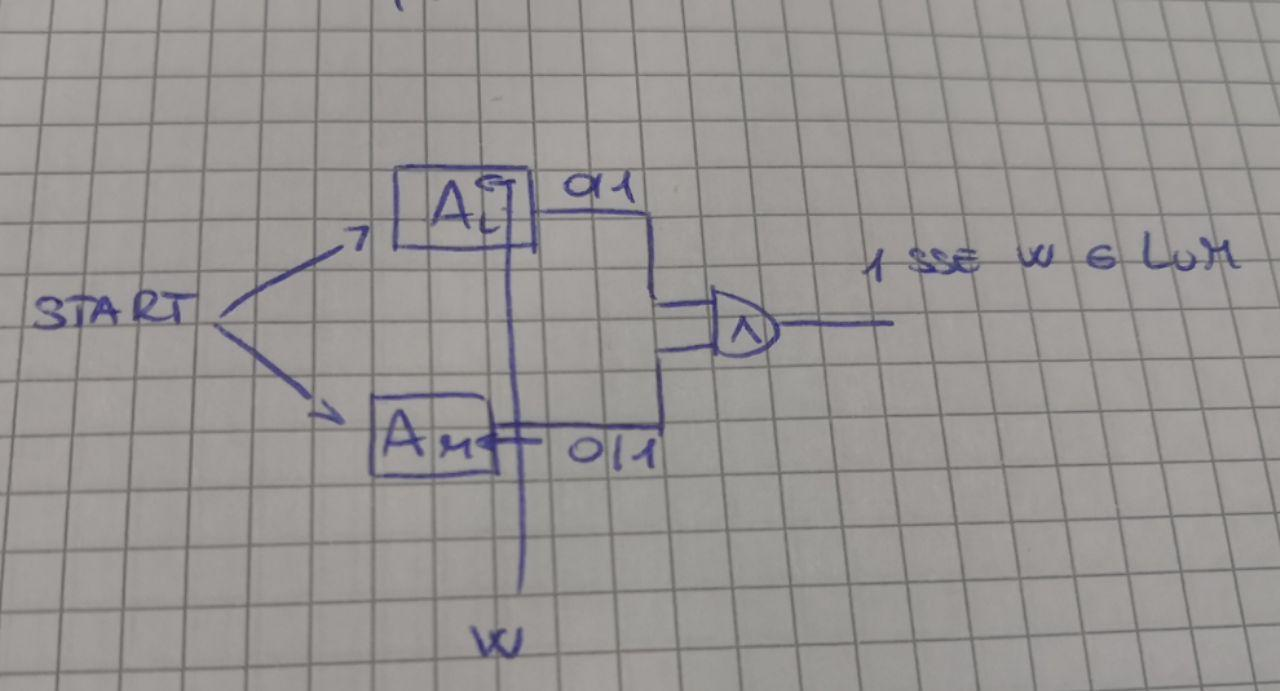
\includegraphics[width=0.75\textwidth]{26}
\end{center}	
\section{Automa Prodotto}
Costruiamo l'automa prodotto $A_{L} \otimes A_{M}$\\
\[A_{L} \oplus A_{M} = (\underbrace{Q_{L} \times Q_{M}}_{Q}, \Sigma, \delta, 
\underbrace{q_{L}, q_{M}}_{q_{0}}, \underbrace{F_{L}\times F_{L}}_{F} \]\\
\[Q = \{(p, q | p \in Q_{L}~ e ~ q\in Q_{M}\}\]
$\delta ((p, q), a) = (\delta_{L}(p,a), \delta_{M}(q,a))$
\section{Differenza insiemistica}
\paragraph{Proposizioni: }Se L, M $\in$ REG, allora L $\setminus$ M $\in$ REG
\subparagraph{Dimostrazione: }L $\setminus$ M = L$\cap \overline{M}$. \\
M $\in$ REG $\implies \overline{M} \in$ REG. L $\cap \overline{M} \in$ REG   
\begin{center}
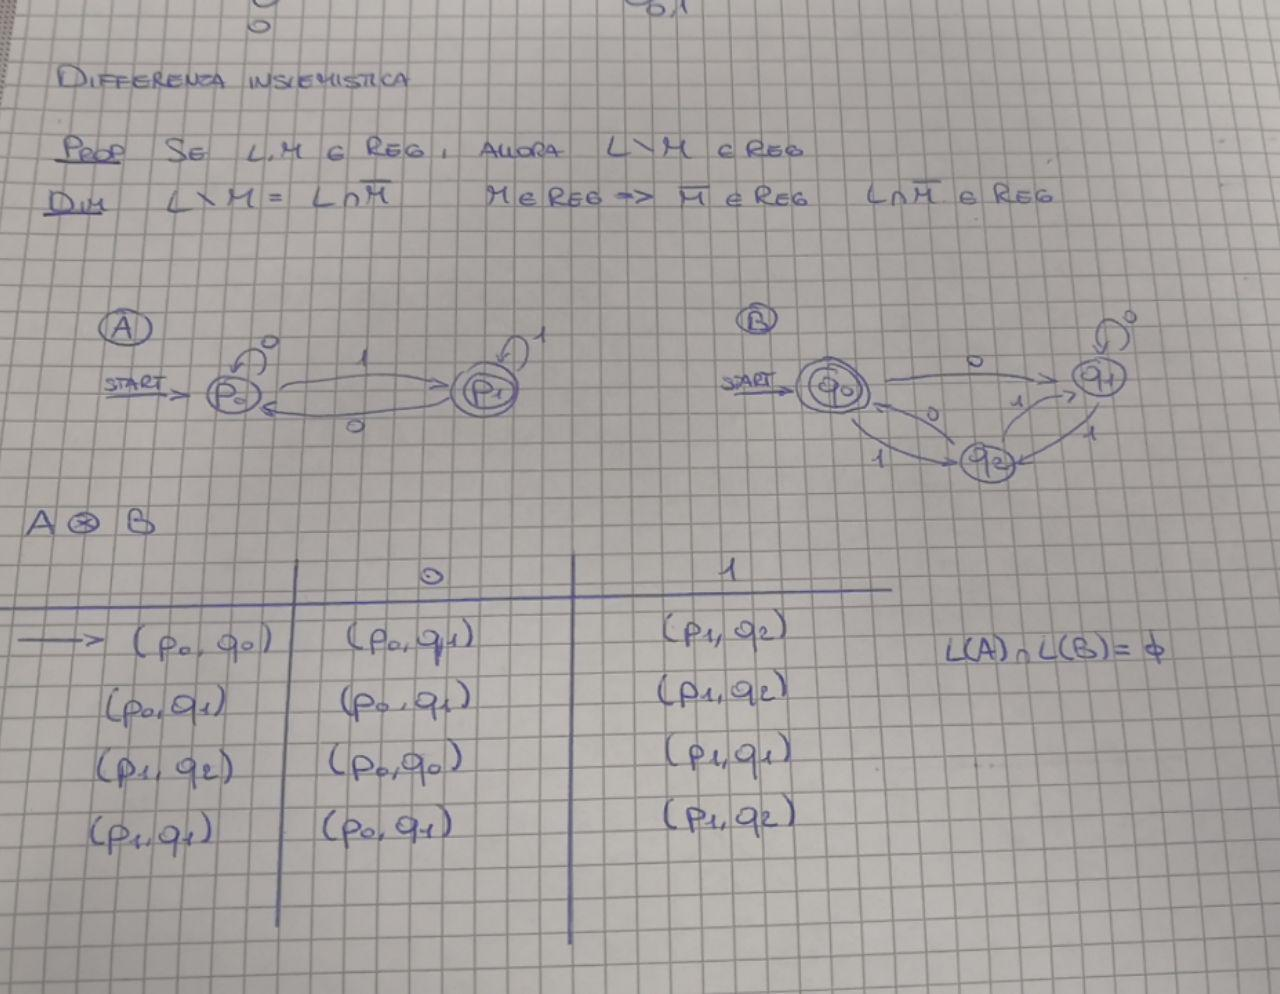
\includegraphics[width=0.75\textwidth]{27}
\end{center}           
















\end{document}